% This is "sig-alternate.tex" V2.0 May 2012
% This file should be compiled with V2.5 of "sig-alternate.cls" May 2012
%
% This example file demonstrates the use of the 'sig-alternate.cls'
% V2.5 LaTeX2e document class file. It is for those submitting
% articles to ACM Conference Proceedings WHO DO NOT WISH TO
% STRICTLY ADHERE TO THE SIGS (PUBS-BOARD-ENDORSED) STYLE.
% The 'sig-alternate.cls' file will produce a similar-looking,
% albeit, 'tighter' paper resulting in, invariably, fewer pages.
%
% ----------------------------------------------------------------------------------------------------------------
% This .tex file (and associated .cls V2.5) produces:
%       1) The Permission Statement
%       2) The Conference (location) Info information
%       3) The Copyright Line with ACM data
%       4) NO page numbers
%
% as against the acm_proc_article-sp.cls file which
% DOES NOT produce 1) thru' 3) above.
%
% Using 'sig-alternate.cls' you have control, however, from within
% the source .tex file, over both the CopyrightYear
% (defaulted to 200X) and the ACM Copyright Data
% (defaulted to X-XXXXX-XX-X/XX/XX).
% e.g.
% \CopyrightYear{2007} will cause/ 2007 to appear in the copyright line.
% \crdata{0-12345-67-8/90/12} will cause 0-12345-67-8/90/12 to appear in the copyright line.
%
% ---------------------------------------------------------------------------------------------------------------
% This .tex source is an example which *does* use
% the .bib file (from which the .bbl file % is produced).
% REMEMBER HOWEVER: After having produced the .bbl file,
% and prior to final submission, you *NEED* to 'insert'
% your .bbl file into your source .tex file so as to provide
% ONE 'self-contained' source file.
%
% ================= IF YOU HAVE QUESTIONS =======================
% Questions regarding the SIGS styles, SIGS policies and
% procedures, Conferences etc. should be sent to
% Adrienne Griscti (griscti@acm.org)
%
% Technical questions _only_ to
% Gerald Murray (murray@hq.acm.org)
% ===============================================================
%
% For tracking purposes - this is V2.0 - May 2012

\documentclass{sig-alternate-10pt}
\usepackage{url}
\usepackage{graphicx}
\usepackage{hyperref}
\hypersetup{
    colorlinks,
    citecolor=blue,
    filecolor=green,
    linkcolor=red,
    urlcolor=black
}
\usepackage{caption}
\usepackage{cleveref}
%\usepackage[all]{hypcap}
\usepackage[labelformat=simple]{subcaption}
\renewcommand\thesubfigure{(\alph{subfigure})}
\begin{document}
%
% --- Author Metadata here ---
\conferenceinfo{MobiSys '15}{May 18-22, 2015, Florence, Italy}
%\CopyrightYear{2007} % Allows default copyright year (20XX) to be over-ridden - IF NEED BE.
%\crdata{0-12345-67-8/90/01}  % Allows default copyright data (0-89791-88-6/97/05) to be over-ridden - IF NEED BE.
% --- End of Author Metadata ---

\title{RollingLight:\\Universal Camera Communications for Single LED}
%\titlenote{(Produces the permission block, and
%copyright information). For use with
%SIG-ALTERNATE.CLS. Supported by ACM.}
%\subtitle{[Extended Abstract]
% \titlenote{A full version of this paper is available as
% \textit{Author's Guide to Preparing ACM SIG Proceedings Using
% \LaTeX$2_\epsilon$\ and BibTeX} at
% \texttt{www.acm.org/eaddress.htm}}}
%
% You need the command \numberofauthors to handle the 'placement
% and alignment' of the authors beneath the title.
%
% For aesthetic reasons, we recommend 'three authors at a time'
% i.e. three 'name/affiliation blocks' be placed beneath the title.
%
% NOTE: You are NOT restricted in how many 'rows' of
% "name/affiliations" may appear. We just ask that you restrict
% the number of 'columns' to three.
%
% Because of the available 'opening page real-estate'
% we ask you to refrain from putting more than six authors
% (two rows with three columns) beneath the article title.
% More than six makes the first-page appear very cluttered indeed.
%
% Use the \alignauthor commands to handle the names
% and affiliations for an 'aesthetic maximum' of six authors.
% Add names, affiliations, addresses for
% the seventh etc. author(s) as the argument for the
% \additionalauthors command.
% These 'additional authors' will be output/set for you
% without further effort on your part as the last section in
% the body of your article BEFORE References or any Appendices.

\numberofauthors{1} %  in this sample file, there are a *total*
% of EIGHT authors. SIX appear on the 'first-page' (for formatting
% reasons) and the remaining two appear in the \additionalauthors section.
%
\author{
% You can go ahead and credit any number of authors here,
% e.g. one 'row of three' or two rows (consisting of one row of three
% and a second row of one, two or three).
%
% The command \alignauthor (no curly braces needed) should
% precede each author name, affiliation/snail-mail address and
% e-mail address. Additionally, tag each line of
% affiliation/address with \affaddr, and tag the
% e-mail address with \email.
%
% 1st. author
\alignauthor
Hui-Yu Lee, and Hsin-Mu Tsai\\
       %\titlenote{Department of Computer Science and Information Engineering}\\
       \affaddr{Department of Computer Science and Information Engineering}\\
       \affaddr{National Taiwan University}\\
       \affaddr{Taipei, Taiwan}\\
       \email{\{r01922028, hsinmu\} @csie.ntu.edu.tw}
}
% 2nd. author
% \alignauthor
% Hsin-Mu Tsai\titlenote{The secretary disavows
% any knowledge of this author's actions.}\\
%        \affaddr{Institute for Clarity in Documentation}\\
%        \affaddr{P.O. Box 1212}\\
%        \affaddr{Dublin, Ohio 43017-6221}\\
%        \email{webmaster@marysville-ohio.com}
% }
% There's nothing stopping you putting the seventh, eighth, etc.
% author on the opening page (as the 'third row') but we ask,
% for aesthetic reasons that you place these 'additional authors'
% in the \additional authors block, viz.

% Just remember to make sure that the TOTAL number of authors
% is the number that will appear on the first page PLUS the
% number that will appear in the \additionalauthors section.

\maketitle
\begin{abstract}
%縮字數
The paper presents RollingLight, a visible light communication (VLC) system that utilizes a single LED light source as the transmitter and a CMOS rolling shutter camera as the receiver. 
In our system, we propose the use of Rolling Shutter Frequency Shift Keying (RS-FSK), a very simple modulation that can be implemented with very low cost embedded microprocessors, thus enabling LEDs that already exist in our daily life, such as LED indicators in electronics and light fixtures, to ``talk''. 
Today, almost every modern mobile device is equipped with at least one built-in CMOS rolling shutter camera, and it can receive signals from the LEDs without any modification, and thus, any additional cost. 
Our idea is to use the acquired images from the rolling shutter camera to extract the message transmitted from the LED. This technology can be used in many applications, such as advanced driver assistance system (ADAS), indoor positioning, advertising, and problem diagnosis. Our system allows rolling shutter cameras with different hardware specifications such as resolution, frame rate, read-out time, and exposure time, to all have the capability to decode the transmission, and the decoding performance scales with the camera specifications. In addition, the transmission is not visible to human eyes, thus keeping the original illumination or signaling function of the LEDs. Our design is evaluated with experiments performed with a range of different cameras. The RS-FSK modulation scheme can be used to transmit data at 11.25 bytes per second. We also develop a real-time application on the smartphone.

% VLC is a new data transmission technology. Unlike traditional RF wireless communication, VLC uses the optical signal to carry digital information by controlling the LED's light intensity in free space. VLC has the properties of high directivity, high security and high bandwidth.
% In recent years, with the development of the LED technology, due to its advantages of low power consumption, high efficiency, and long life, LED has gradually replaced the traditional fluorescent lighting. The quick response time and the low cost also make LED a very attractive transmitter solution for communications. 

% In our proposed system, we use CMOS rolling shutter camera as the receiver. Today, almost every modern mobile device is equipped with at least one built-in CMOS camera, and CMOS camera can receive signals from the LEDs without any modification, and thus, any additional cost. 
% Our idea is to use the acquired images to extract the message transmitted from the LED. This technology can be used in many applications, such as advanced driver assistance system (ADAS), indoor positioning, and visual-associated application.

% Due to the wide range of frames rates of the cameras, it is common to receive redundant symbols or have symbol loss; Frames with more than one data symbols, i.e., mixed frames, may also happen because of the phase offset between the transmitter and the receiver.
%  Both of the issues are due to the unsynchronized nature of our proposed system. In this paper, we propose a number of schemes to address the issues caused by unsynchronized transmitter and receiver.
% To evaluate the feasibility of these schemes, we use software-defined radio (SDR) to implement the transmitter and use the built-in camera of several recent smartphones and an industrial camera as the receiver. We also develop a real-time decoding application on the smartphone. Our result shows that we can improve the packet reception rate (PRR) from 0.6 to 0.99 when the transmitting and receiving frame rates are close. We also can improve the PRR from 0.0 to 0.8~1.0 even when the transmitting and receiving frame rates have a large difference. The overall throughput can reach 18 bytes per second. We expect this technology can be widely used for a wide range of applications in the future.
\end{abstract}



% A category with the (minimum) three required fields
%\category{H.4}{Information Systems Applications}{Miscellaneous}
%A category including the fourth, optional field follows...
%\category{D.2.8}{Software Engineering}{Metrics}[complexity measures, performance measures]
\category{C.2.1}{Network Architecture and Design}{Wireless Communication}
\category{B.4.1}{Data Communications Devices}{}
\category{C.3}{Special-Purpose and Application-Based Systems}{}
%\terms{Theory}

%\keywords{ACM proceedings, \LaTeX, text tagging}
\keywords{Visible Light Communications, Camera Communication, Rolling Shutter, Frequency Shift Keying, smartphones}

\section{Introduction}

% ¶ para 1 - new application, like AR / RAN (WiFi does work)
% new solution: camera-display comm. or NFC
%to be modified...
Visible light communications (VLC) have gained wide attention in the research community recently.
The possibilities of using every light emitting diode (LED) that already exists in our daily life to talk and to serve as
a new pervasive communication infrastructure are endless - it enables interference-free, secure, low cost, and energy efficient short range communications to a wide range of electronic devices and appliances, from cars with LED taillights, light fixtures with LED light bulbs, to refrigerators with tiny LED indicators. VLC uses the optical signal to carry digital information by controlling the LED's light intensity in free space. When the light is transmitting, due to persistence of vision, human eyes cannot perceive the transmissions. 

% ¶ para 2 - VLC is a new communication technique fitting these visible requirement (M: Maybe CamCom is a better term?)
% Existing works: either only send repetitive signal or only allow indirect communication, or too slow for 30 fps camera (< 15 bit/s)
%to be modified...
This work implements a form of VLC that uses a \textbf{single LED} as the transmitter and a Complementary Mental-Oxide-Semiconductor (CMOS) \textbf{rolling shutter camera sensor} as the receiver, a form of Camera Communications (CamCom).
We chose to develop this form of VLC due to the universal availability of both the transmitting component - a simple LED (as opposed to an array of LEDs or an LCD screen), and the receiving component - a CMOS camera. 
Almost every modern mobile device, including smartphones, tablets, and laptops, is equipped with at least one built-in CMOS camera. 
We believe that this would be the best paradigm to jump-start the VLC technology in the market.
As a result, one of the most important objectives of our work is to ensure the compatibility of a wide range of unmodified CMOS cameras to the LEDs transmission.  


% ¶ para 3 - LOS VLC/CamCom (compared to NLOS VLC/CamCom) is better because 
% (1) gives the system the capability to perform visual association (of data and identity, AR) 
% (2) enable data rate aggregation with multiple lights or gives better spatial reuse efficiency (multiple access), utilizing the high spatial resolution of the camera sensor 
% (3) much much better SNR -> longer range
%to be modified...
One very important advantage of CamCom is that the acquired images during the receiving process provide a means to \textbf{visually associate} the transmitting object with the transmissions, since the receiver has the knowledge of which pixels in the images are transmitting. \autoref{fig:scenario} shows a simple example, the user has the idea to know that every light is talking independently. We can use the idea in many applications. One is \textbf{Advanced Driver Assistance System (ADAS)}. we can use the LED tail lights of the front car to transmit a message to the camera of the rear cars. The message can contain safety-related status information, such as speed, location, heading, and brake/ turn signal status, or user-specified short text messages to form an advanced driver assistance system. 
Another example is \textbf{indoor positioning}. We receive the light ID transmitted by the LED light and obtain the vertical distance between the receiver and the transmitting lights, and the horizontal distances between the lights. Then, we can calculate the relative position and know where we are in the building. 
We also can use the LED lights for \textbf{advertising}. For example, in a supermarket, we can use the LED light on the shelf to transmit the sale and discount information of the goods. We can use the traffic lights and signs to tell us the road status ahead. 
Besides, we can apply this kind of communication for \textbf{system diagnosis}. For example, when a scooter breaks down, we can transmit the sensor log via the LED tail lights to briefly check and detect the problem of the scooter; in a server room, full of machines on the racks, it is often hard to find out which server is having trouble, the nature of the problem, and the IP address of the machine. Imagine if each server has VLC capability on one of its high brightness LED, then we can point our smartphone's camera at an array of servers, and immediately these information will be shown right next to the server, for the administrator to diagnose the problem in an easier way.  

\begin{figure}[!t]
	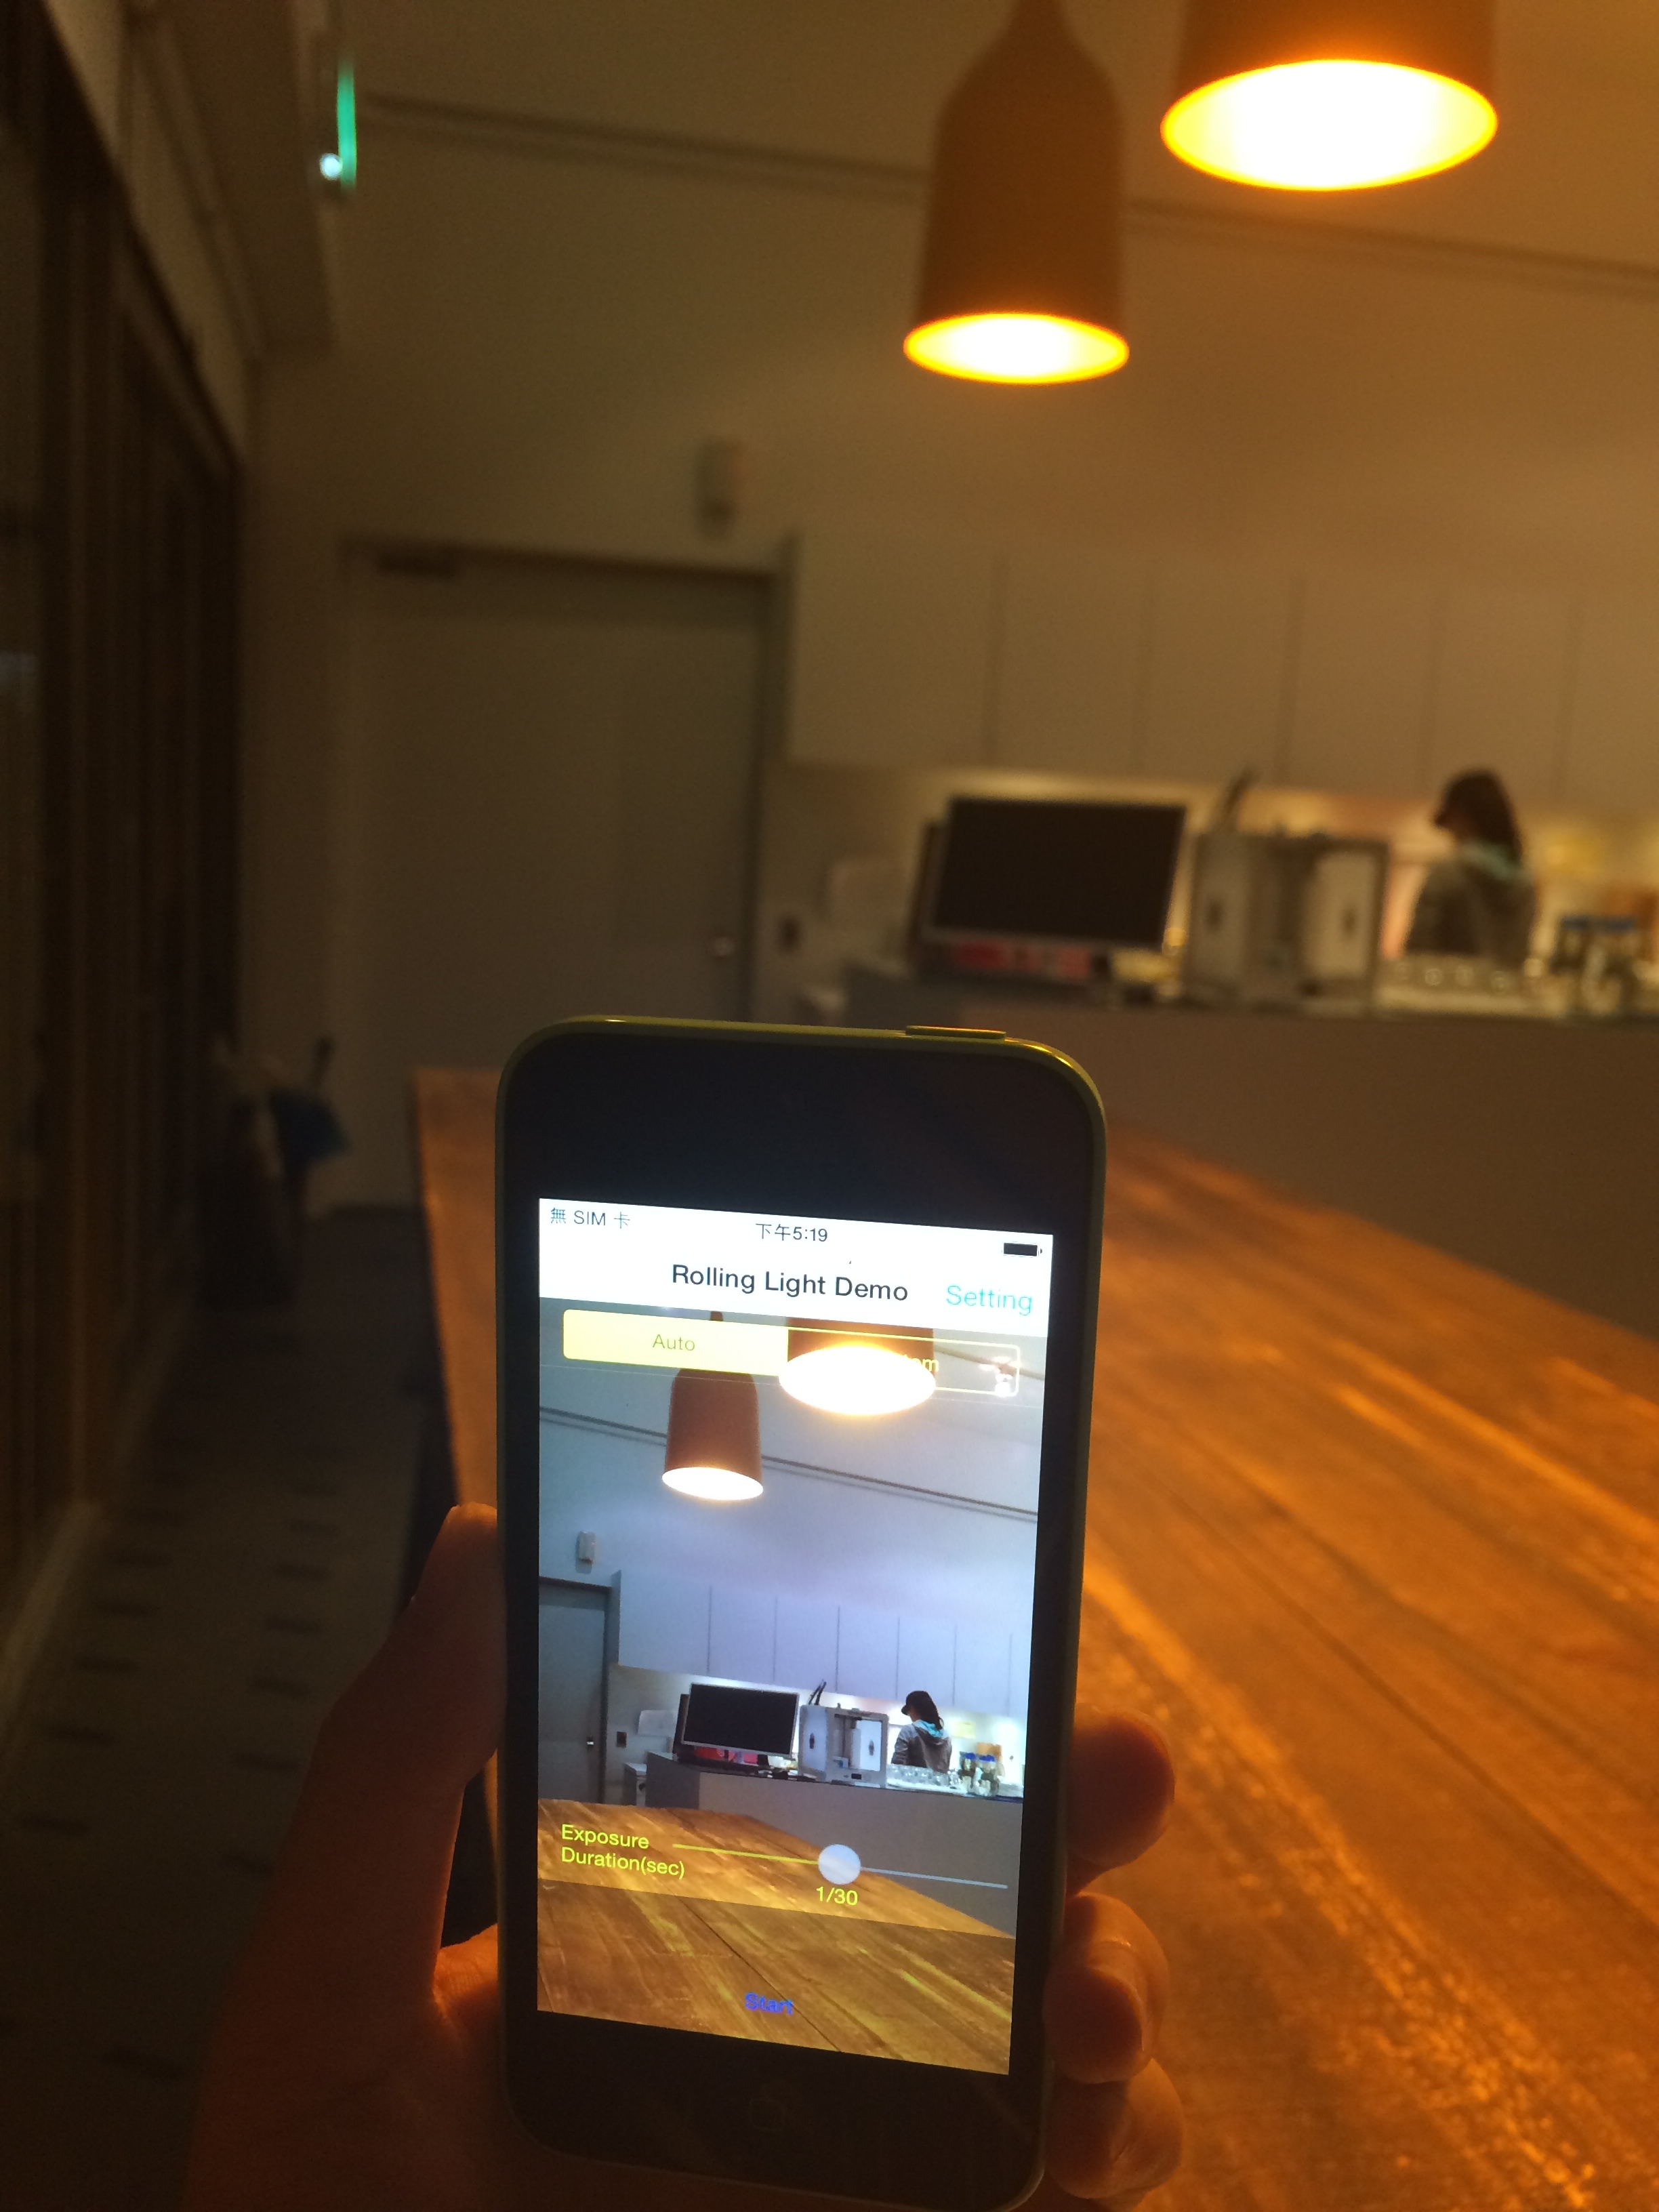
\includegraphics[scale=0.075]{pic/scenario.JPG}
	\centering
	\caption{An example of utilizing CamCom for visual association.}
	\label{fig:scenario}
\end{figure}

% Challenge 1:
% sync (repetitive signal does need to deal with it because data is encoded in only a single image frame)
% NLOS: easy to fix sync, low signal sample loss prob., LOS: difficult: patterns are incontinuous
% so we have sync mechanism
Challenge 1:
sync (repetitive signal does need to deal with it because data is encoded in only a single image frame)
NLOS: easy to fix sync, low signal sample loss prob., LOS: difficult: patterns are incontinuous
so we have sync mechanism 
%to be modified...
As the transmitting light and the receiving camera are not synchronized, the transmitting frame rate and the receiving frame rate are not usually the same.
When the transmitting frame rate is higher than the receiving frame rate, there could be symbol loss.
When the transmitting frame rate is lower than the receiving frame rate, reception of redundant symbols is possible. 
Although no information is lost, the receiver still needs to detect the redundant symbol so that it can be dropped to obtained the correct symbol sequence.
A more common event when the transmitting frame duration and the receiving frame duration are different is that there could be multiple image areas each corresponding to a symbol. In other word, a mix of different symbols in a single received image frame. 
A mixed frame is a very common and periodic event.
Even when the transmitting and the receiving frame durations are very close to each other, mixed frames would be received because of the phase difference between transmitter and receiver.Therefore, in this paper we also present a scheme that can handle \textbf{unsynchronized} transmitter and receiver pairs. 

% Challenge 2:  compatibility + high data rate
% one-way communication, but we want a higher rate → rolling shutter sampling (FSK) → 1/t_r is sampling rate, but different for different cameras → Read-out-time estimation for compatibility among different cameras
% high data rate, two possibility (1) high symbol rate → this is not possible, as a large portion of signal samples can be lost (2) high dimension modulation (high number of kinds of symbols) → we need accurate and fast frequency estimation algorithm (YIN and variants, compared to FFT and general DIP results)
% (??) impact of exposure time: unfixable: we do measurement?
Challenge 2:  compatibility + high data rate
one-way communication, but we want a higher rate → rolling shutter sampling (FSK) → 1/tr is sampling rate, but different for different cameras → Read-out-time estimation for compatibility among different cameras
high data rate, two possibility (1) high symbol rate → this is not possible, as a large portion of signal samples can be lost (2) high dimension modulation (high number of kinds of symbols) → we need accurate and fast frequency estimation algorithm (YIN and variants, compared to FFT and general DIP results)
(??) impact of exposure time: unfixable: we do measurement? 
%to be modified...
In this work, we presented a \textbf{theoretical model} to describe the single-LED-to-rolling-shutter-camera channel. Furthermore, we proposed the \textbf{Rolling Shutter-Frequency Shift Keying (RS-FSK) modulation} and demonstrated that the modulation is compatible to a wide range of CMOS cameras with different resolution, read-out time, and exposure time, satisfies the lighting requirements, and can be implemented with cost-efficient hardware. 

% ¶ para last - paper arrangements (optional) 
%to be modified... or not going to use
This paper proceeds as follows.
Chapter 2 presents some prior research done in this area.
Chapter 3 provides the background of the channel model of the rolling shutter camera, and RS-FSK modulation and demodulation techniques.
Chapter 4 states the problem caused by unsynchronized transmitter and receiver pairs.
Chapter 5 presents the hardware component and the software design of our system.
Chapter 6 presents our experiment and evaluation results. 
Finally, chapter 7 gives the concluding remarks of this thesis. 


% \begin{figure}[!htb]
% 	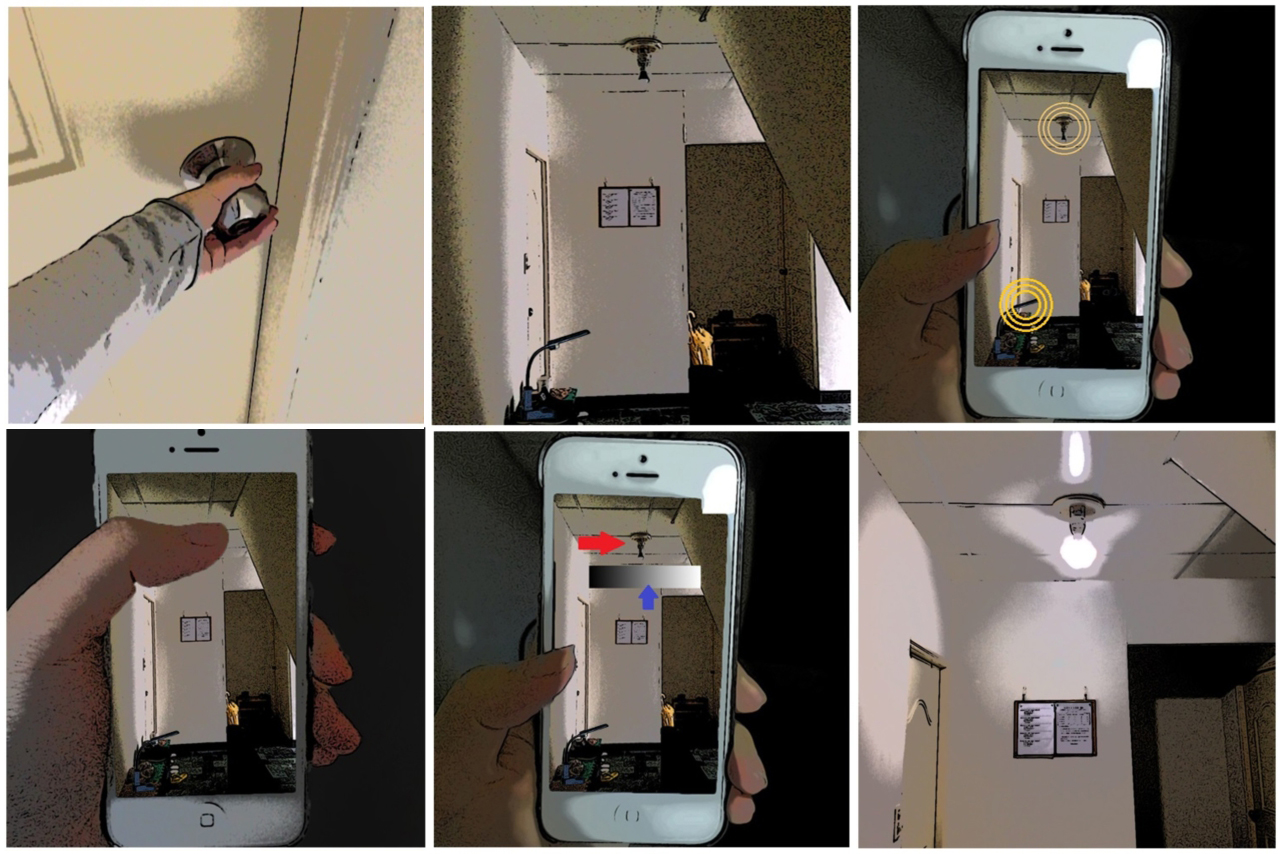
\includegraphics[scale=0.15]{fig/virtual_switch_hor.png}
% 	\centering
% 	\caption{An example of utilizing CamCom for visual association.}
% 	\label{fig:virtual_switch}
% \end{figure}

% Figure~\ref{fig:virtual_switch} shows a simple example. A user points her smartphone camera at multiple lights, touches the screen to select one, and uses the virtual switch that appears on the screen to adjust its lighting level. 
% In this scenario, the lights simply periodically transmit simple identifiers, such as IP addresses, to the smartphone. 
% The system is able to directly associate what the user sees (the image pixels mapped to the light selected by
% the user) to the transmission (the identifier of the light), and uses WiFi to sends the actual command to the right light to adjust the setting. 
% Compared to the conventional approach of identifying a particular set of visual features unique to the object with computer vision techniques, this approach is both simpler and more accurate.

% \begin{figure}[!htb]
% 	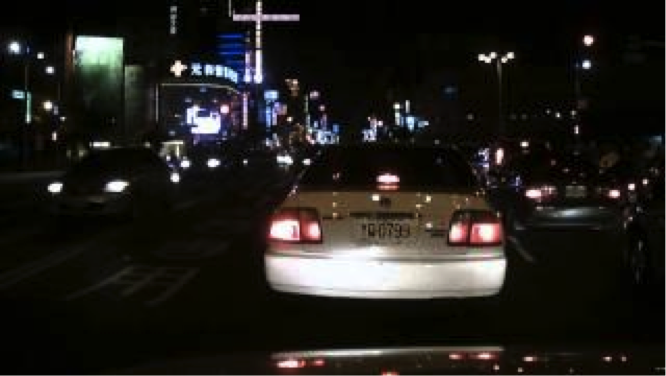
\includegraphics[scale=0.7]{fig/v2v.png}
% 	\centering
% 	\caption{An example of utilizing VLC for Vehicle communication.}
% 	\label{fig:v2v}
% \end{figure}
\section{related work}
	% -related work
	% 	-LOS vs NLOS (SNR實驗)
	% 	-communication not only localization
	% 	-luxapose
	% -rolling shutter相關知識
	% 	-operation and channel model
	% 	-特色:跟perspective, orientation無關

% \subsection{Camera-received VLC}
\subsection{Screen-to-camera Communications}
A number of prior works~\cite{perli2010pixnet,hao2012cobra,hu2013lightsync} utilized cameras as the receiver to implement one-way communication links. Those works utilized a LCD screen as the transmitter. The main benefit of this approach is that both the ability to display different colors and the high resolution of the LCD could be fully exploited, to improve the data rate.

PixNet \cite{perli2010pixnet} utilized the large quantity of pixels on a LCD to form OFDM symbols to transmit data to the camera receiver, and the implemented prototype has perspective correction ability.

COBRA \cite{hao2012cobra} proposed a similar approach that uses pixels as as barcodes and utilized the color information of pixels to achieve higher signal to noise ratio.
These works, however, did not solve the problems raised by the unsynchronized transmitter and receiver pair. The presented solution is to repeat the same packet transmission twice in order to guarantee the reception of all signal segments.

LightSync \cite{hu2013lightsync} introduces inter-frame erasure coding and line sequence number to reduce the high packet error rate due to synchronization issues. The approach also actively filters out rolling-shutter effects.

VRCodes (NewsFlash) \cite{vrcodes} takes advantage of the rolling shutter effect to decode visual tags displayed on LCDs. The tags use multiple pixels of different colors, modulated at up to 120Hz to transmit data. The technology exploits the "flicker-fusion threshold" of the human eye to blend the tags into the background by rapidly flashing complimentary hues of color, still visible to a rolling shutter camera. This work suggests how different color channels could be used to increase data throughput, while still keeping transmissions imperceptible to humans.

Visual MIMO \cite{visualmimo1, visualmimo2, visualmimo3} is a method that uses any light-emitting spatial array as the transmitter and uses ordinary cameras as the receivers.
It proposes a photometric modeling for hidden imagery and can realize a dual use of the electronic display: to display an image for human observation while simultaneously transmitting hidden bits for decoding by a camera.

Compared to these works, we proposed to use only a single LED light as the transmitter and a commonly available CMOS camera as the receiver, and many design considerations are not the same as these prior research works utilizing multiple optical transmitting sources.

\subsection{Single-LED-to-camera Communications}
Three works \cite{roberts2013undersampled, danakis2012using,landmark} have previously investigated how to implement single-LED-to-camera communication links. 
In~\cite{roberts2013undersampled}, the author proposes undersampled frequency shift OOK (UFSOOK), which allows the use of a high signal frequency while the modulation can still be decoded by a common camera with 30 fps (frame rate per second). The scheme is compatible to both global shutter and rolling shutter cameras, but the maximum achievable data rate is only half of the frame rate per light source.

In \cite{danakis2012using}, the authors utilized rolling shutter sampling to encode data with Manchester coding at high symbol rate, and was the first work to take advantage of the rolling shutter to implement CamCom. 
However, the implementation exhibits a high packet drop rate due to the long processing time of the decoder application per frame and lack of considerations for synchronization issues. Thus, the reception is not continuous and some frames are inevitably lost. The transmitter then needs to send signal.
In addition, the transmitting light needs to illuminate the entire image for the receiver to demodulate the transmission.We can achieve a data rate much higher than 50\% of the frame rate per light source, and have designs to address the issues caused by the exposure operation of the camera and unsynchronized nature of the communication link.
A further drawback in this work is that the modulated signal can produce a human perceivable flicker from transmitting LED. The authors alleviate this by imposing a DC bias on the signal, which in turn decreases its dynamic range and SNR at the receiver. This makes the scheme require significantly brighter lights and more complex driving hardware than our proposed approach.

In \cite{landmark}, the author used binary frequency shift keying (BFSK) of a high frequency PWM signal to encode data that can be used as localization landmarks. On the receiver side, they exploited rolling shutter camera sensors to detect high-frequency changes in the intensity of light reflected off surfaces, which is indirect line-of-sight of the camera. The data rate is only 1.25 bytes per second (the authors claimed that it is fast enough to send an ID code) while in our work there is a need to increase the data rate to communicate rather than just perform localization. To detect the transmitting frequency, they used 1-D fast Fourier transform. However, we have tried the FFT method before and it usually requires a threshold to eliminate the noise. It is hard to have a general threshold which can be adopted in different environments. For the receiver which is unsynchronized with the transmitter, they proposed a sliding window approach where they first stitch all of the captured frames together into a single, long image. Then they can detect the frequency by sliding the window and locating the window position corresponding to the highest power. However, we can stitch the images only if the light is full of whole image (for example, reflected from the surface). Moreover, if there is a symbol loss between the two frames, then the result of stitching images would likely be inaccurate. In our work, we use additional schemes to address these problems.
\section{CHALLENGES \& SYSTEM OVERVIEW}
%-challenge
%-流程圖
test intro
\section{RollingLight design}

\section{CHALLENGES \& SYSTEM OVERVIEW}
%-challenge
%-流程圖
test intro
\begin{figure}[!t]
  \centering
  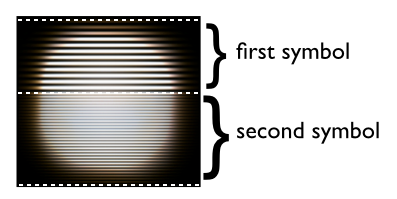
\includegraphics[scale=0.4]{pic/mixed_frame.png}
  \caption{Received frame with mixed symbols.}
  \label{fig:mix_photo}
\end{figure}

\begin{figure}[!t]
  \centering
  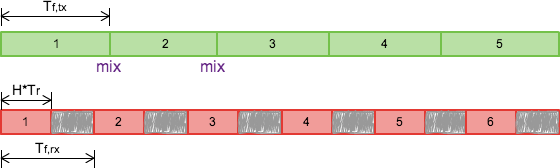
\includegraphics[scale=0.35]{fig/mix2.png}
  \caption{Mixed frame illustration.}
  \label{fig:mix2}
\end{figure}

\subsection{Parity Symbol and Sequence Number}
To deal with the unsynchronized problem, we add additional schemes.
The sequence number is used to identify any missing symbol or redundant symbol. Missing symbols will be reconstructed with corresponding parity symbols, while redundant symbols with the same sequence number will be dropped.

As symbols could be lost or corrupted due to the time gap of the channel or if the exposure time is an integer multiple of the signal period,
a parity symbol is inserted for every $n$ data symbols by \textbf{XOR-ing} all $n$ data symbols, so that if only one of the $n$ data symbols or the parity symbol is not correctly received, the receiver can \textbf{recover the lost symbol}. The number of parity symbols that should be added to a packet can be determined by calculating expected number of lost symbols in a packet using the probability equation in \autoref{sec:unsync}. 

After constructing a sequence of symbols, including the parity symbol, to be transmitted, we label each symbol with a \textbf{1.5 bit} sequence number $=\{0,1,2\}$.
The sequence number can be obtained by calculating the index number modulo 3.
The sequence number is then combined with the data symbol to become one meta symbol, then mapped to one of the selected signal periods.
Note that the sequence number reduces the number of bits that can be represented by each symbol by 1.5 bits. However, this is required to detect \textbf{lost symbols} (when the transmitting frame duration is smaller than the receiving frame duration) or \textbf{redundant symbols} (when the transmitting frame duration is larger than the receiving frame duration).
Taking the assumption into consideration, it can be proved that there could be no consecutive symbol losses. Thus, a 1.5 bit sequence number, $\{0,1,2\}$, would be sufficient determine the location of a lost symbol in the sequence. 
% Note that the sequence number will be represented by the most significant 1.5 bits in a symbol, i.e., symbols with different sequence numbers will be separated with a large margin, and thus getting an erroneous sequence number is unlikely. \\
% The sequence number is used to identify any missing symbol or redundant symbol. Missing symbols will be reconstructed with corresponding parity symbols, while redundant symbols with the same sequence number will be dropped. In the case that redundant symbols with the same sequence number is demodulated to different symbols, the one decoded with the largest image area will be used.

\begin{figure}[!t] %move forward
  %\centering
  \hspace{-1em}
  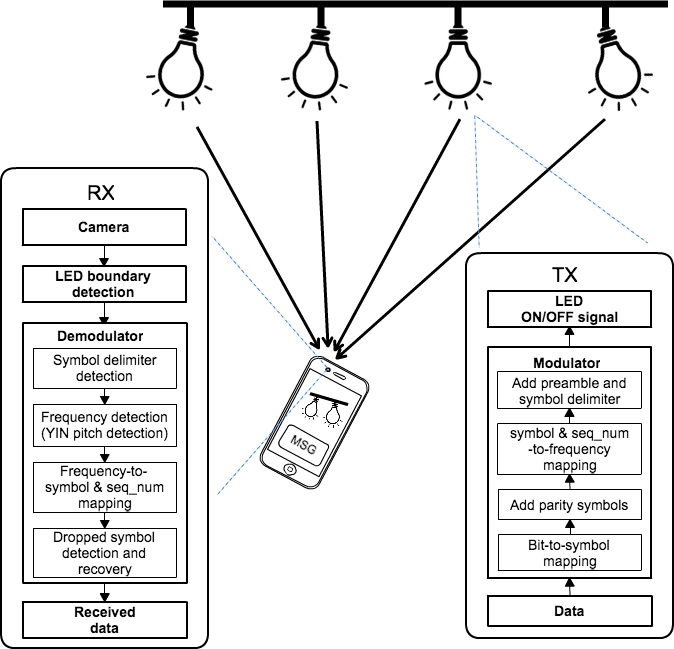
\includegraphics[scale=0.375]{pic/arch.png} 
  \caption{System Architecture of RollingLight}
  \label{fig:SystemArchitecture}
\end{figure}

\subsection{Preamble Symbol} 
The preamble symbol, which has a signal period known to the receiver, is inserted at the beginning of the symbol sequence.
The preamble symbol serves two functions: one is for the receiver to detect the start of the packet and start the subsequent demodulation process, while the other is for the receiver to accurately \textbf{calibrate its $T_r$ value} based on the period estimate of the preamble, so that the error of the period estimates of all subsequent symbols in this packet can be minimized. As a result, the signal period with the smallest error variation is selected as the period for the preamble symbol. %In our experiment, we select the 5657.3886 Hz as the period for the preamble symbol. This is the highest frequency used in our design. 

\subsection{Symbol Delimiter}
% Finally, another signal period is selected as the symbol delimiter signal period.
This scheme is also for addressing the unsynchronized issue.
We select another signal period as the symbol delimiter.
In order to easily \textbf{separate consecutive symbols} in the same image, i.e., two areas in the image showing signals with different periods, a signal with this signal period will be transmitted for a short duration between any two symbol transmissions as \autoref{fig:FD} shows. 

\begin{figure}[!t]
  \centering
  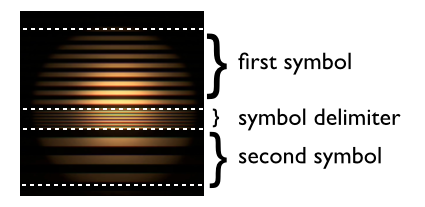
\includegraphics[scale=0.4]{pic/symbol_delimiter.png} 
  \caption{Symbol delimiter illustration.}
  \label{fig:FD}
\end{figure}

\begin{figure*}[!t]
   \centering
   \begin{subfigure}[h]{0.16\textwidth}
      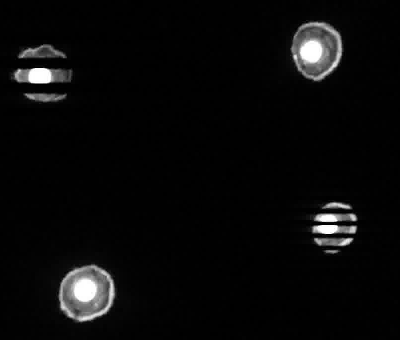
\includegraphics[width=\textwidth]{pic/bbox/bbox_A_original_crop.png}
      \caption{Original} \label{fig:bbox_ori}
   \end{subfigure}%
   ~
   \begin{subfigure}[h]{0.16\textwidth}
      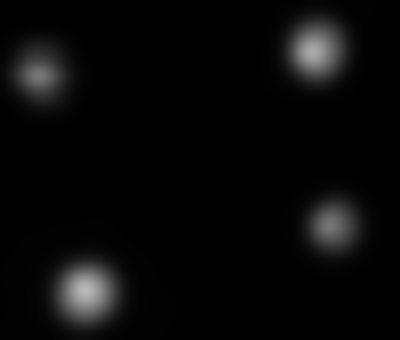
\includegraphics[width=\textwidth]{pic/bbox/bbox_B_gaussianBlur_crop.png}
      \caption{Gaussian Blur} \label{fig:bbox_blur}
   \end{subfigure}%
   ~  
   \begin{subfigure}[h]{0.16\textwidth}
      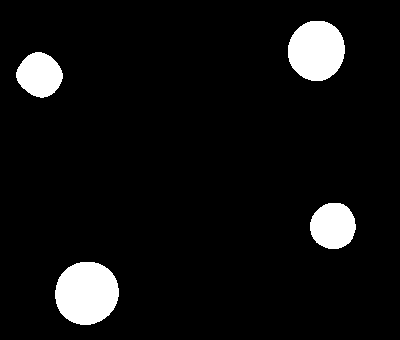
\includegraphics[width=\textwidth]{pic/bbox/bbox_C_OTSU_crop.png}
      \caption{Binary OTSU} \label{fig:bbox_otsu}
   \end{subfigure}%
   ~
   \begin{subfigure}[h]{0.16\textwidth}
      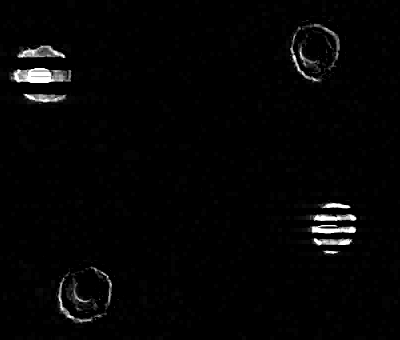
\includegraphics[width=\textwidth]{pic/bbox/bbox_E_template_crop.png}
      \caption{Template} \label{fig:bbox_template}
   \end{subfigure}%
   ~
   \begin{subfigure}[h]{0.16\textwidth}
      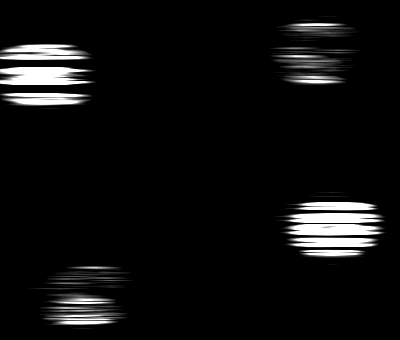
\includegraphics[width=\textwidth]{pic/bbox/bbox_F_haar_crop.png}
      \caption{Haar-like Feature} \label{fig:bbox_haar}
   \end{subfigure}%
   ~   
   \begin{subfigure}[h]{0.16\textwidth}
      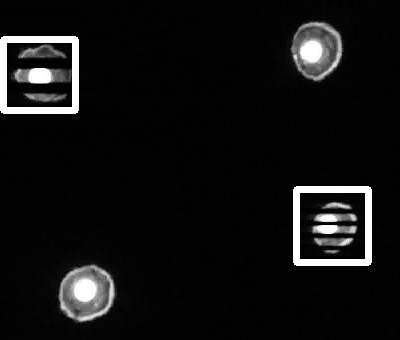
\includegraphics[width=\textwidth]{pic/bbox/bbox_H_stripedLED_crop.png}
      \caption{Result} \label{fig:bbox_result}
   \end{subfigure}%
   \\
   \begin{subfigure}[h]{0.16\textwidth}
      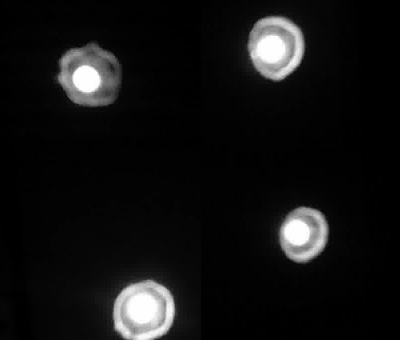
\includegraphics[width=\textwidth]{pic/bbox/bbox_A_original400_crop.png}
      \caption{Original} \label{fig:bbox_ori}
   \end{subfigure}%
   ~
   \begin{subfigure}[h]{0.16\textwidth}
      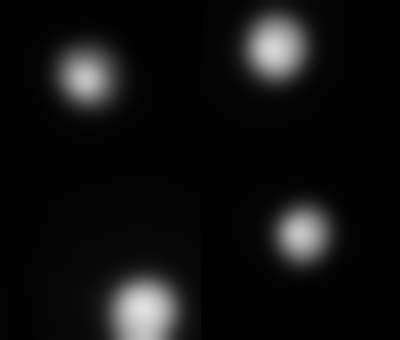
\includegraphics[width=\textwidth]{pic/bbox/bbox_B_gaussianBlur400_crop.png}
      \caption{Gaussian Blur} \label{fig:bbox_blur}
   \end{subfigure}%
   ~  
   \begin{subfigure}[h]{0.16\textwidth}
      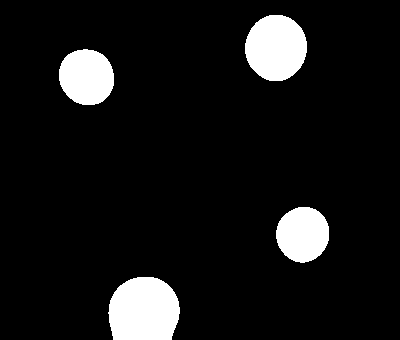
\includegraphics[width=\textwidth]{pic/bbox/bbox_C_OTSU400_crop.png}
      \caption{Binary OTSU} \label{fig:bbox_otsu}
   \end{subfigure}%
   ~
   \begin{subfigure}[h]{0.16\textwidth}
      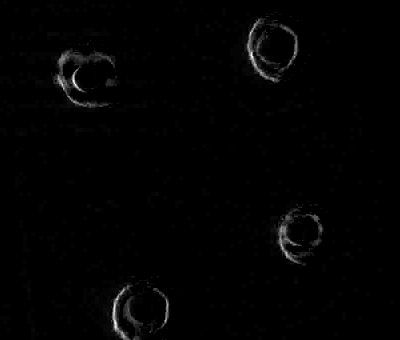
\includegraphics[width=\textwidth]{pic/bbox/bbox_E_template400_crop.png}
      \caption{Template} \label{fig:bbox_template}
   \end{subfigure}%
   ~
   \begin{subfigure}[h]{0.16\textwidth}
      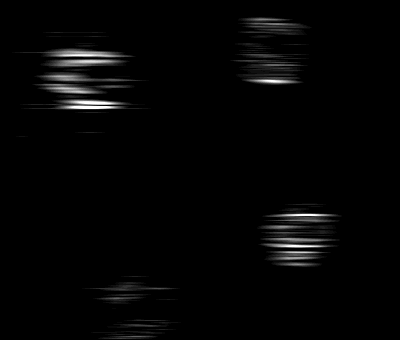
\includegraphics[width=\textwidth]{pic/bbox/bbox_F_haar400_crop.png}
      \caption{Haar-like Feature} \label{fig:bbox_haar}
   \end{subfigure}%
   ~   
   \begin{subfigure}[h]{0.16\textwidth}
      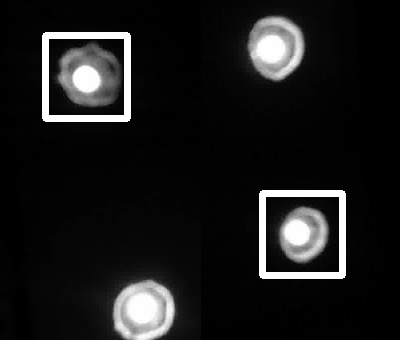
\includegraphics[width=\textwidth]{pic/bbox/bbox_H_stripedLED400_crop.png}
      \caption{Result} \label{fig:bbox_result}
   \end{subfigure}%
   \caption{LED boundary detection step-by-step. The top row of images taken with exposure duration 1/5000 sec. The bottom row of images taken with exposure time 1/400 sec. The result image detects the light with strips.}
   \label{fig:bbox}
\end{figure*}

The detection step is done by calculating the value of the difference function described in \autoref{sec:demodulation} for all possible symbol delimiter locations in the image, but only with a fixed shift value that equals the the signal period of the symbol delimiter. If the minimum value of the function for all possible delimiter locations is larger than a pre-defined threshold, then it will output the location of the symbol delimiter.

\subsection{LED Boundary Detection}
To decode the lights, the first step is to find the boundary of each light in the received image.We follow the~\cite{luxapose} to detect the lights individually. We slightly modified the detection process. To detect the light taken with larger exposure duration, we need to eliminate the background noise. Our method is maintain a buffer with latest few images, for the current image, we make a template by averaging all images in the buffer. Then we subtract the template from the current image to eliminate the noise. Another modification is the haar-like feature. Since there would be some other light in the image, we want to further detect the modulated light, that is, the light with strips. Thus the haar-like feature is added to filter the light with strips.

~\autoref{fig:bbox} shows the light detection process step-by-step. There are four lights, two of them (the top-left and the bottom-right one) are modulated. We test the detection method with two exposure time settings: the larger one 1/400 sec and the smaller one 1/5000 sec.
More sophisticated detection and tracking algorithms based on computer vision techniques can be utilized if necessary.

% \textbf{Bit-to-symbol mapping.} Data bits to be transmitted will first be split into bit patterns of a constant length. Each bit pattern is then mapped to a data symbol. \\

% \textbf{Parity symbol.} As symbols could be lost or corrupted due to the time gap of the channel or if the exposure time is an integer multiple of the signal period,
% a parity symbol is inserted for every $n$ data symbols by \textbf{XOR-ing} all $n$ data symbols, so that if only one of the $n$ data symbols or the parity symbol is not correctly received, the receiver can \textbf{recover the lost symbol}. The number of parity symbols that should be added to a packet can be determined by calculating expected number of lost symbols in a packet using the probability equation in \autoref{sec:unsync}. \\ 

% \textbf{Sequence number.} After constructing a sequence of symbols, including the parity symbol, to be transmitted, we label each symbol with a \textbf{1.5 bit} sequence number $=\{0,1,2\}$.
% The sequence number can be obtained by calculating the index number modulo 3.
% The sequence number is then combined with the data symbol to become one meta symbol, then mapped to one of the selected signal periods.
% Note that the sequence number reduces the number of bits that can be represented by each symbol by 1.5 bits. However, this is required to detect \textbf{lost symbols} (when the transmitting frame duration is smaller than the receiving frame duration) or \textbf{redundant symbols} (when the transmitting frame duration is larger than the receiving frame duration).
% Taking the assumption into consideration, it can be proved that there could be no consecutive symbol losses. Thus, a 1.5 bit sequence number, $\{0,1,2\}$, would be sufficient determine the location of a lost symbol in the sequence. 
% Note that the sequence number will be represented by the most significant 1.5 bits in a symbol, i.e., symbols with different sequence numbers will be separated with a large margin, and thus getting an erroneous sequence number is unlikely. \\

% \textbf{Preamble symbol.} Next, the preamble symbol, which has a signal period known to the receiver, is inserted at the beginning of the symbol sequence.
% The preamble symbol serves two functions: one is for the receiver to detect the start of the packet and start the subsequent demodulation process, while the other is for the receiver to accurately \textbf{calibrate its $T_r$ value} based on the period estimate of the preamble, so that the error of the period estimates of all subsequent symbols in this packet can be minimized. As a result, the signal period with the smallest error variation is selected as the period for the preamble symbol. In our experiment, we select the 5657.3886 Hz as the period for the preamble symbol. This is the highest frequency used in our design. \\

% \textbf{Symbol delimiter.} Finally, another signal period is selected as the symbol delimiter signal period.
% In order to easily \textbf{separate consecutive symbols} in the same image, i.e., two areas in the image showing signals with different periods, a signal with this signal period will be transmitted for a short duration between any two symbol transmissions. %as Figure~\ref{fig:FD} shows. 
% The transmitting light is then driven to transmit a sequence of square waves according to pre-determined list of signal periods representing the entire data packet. \\

% \begin{figure}[!t]
%   \centering
%   \includegraphics[scale=0.8]{fig/fd.png} 
%   \caption{Frame delimiter illustration. The upper shows the frame without frame delimiter; the lower shows the frame with frame delimiter.}
%   \label{fig:FD}
% \end{figure}

% \begin{figure}[!t]
%   \centering
%   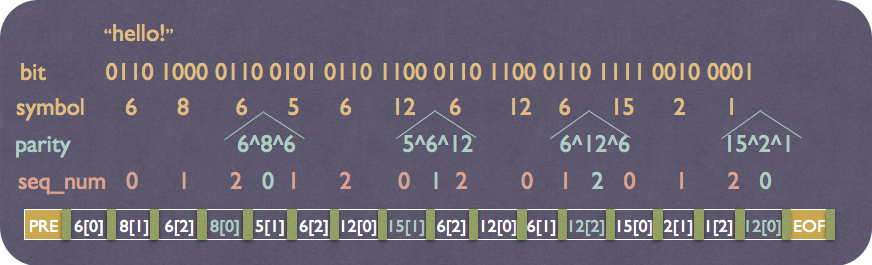
\includegraphics[scale=0.25]{fig/flow_tx.png} 
%   \caption{An example flow of the transmitter end.}
%   \label{fig:flow_tx}
% \end{figure}

% \autoref{fig:flow_tx} shows an example flow of the transmitter end. The message "hello!" is converted to the bit string, Then every 4-bit is mapped to a symbol. Assume the $P_{miss}$ is 0.25, which means a parity symbol is inserted for every 3 symbols. Next step we tag the symbols (including parity symbol) in the order of $\{0,1,2\}$ as the sequence number. The last step is to add the preamble symbol and the EOF symbol (the yellow part in the figure) at the beginning and the end of the data, and the symbol delimiter symbol (the green part in the figure) between each data symbols. 

% \textbf{LED boudary detection.} The receiving camera captures a series of images with the transmitting light. The receiver starts the demodulation process by determining the image area occupied by the transmitting light. In our system, this is done by extracting an area with very high intensity values. More sophisticated detection and tracking algorithms based on computer vision techniques can be utilized if necessary. \\

% \textbf{Symbol delimiter detection.}
% A symbol delimiter detector is then executed to determine whether a symbol delimiter area presents in the image. 
% % \autoref{fig:flow_rx} shows the received image which contains a symbol delimiter. 
% The detection step is done by calculating the value of the difference function described in \autoref{sec:demodulation} for all possible symbol delimiter locations in the image, but only with a fixed shift value that equals the the signal period of the symbol delimiter. If the minimum value of the function for all possible delimiter locations is larger than a pre-defined threshold, then it will output the location of the symbol delimiter. Then, the period detection algorithm can be executed to determine the signal periods of two image areas separated by the symbol delimiter. In this case, the signal periods of both symbols can be accurately estimated.

% % \begin{figure}[!t]
% %   \centering
% %   \includegraphics[scale=0.25]{fig/FD_illustration} 
% %   \caption{Received frame with frame delimiter.}
% %   \label{fig:FD_photo}
% % \end{figure}
% % \begin{figure}[!t]
% %   \centering
% %   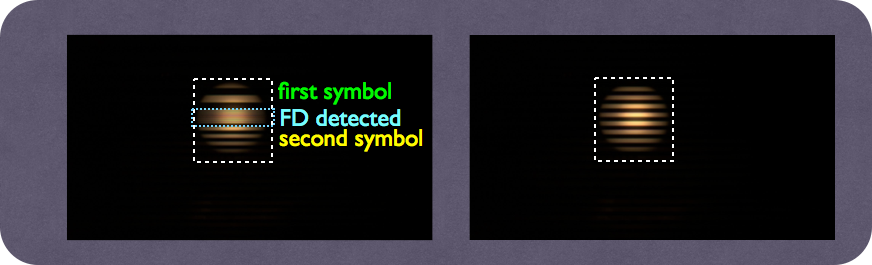
\includegraphics[scale=0.25]{fig/flow_rx.png} 
% %   \caption{An example flow of the symbol delimiter detection of the receiver end.}
% %   \label{fig:flow_rx}
% % \end{figure}

% The estimated signal period will be mapped to a meta symbol. The meta symbol is then split into a sequence number and a data symbol. \\

% \textbf{Dropped symbol detection and recovery.}
% Then, the sequence number is used to identify any missing symbol or redundant symbol. Missing symbols will be reconstructed with corresponding parity symbols, while redundant symbols with the same sequence number will be dropped. In the case that redundant symbols with the same sequence number is demodulated to different symbols, the one decoded with the largest image area will be used.

% The data string is finally obtained after mapping the sequence of data symbols back to the bit patterns, forming the original bit stream.

\section{Implementation}

	% -介紹device跟implement細節
	% -說明real-time(列出time)

\subsection{Components}

% \begin{figure}[!t]
%   \centering
%   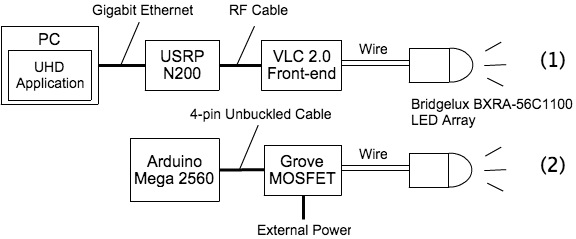
\includegraphics[scale=0.4]{pic/tx_devices.png} 
%   \caption{Transmitter Components}
%   \label{fig:tx_component}
% \end{figure}
% \begin{figure}[!t]
%   \centering
%   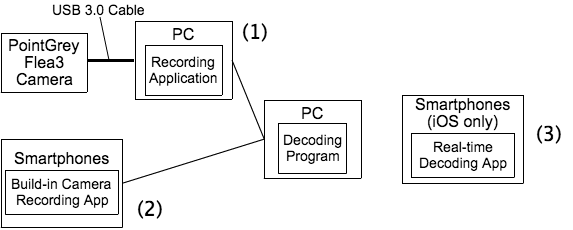
\includegraphics[scale=0.4]{pic/rx_devices.png} 
%   \caption{Receiver Components}
%   \label{fig:rx_component}
% \end{figure}

% As the system is still under development, the developed system should be sufficiently flexible so that it is easy to change various desires of the system, e.g., the modulation format, the protocol design, etc. 
% To this end, we utilize a software-defined radio (SDR) platform in our system, which enables us to make most necessary modifications in software with minimal efforts. 
% Additional hardware components were developed to interface between the SDR and the optical transmitting and receiving components. \\
% \autoref{fig:tx_component} shows the transmitter components in our proposed VLC system. 

\autoref{fig:components} shows the components in our proposed system. 
In the transmitting end, we use two different architectures to modulate the LED.
First, as the system is still under development, the developed system should be sufficiently flexible so that it is easy to change various desires of the system, e.g., the modulation format, the protocol design, etc. To this end, we use a PC with USRP Hardware Driver (UHD) application to modulate the digital information in a packet into analog signal, in the format of digitized samples. 
The software-defined radio (SDR) is connected to the PC via Gigabit Ethernet. The SDR converts the digitized samples sent from the PC into analog signal. 
The VLC 2.0 front-end board converts the voltage varying signal to current varying signal and outputs that to the LED. The signal would determine the output intensity of the LED. 

In the next stage, we try to minimize the cost of the transmitter. We use the Arduino Mega 2560 board instead, and we use Grove MOSFET which enable us to control higher voltage project, say 15VDC, with low voltage, say 5V, on microcontroller. 

In the receiving end, we just use a camera to receive the optical signal and use simple computer vision and digital image processing mechanism to demodulate. Again, we have different architectures.
First, we use PointGrey Flea3 camera~\cite{pointgrey_flea}, a high-speed camera built for experimental purposes, thus various parameters such as exposure time can be adjusted to a wide range of values. This allows us to examine system performance in different conditions. 

We also use a number of smartphones to compare their performance. We take the videos from the built-in camera app, then decoding the video on PC.

The third architecture, ideally, is to decode the preview images on the smartphone directly without storing a video and decoding at external machine. We developed an iOS app. 

% \begin{figure}[!t]
% \centering
%  \begin{subfigure}[h]{0.1\textwidth}
%   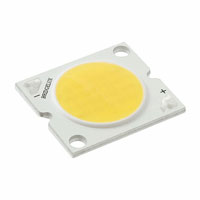
\includegraphics[width=\textwidth]{fig/LED_array.jpg} 
%   \caption{Bridgelux BXRA-W0802 LED Array} \label{fig:led_array}
%  \end{subfigure}
% ~
%  \begin{subfigure}[h]{0.1\textwidth}
%   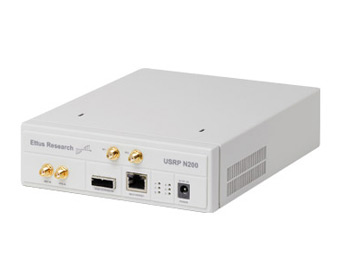
\includegraphics[width=\textwidth]{fig/usrp.jpg} 
%   \caption{USRP N200 Software Defined Radio} \label{fig:usrp}
%  \end{subfigure}
% ~
%  \begin{subfigure}[h]{0.1\textwidth}
%   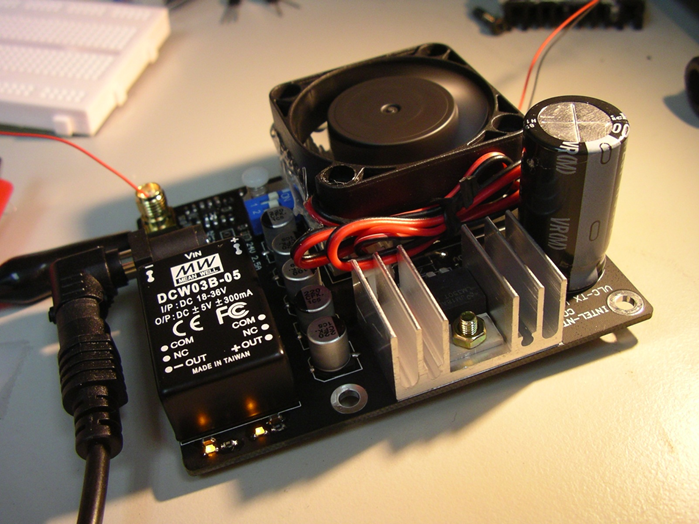
\includegraphics[width=\textwidth]{fig/VLC2_0.png} 
%   \caption{VLC 2.0 Front-end Board} \label{fig:VLC_frontend}
%  \end{subfigure}
% \caption{Photos of Transmitter Components}
% \label{fig:tx_photo}
% \end{figure}

% \begin{figure}[!t]
% \centering
%  \begin{subfigure}[h]{0.2\textwidth}
%   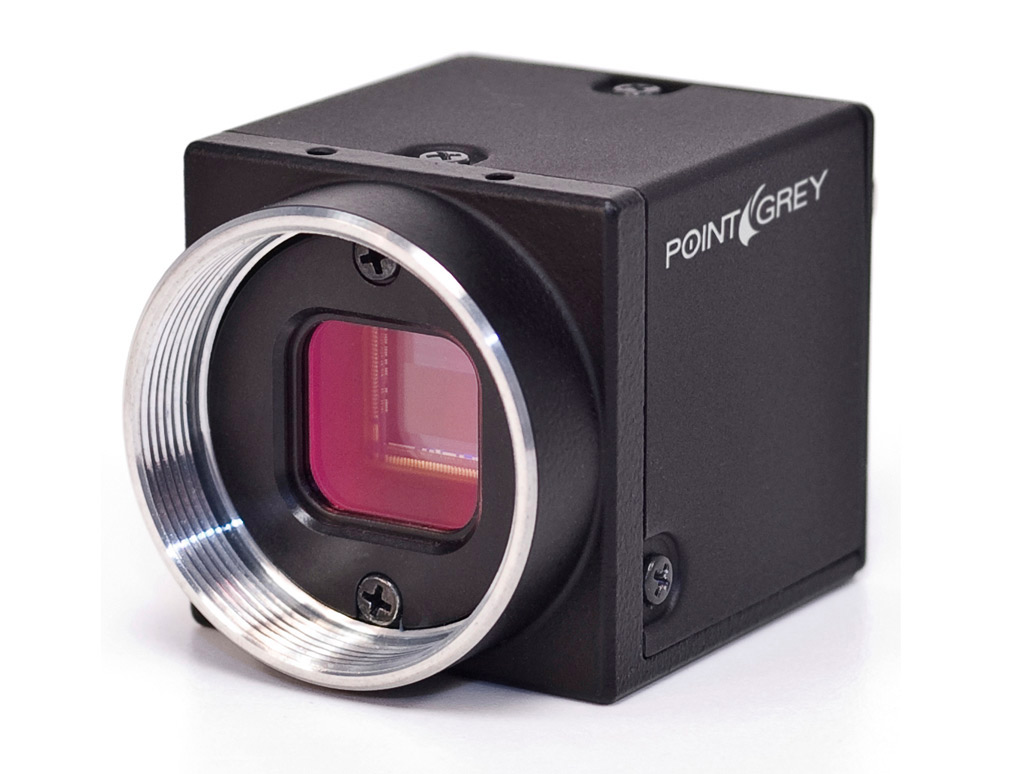
\includegraphics[width=\textwidth]{fig/flea3.jpg} 
%   \caption{PointGrey Flea3 Camera} \label{fig:flea}
%  \end{subfigure}
% ~
%  \begin{subfigure}[h]{0.2\textwidth}
%   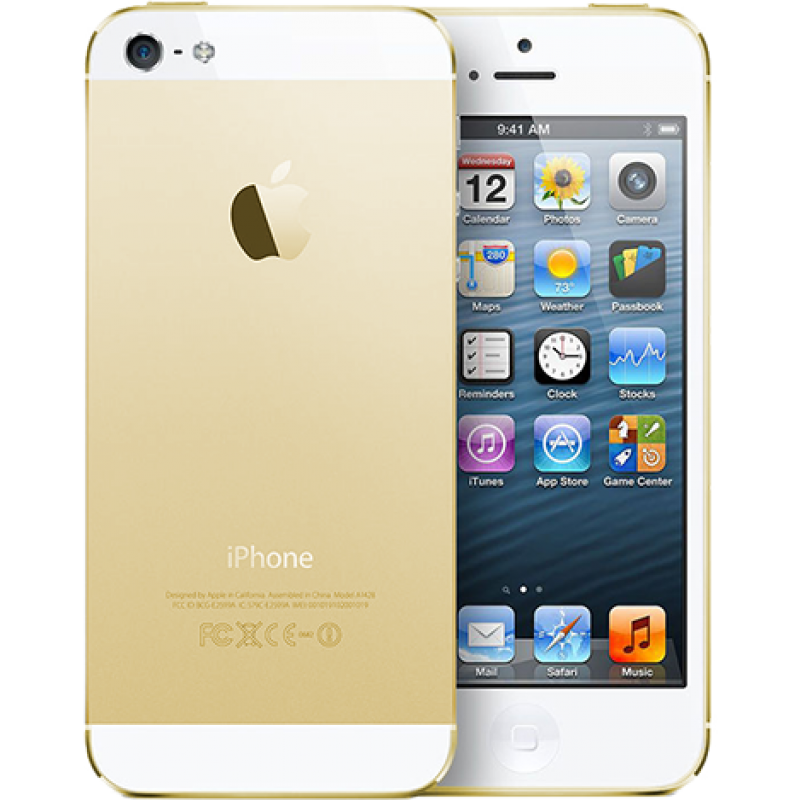
\includegraphics[width=\textwidth]{fig/iphone5s.png} 
%   \caption{SmartPhone Camera (iPhone5S)} \label{fig:iphone5s}
%  \end{subfigure}
% \caption{Photos of Receiver Components}
% \label{fig:rx_photo}
% \end{figure}

% In the following, we will describe the components in the system in detail.
% \subsubsection{LED Array}
% \autoref{fig:led_array} shows the Bridgelux BXRA-W0802~\cite{Bridgelux}, which is a high brightness LED array suitable for indoor illumination purposes and chosen as the transmitting LED component. The maximum DC forward current is 2 amps, and the typical forward voltage is around 13 volts, resulting in a maximum output power of 26 W. Typical luminous flux with 1050 mA forward is 850 lumen.

% \subsubsection{Software Defined Radio}
% As a highly flexible tool to realize the traditional RF communications, SDR has become our preferred platform to develop the VLC system. In our system, we use Ettus Universal Software Radio Peripheral (USRP) N200, as \autoref{fig:usrp} shows. USRP then converts the digital signal samples to analog voltage-varying signal.
% The unit features a gigabit ethernet interface to transfer signal samples to the PC. 
% N200 provides high-bandwidth and high-dynamic range processing capability. 
% A modular design allows the N200 to operate from DC to 6 GHz. 

% In our system we use a daughter board (LFTX) that is capable of transmitting signals from DC to 30 MHz. 
% N200 can stream up to 50 MegaSample/s to and from host applications, and users can implement custom functions in the FPGA fabric, or in the on-board 32-bit RISC softcore. The FPGA offers the potential to process up to 100 MHz of RF bandwidth in both the transmit and receive directions. 
% This is more than sufficient for our application as VLC usually operates in the range of 0.1 kHz to several kHz. The sampling rate to convert the digital samples to analog signal is configured at 1 MHz. This could emulate the clock rate of a low-cost microcontroller. Inaccuracy in the transmitted signal period could be caused by low sampling rate.

% \subsubsection{UHD}
% UHD is a driver developed by Ettus Research and is compatible with all USRP software-defined radios. 
% UHD allows development on multiple operating systems.
% UHD provides an application programming interface (API), which provides access to various functions of the USRP including synchronization, sample streaming, and configuration. 

% In the thesis, we modify one of the example applications provided with the UHD software package to modulate the transmitting signals.

% \subsubsection{VLC Front-end Board}

% The output light intensity of the LED depends on the magnitude of the input current. Thus, a hardware component is required to interface between the SDR and the LED component, linearly converting a voltage-varying signal to a current-varying signal. We utilize a custom-made VLC front-end circuit board, as shown in \autoref{fig:VLC_frontend}. 

% One of the main objectives for the design of the front-end board is to accurately convert the level of voltage in the input signal to the level of the output intensity of the attached LED. 
% For example, when the voltage of input signal is zero, the front-end would control the light intensity of the LED to be zero, and when the voltage of the input signal is raised to the maximum, the light intensity of the LED should also at its maximum. 

% Moreover, this conversion also needs to be done fast enough so that a high frequency signal can be transmitted. 

% \subsubsection{Rolling Shutter Camera}
% There are a number of cameras used in our experiments. 
%  \autoref{fig:flea} shows the specification of PointGrey Flea3 (FL3-U3-88S2C-C)~\cite{pointgrey_flea}, a high-speed camera built for experimental purposes, thus various parameters such as exposure time can be adjusted to a wide range of values. This allows us to examine system performance in different conditions. 
%  %\autoref{tab:flea_spec} lists the specification of Point Grey Flea3 camera.

% The cameras on smartphones, such as HTC New One and iPhone 5S shown in \autoref{fig:iphone5s} , are also selected for some experiments, in order to determine the expected performance of RS-FSK on cameras in off-the-shelf smartphones. 

% \begin{table}[!t]
% \centering
% \caption{Specification of Point Grey Flea3 (FL3-U3-88S2C-C).}
%   %\large
% 	\begin{tabular}{lc}
%   \hline Parameter & Value \\
%   \hline 
% 	\hline Camera Sensor Format & 1/2.5" \\
% 	\hline Type of Sensor & Sony IMX121 CMOS \\
% 	\hline Pixel (H x V) & 4096 x 2160, 2048 x 1080 \\
% 	\hline Pixel Size (H x V) & 1.55$\mu$m x 1.55 $\mu$m \\
% 	\hline Max Frame Rate (fps) & 21.6, 60 \\
% 	\hline Type of Shutter & Rolling Shutter \\
% 	\hline Exposure Time & 0.015 ms - 1 s \\
% 	\hline Estimated Read-out Time & 0.01473 ms \\
%   \hline 
% 	\end{tabular}
% 	\label{tab:flea_spec} 
% \end{table}

\subsection{Encoder} 
For the transmitting end of the system, we implement a UHD application to generate the signal. It takes a given bit stream, and produces encoded frames following a predefined bit-to-symbol mapping and the frame layout described in the previous subsection. We use 1 MHz sampling rate and a given transmitting frame rate to generate samples within one frame. These samples are then encoded with bit 1s and 0s with the corresponding symbol frequency.
The frames are then turned into analong signal and transmitted via LED light.

For another architecture, we use the Fast PWM with OCRnA top mode and the interrupt mechanism to control the clock of the Microcontroller of the Arduino Mega board. We can set the symbol frequency, the duty cycle, and the symbol duration.

\subsection{Decoder} 
We use the ffmpeg package to convert video into image frames. The decoder is implemented with OpenCV, which is a very powerful and efficient library to process images.
%The decoder is implemented in several programming languages. Two are implemented in Matlab and C++ with OpenCV for post processing and analyzing. 
The other is implemented in Objective-C with OpenCV as an iOS application for real-time processing. We will evaluate the processing time in \autoref{sec:ios_eval}.

\begin{figure}[!t]
  \centering
    \begin{subfigure}[h]{0.5\textwidth}
      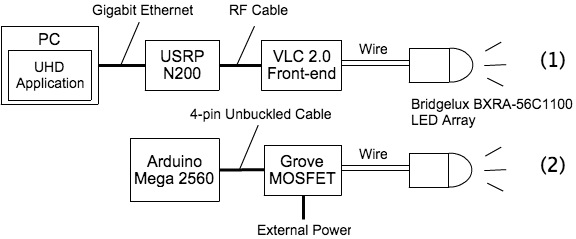
\includegraphics[width=\textwidth]{pic/tx_devices.png} 
      \caption{Transmitter Components} \label{fig:tx_component}
    \end{subfigure}
    \\
    \begin{subfigure}[h]{0.5\textwidth}
      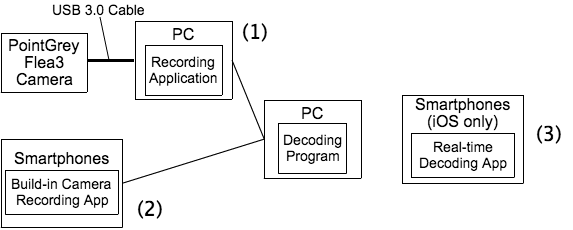
\includegraphics[width=\textwidth]{pic/rx_devices.png} 
      \caption{Receiver Components} \label{fig:rx_component}
    \end{subfigure}
  \caption{System Componenets}
  \label{fig:components}
\end{figure}
%p.11 different frame rate, different device width, different device result
%p.12 tx fps up, distance, exposure
%p.13 iphone/time evaluataion
\section{Evaluation}
\subsection{Experimental Methodology}
 In \autoref{sec:unsync}, we derive the probability of symbol loss and mixed frame. The value is affected by the transmitting frame rate ($T_{f,tx}$), receiving frame rate ($T_{f,rx}$), the read-out time of the camera ($T_r$) and the height of the LED in the received image ($H$). 
 Therefore, we present the experimental results of our unsynchronized VLC system with respect to these factors. The performance metrics we use in the experiments are Packet Reception Rate (PRR) and throughput.

 Each symbol represents 4-bit, and thus we have 16 symbols. 
 The symbol-to-frequency mapping table is generated by.... (formula).
 \autoref{fig:exp1_setup} shows a photo illustrating our setup. 

\subsection{Different Receiving Frame Rate}
First, we want to show the improvement of the decoding performance due to the design of the symbol delimiter, the sequence number, and the parity symbol. 

We alter the receiving frame rate to obtain different tx/rx frame rate ratios from 0.9 to 2 to force unsynchronized transmitter and receiver pairs. That is, we fix the transmitting frame rate at 30 fps, and alter the receiving frame rate from 15 fps to 33 fps. We randomly generate 20 string sequences for each of the three settings: (1) no additional schemes; (2) with only symbol delimiter; and (3) with symbol delimiter, sequence number,  and parity symbol. 
The length of the string sequence is 20 bytes. Note that we also record the videos at random starting time to introduce random phase difference between the transmitter and the receiver.

\autoref{fig:exp1_1} shows the result. When the receiving frame rate and the transmitting frame rate are very close to each other, the first setting has slightly lower PRR, as a number of received image frame will be mixed with two symbols and a portion of them will be demodulated correctly. The other two settings perform similarly. 
However, as the difference between the frame rates increase, the differences in PRRs become very obvious. 

% \begin{figure}[!htb]
%   \centering
%   %\hspace{-5em}
%   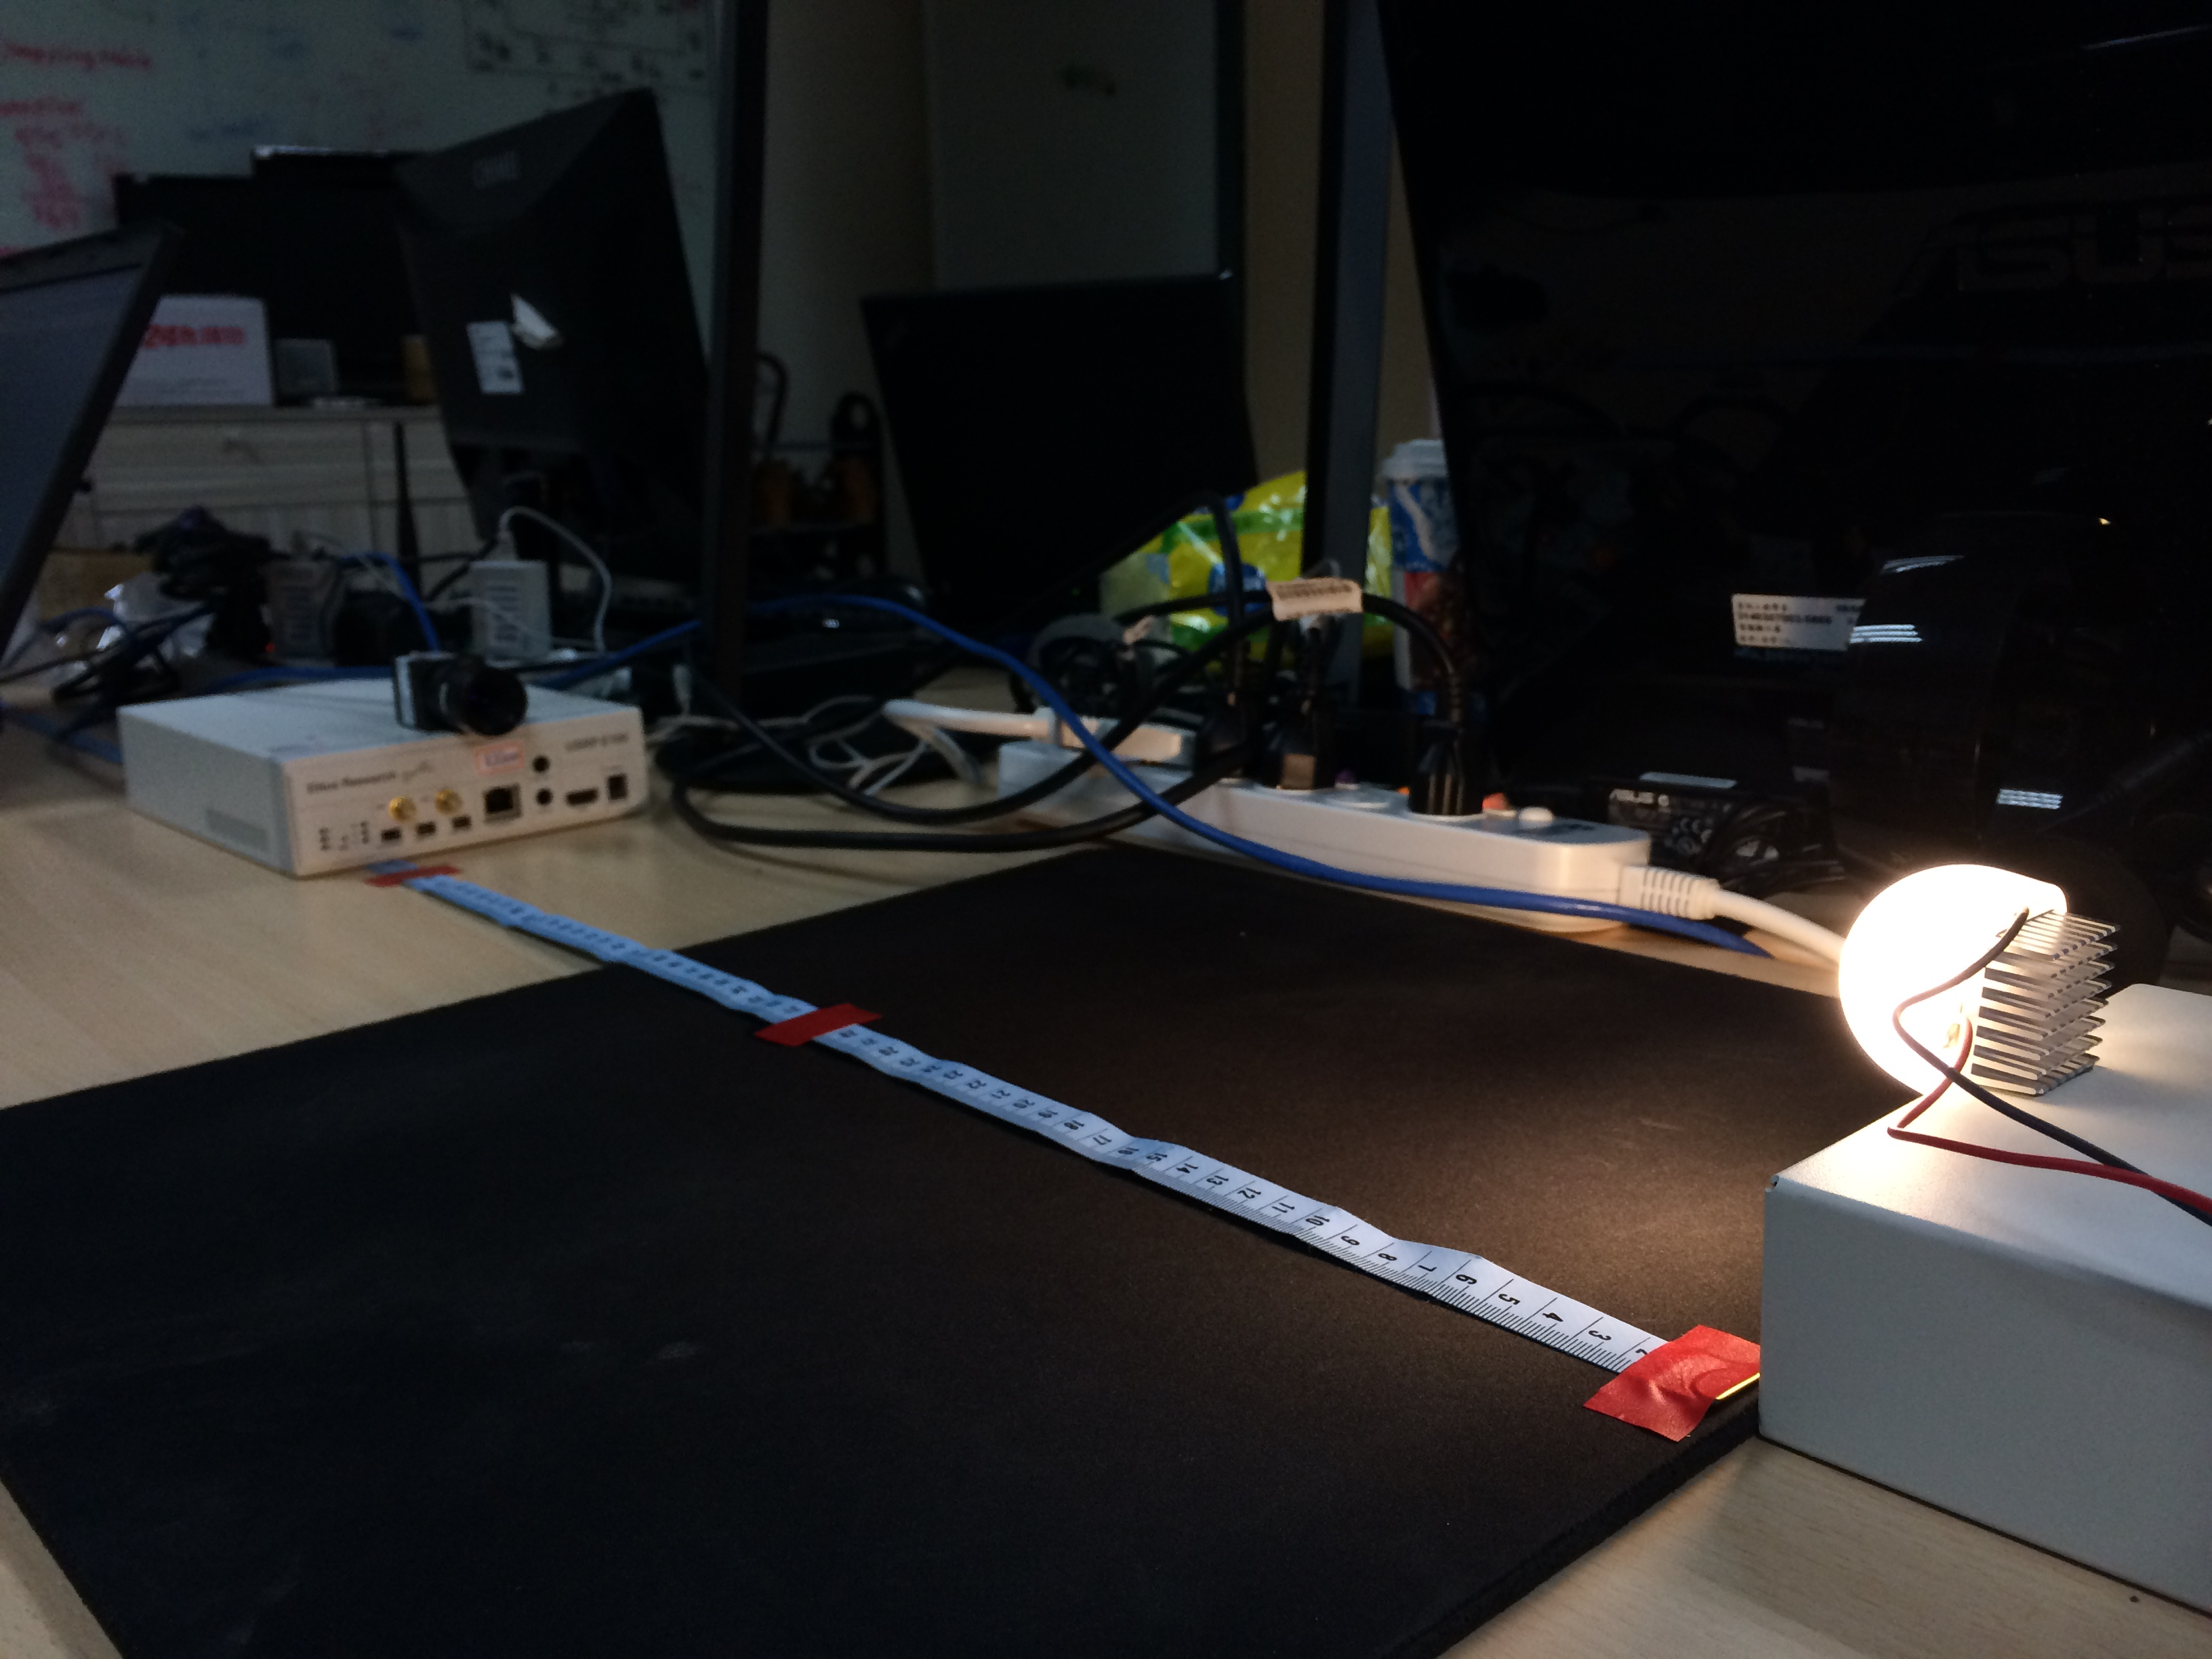
\includegraphics[scale=0.075]{fig/exp4_setup.JPG}
%   \caption{Experimental setup photo.}
%   \label{fig:exp1_setup}
% \end{figure}
\begin{figure}[!t]
\centering
  \begin{subfigure}[h]{0.2\textwidth}
  \includegraphics[width=\textwidth]{pic/env_smartphone.JPG}
  \caption{}
  \end{subfigure}
  ~ 
  \begin{subfigure}[h]{0.2\textwidth}
  \includegraphics[width=\textwidth]{pic/env_flea.JPG}
  \caption{}
  \end{subfigure}
\caption{Experimental setup photos with different Receivers: (a) Smartphone (b) Flea3}
\label{fig:exp1_setup}
\end{figure}

The $P_{miss}^ \prime$ and parity symbol ratio are also shown in \autoref{fig:exp1_1}. 
For the third setting, we use $P_{miss}$ to determine the number of parity symbols required to be inserted into a packet. When the receiving frame rate is higher than 19.5 fps, the parity symbol ratio is configured to be 0.25, which means for every three symbols, we add a parity symbol. (It is possible to use a parity symbol rate less than 0.25, following the pink line in the figure. However, we do not discuss such a case here, and will discuss the maximum throughput in \autoref{sec:maxthroughput}.) When the receiving frame rate is between 19.5 and 18 fps, we use a parity symbol ratio of 0.33. When the receiving frame rate is lower than 18 fps, we use a parity symbol ratio of 0.5, which means for every symbol, we transmit twice.
With all 3 schemes, close to 100\% of the packets are received correctly, while the other two settings rapidly lose the ability to receive correct packets when the difference between frame rates increases. The results verify that our design can indeed address the issues caused by unsynchronized transmitter and receiver pair. 

We can see when the receiving frame rate and the transmission frame rate are close, the setting with the symbol delimiter has the highest throughput. As the difference between the frame rates increases, the throughput of the third setting decreases due to the large parity symbol ratio.

\subsection{Varying Inter-frame Interval}
% \begin{figure}[!htb]
%   \centering
%   %\hspace{-2em}
%   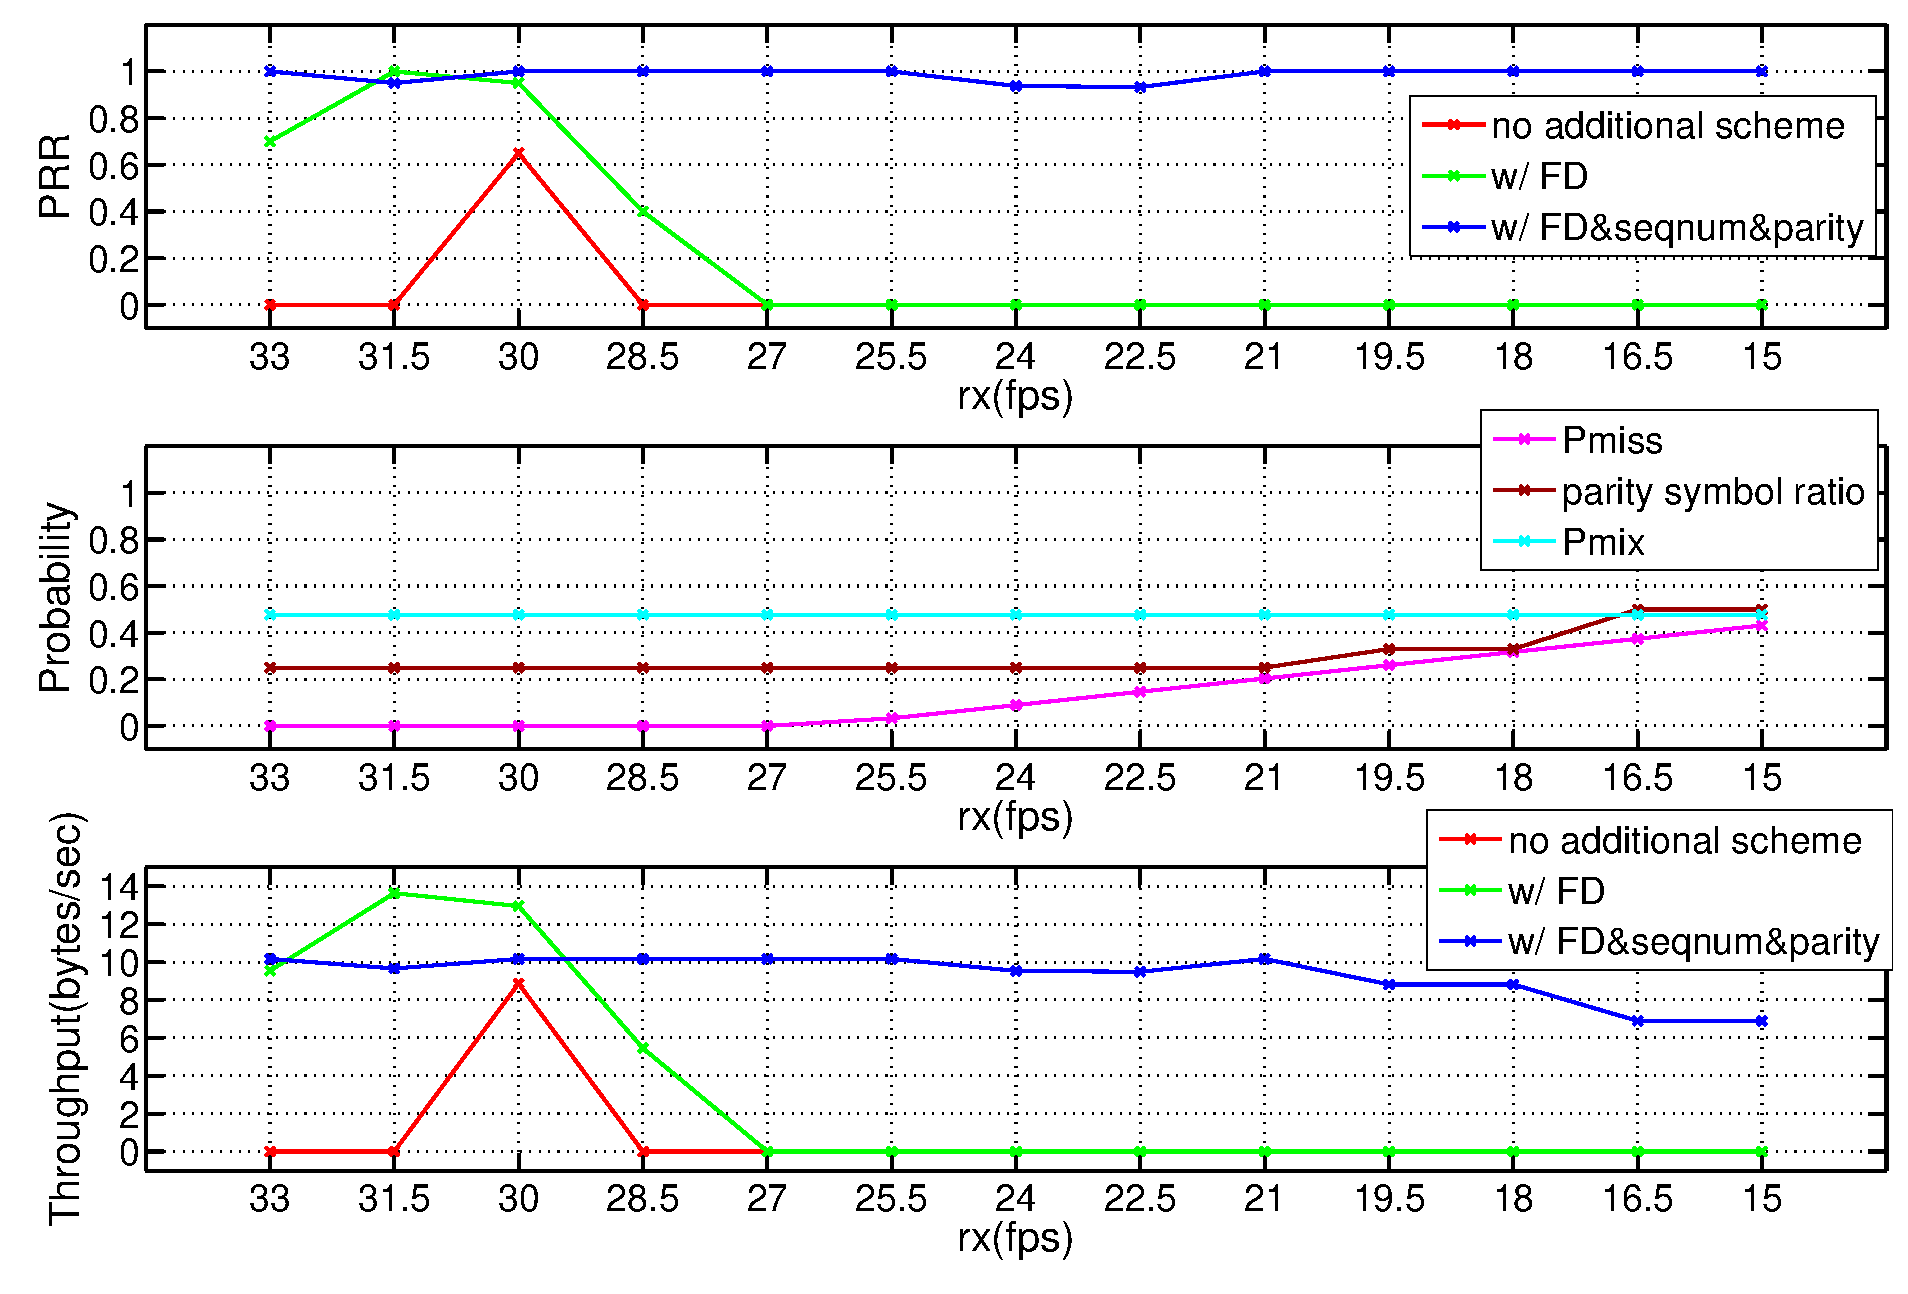
\includegraphics[scale=0.25]{fig/exp1_new.eps}
%   \caption{Result under different rx fps.}
%   \label{fig:exp1_1}
% \end{figure}
% \begin{figure}[!htb]
%  % \centering
%   \hspace{-5em}
%   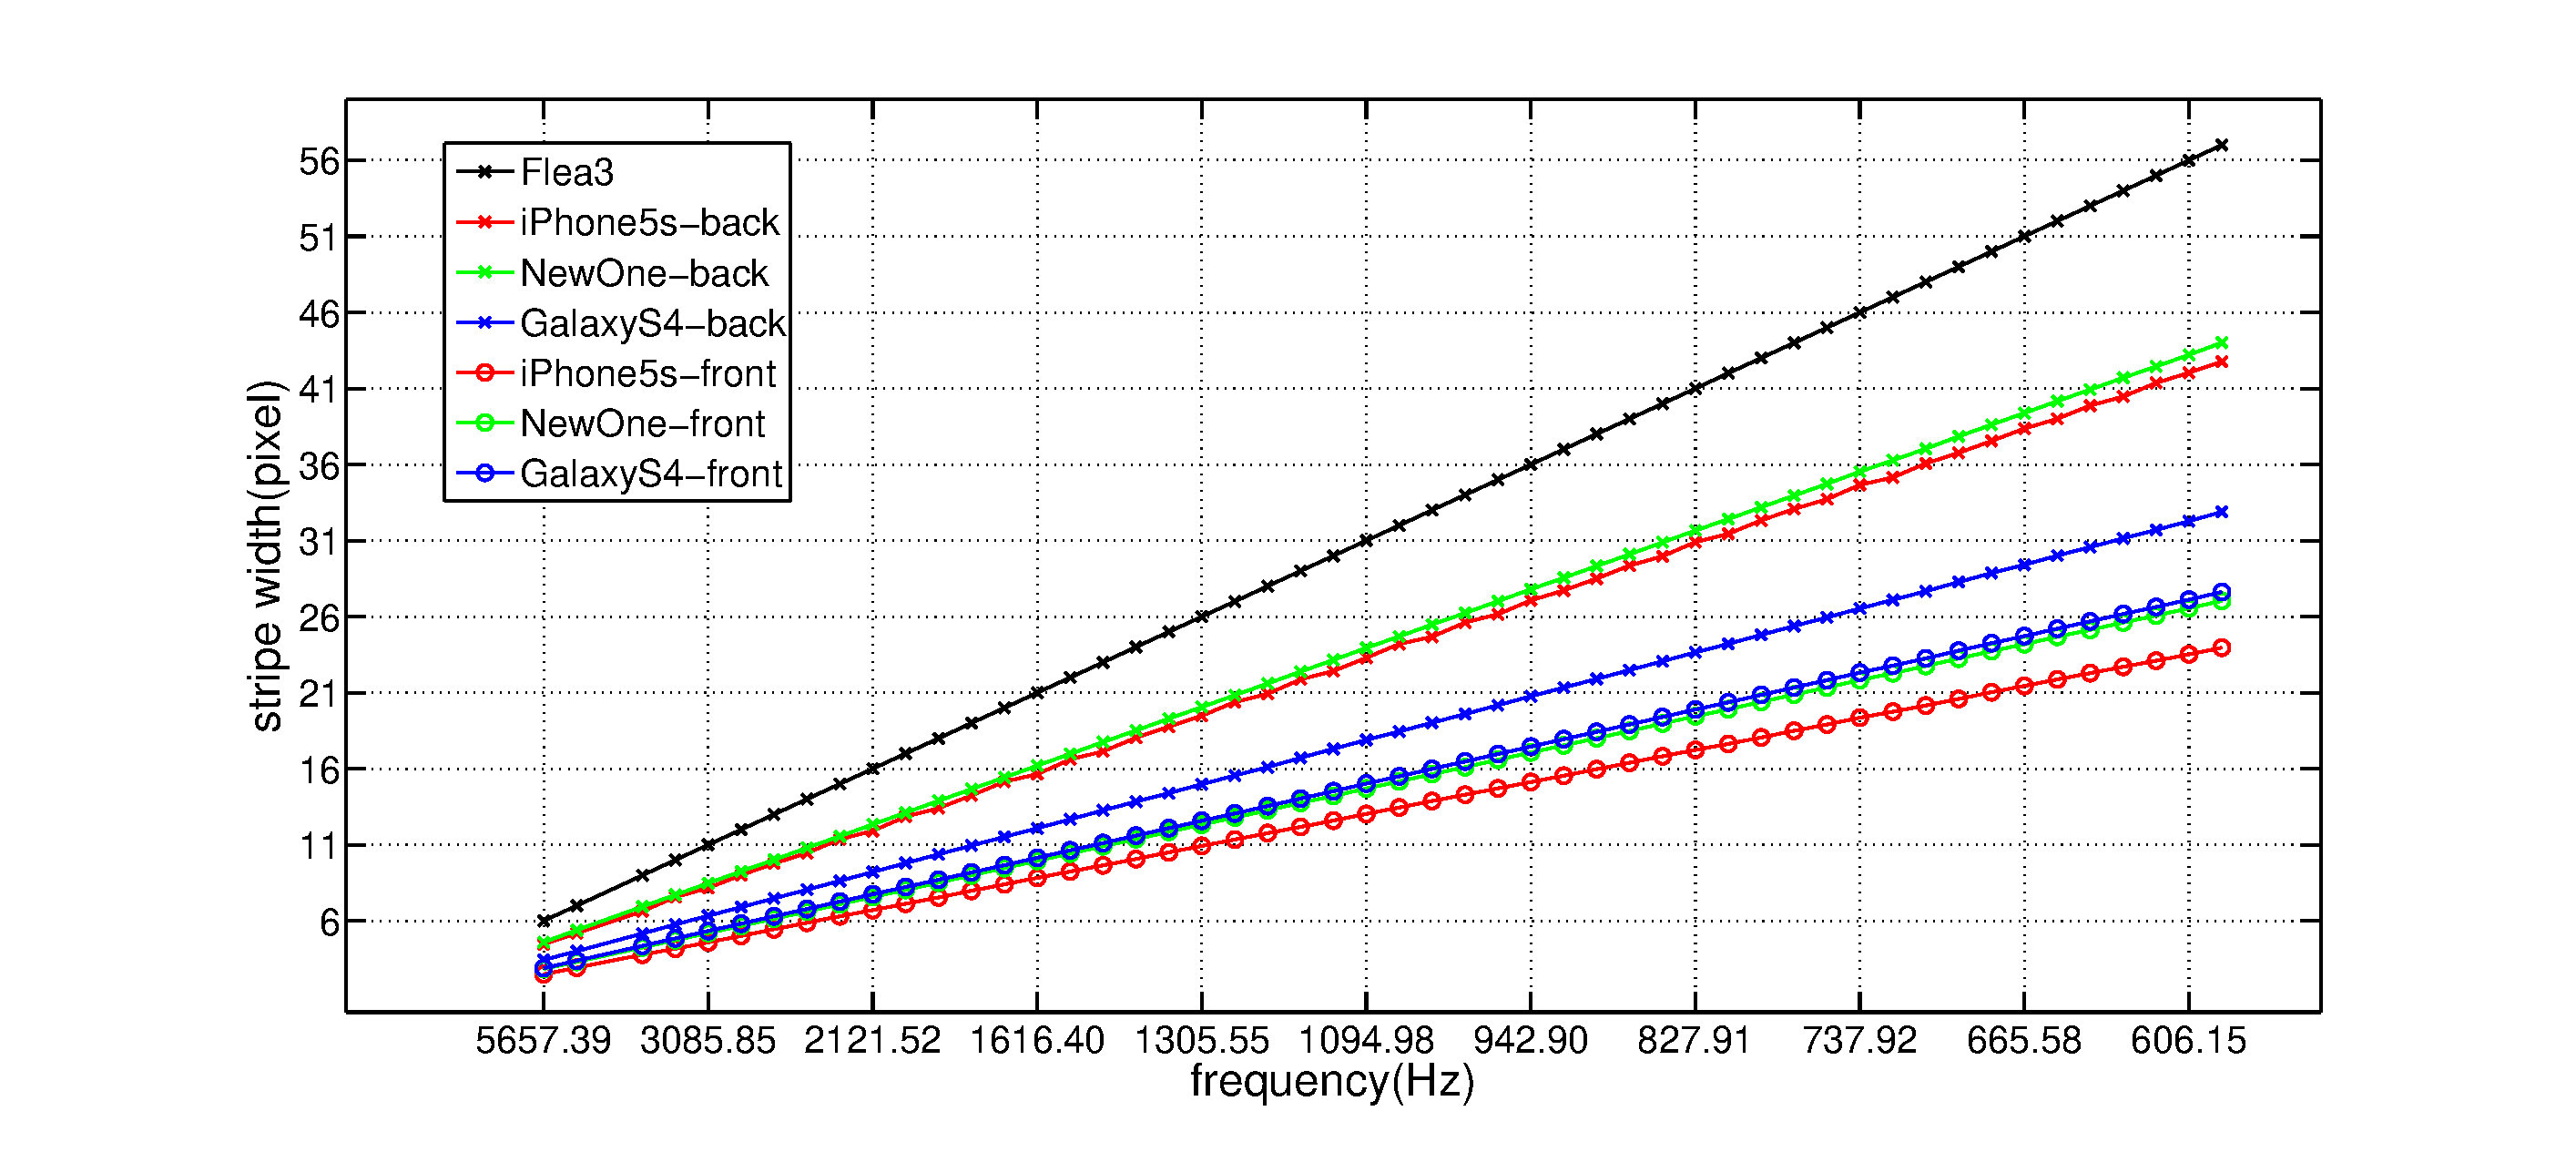
\includegraphics[scale=0.2]{fig/exp2_tr_new.eps}
%   \caption{Pixel width under different smartphone devices.}
%   \label{fig:exp2_tr}
% \end{figure}
% \begin{figure}[!htb]
%  % \centering
%   \hspace{-3em}
%   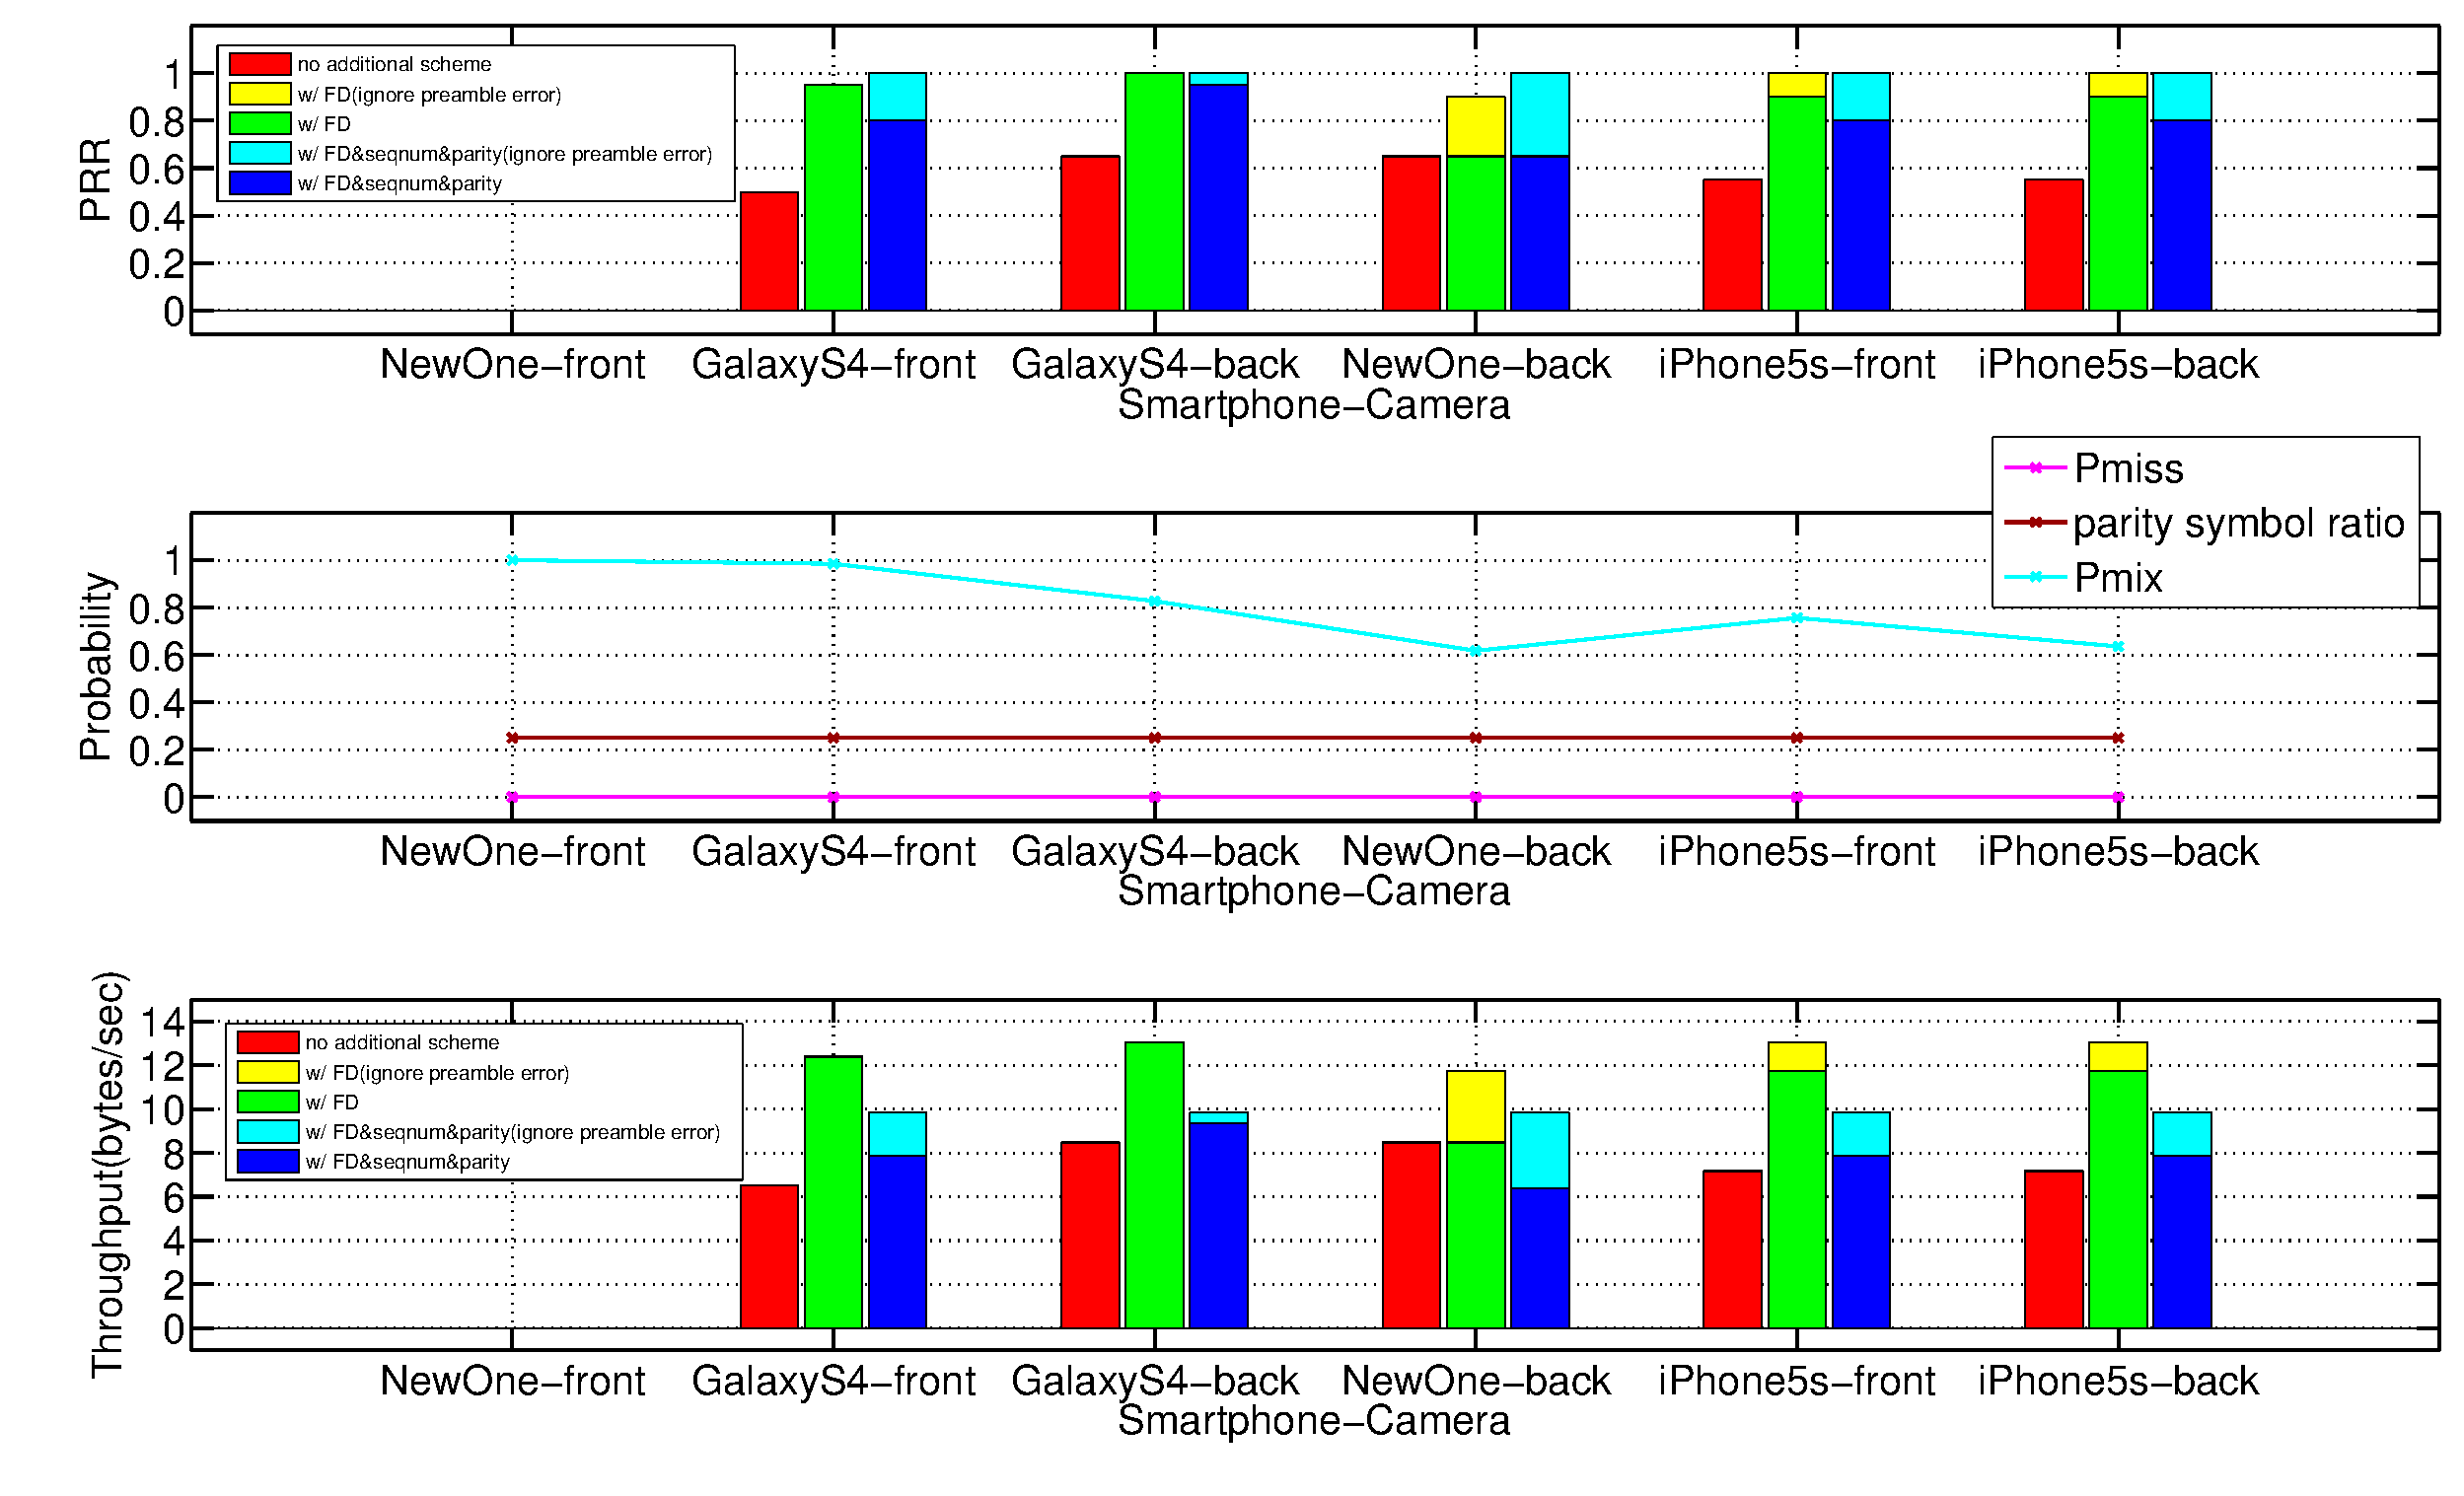
\includegraphics[scale=0.2]{fig/exp2_refine.eps}
%   \caption{Result under different smartphone devices.}
%   \label{fig:exp2_1}
% \end{figure}

\begin{figure*}[!t]
  %\centering
	\begin{subfigure}[h]{0.3\textwidth}
	  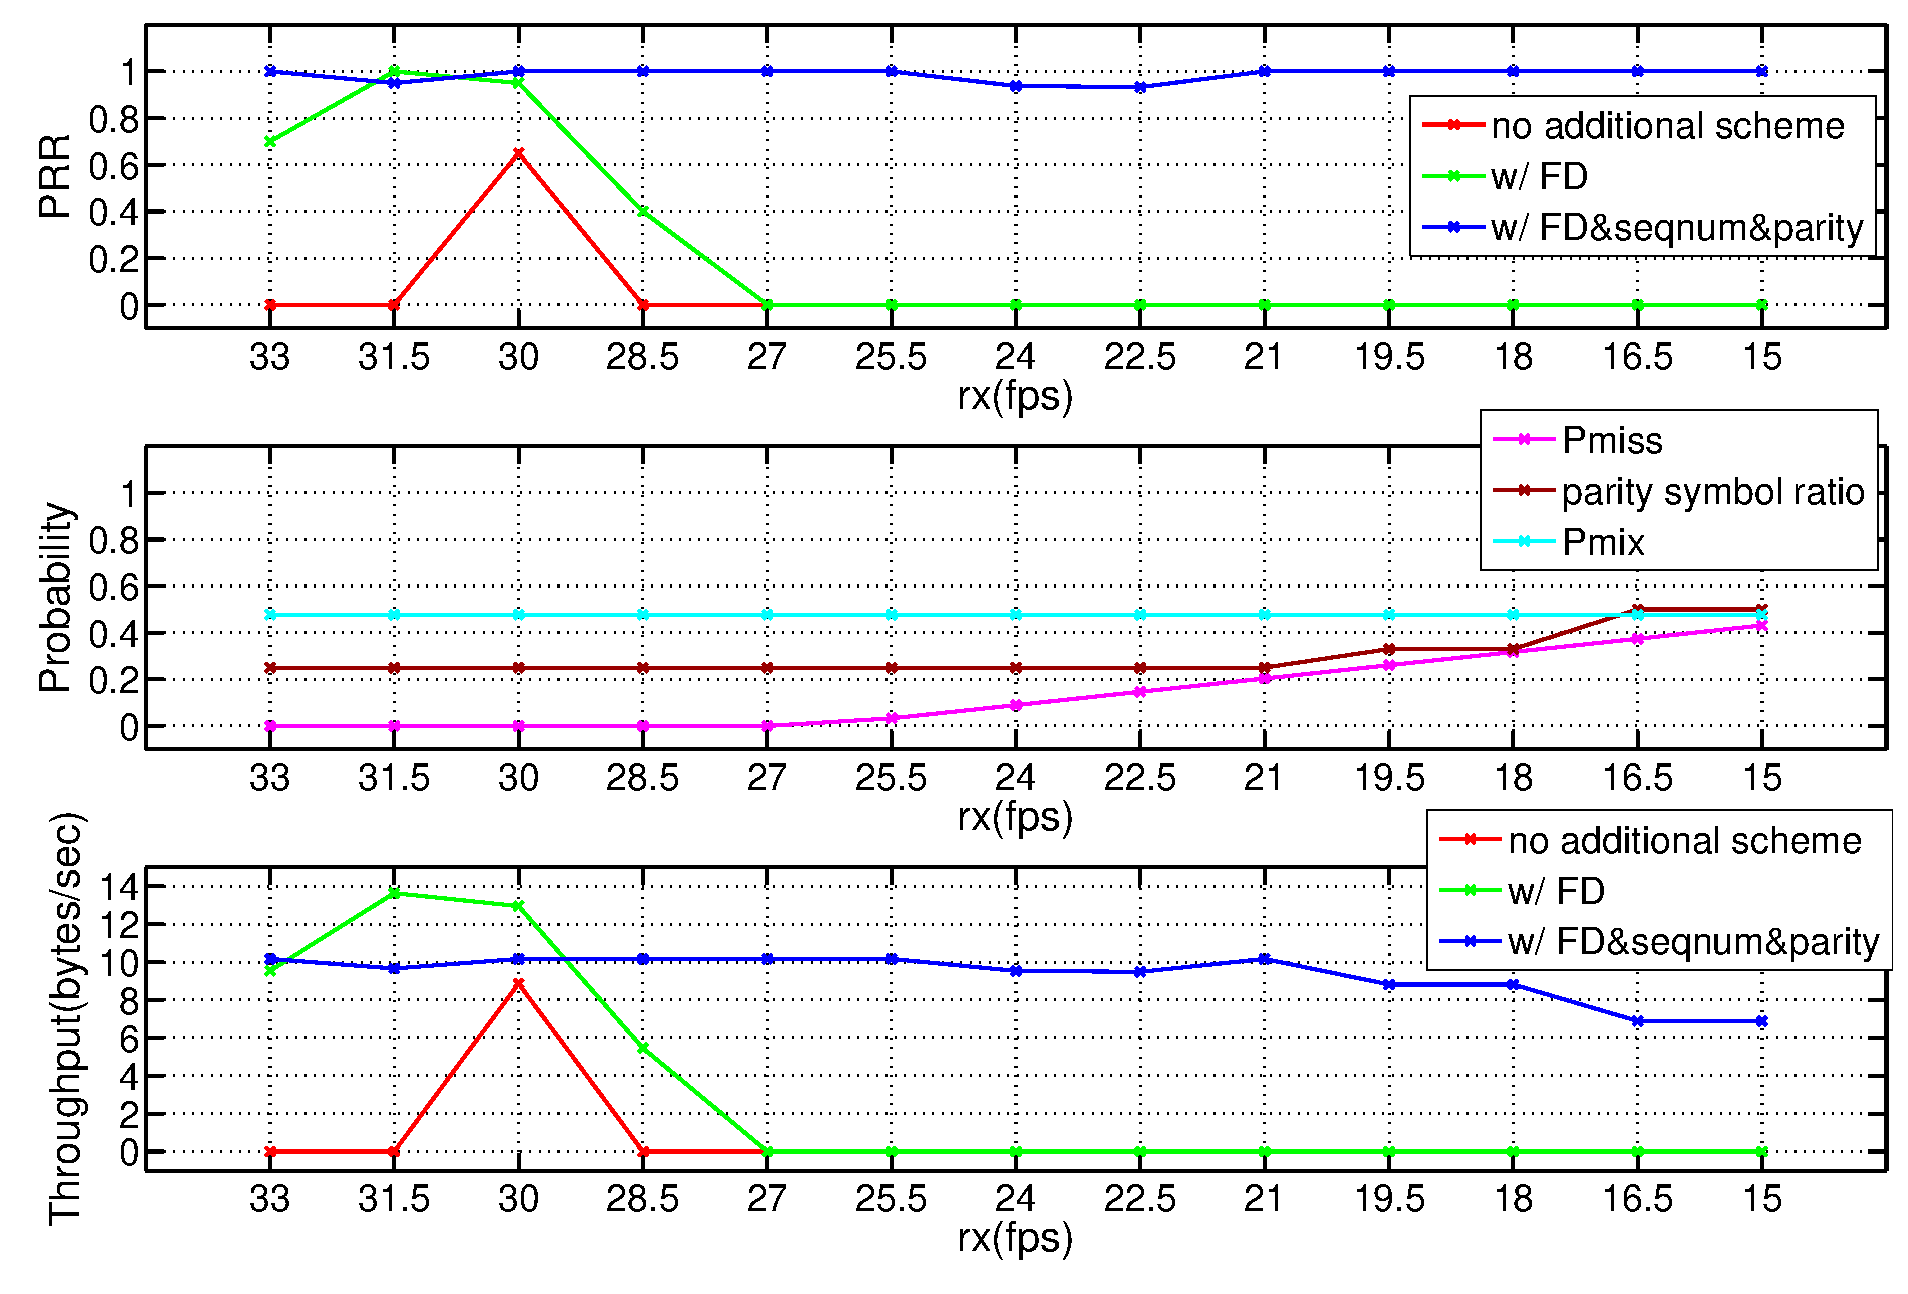
\includegraphics[width=\textwidth]{fig/exp1_new.eps}
	  \caption{}
	  \label{fig:exp1_1}
	\end{subfigure}
	~
	\begin{subfigure}[h]{0.35\textwidth}
	  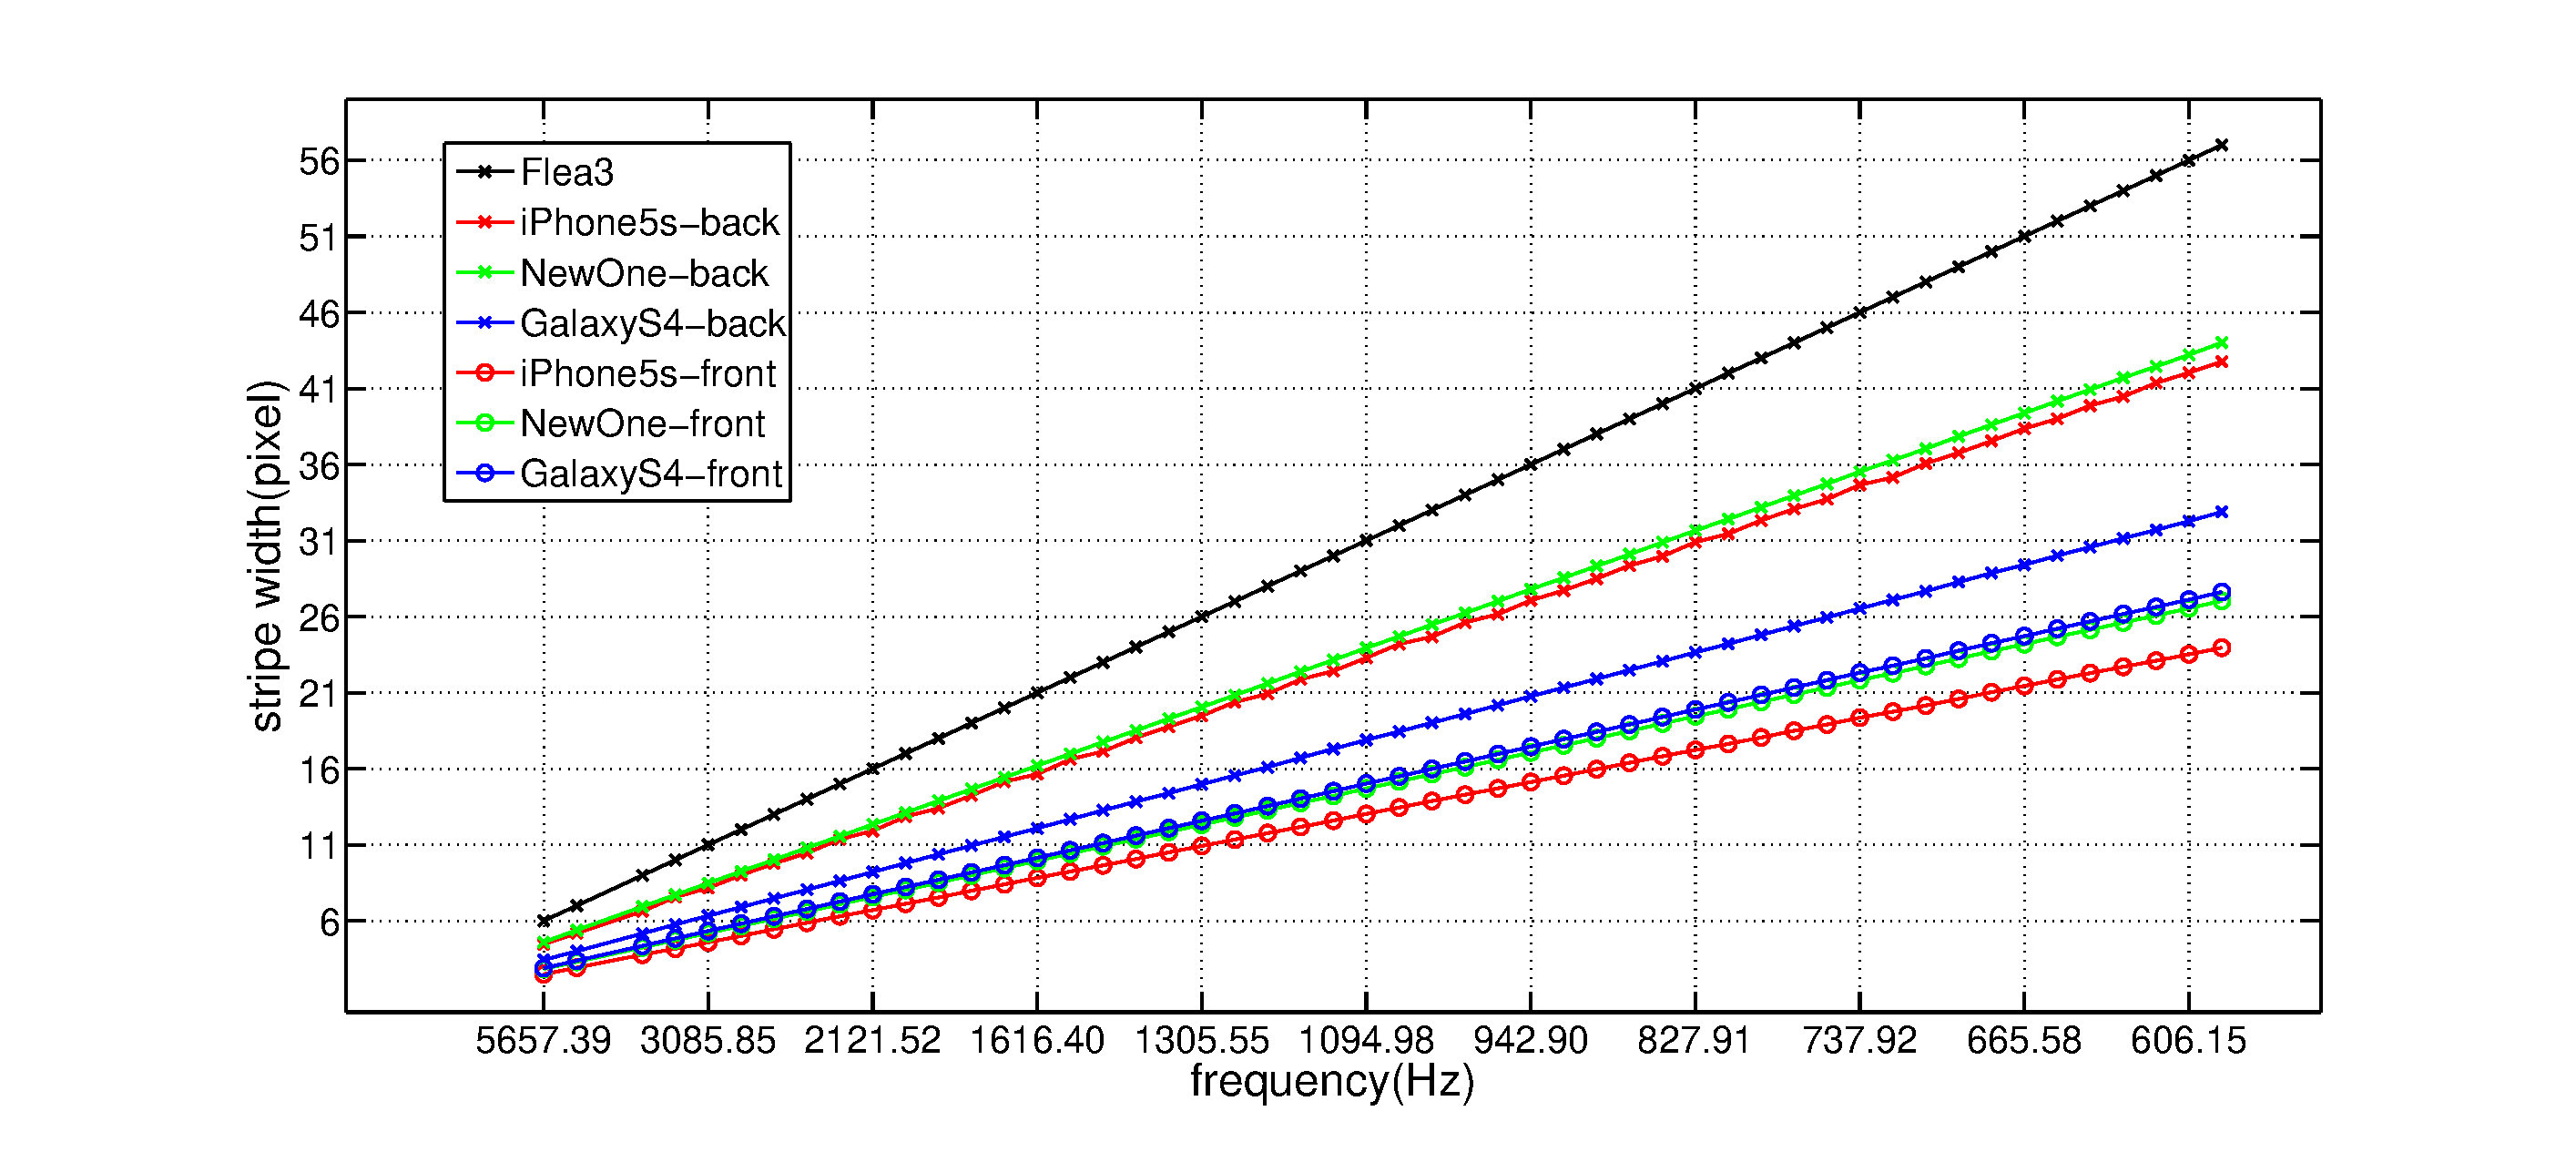
\includegraphics[width=\textwidth]{fig/exp2_tr_new.eps}
	  \caption{}
  	  \label{fig:exp2_tr}
	\end{subfigure}
	~
	\begin{subfigure}[h]{0.3\textwidth}
  	  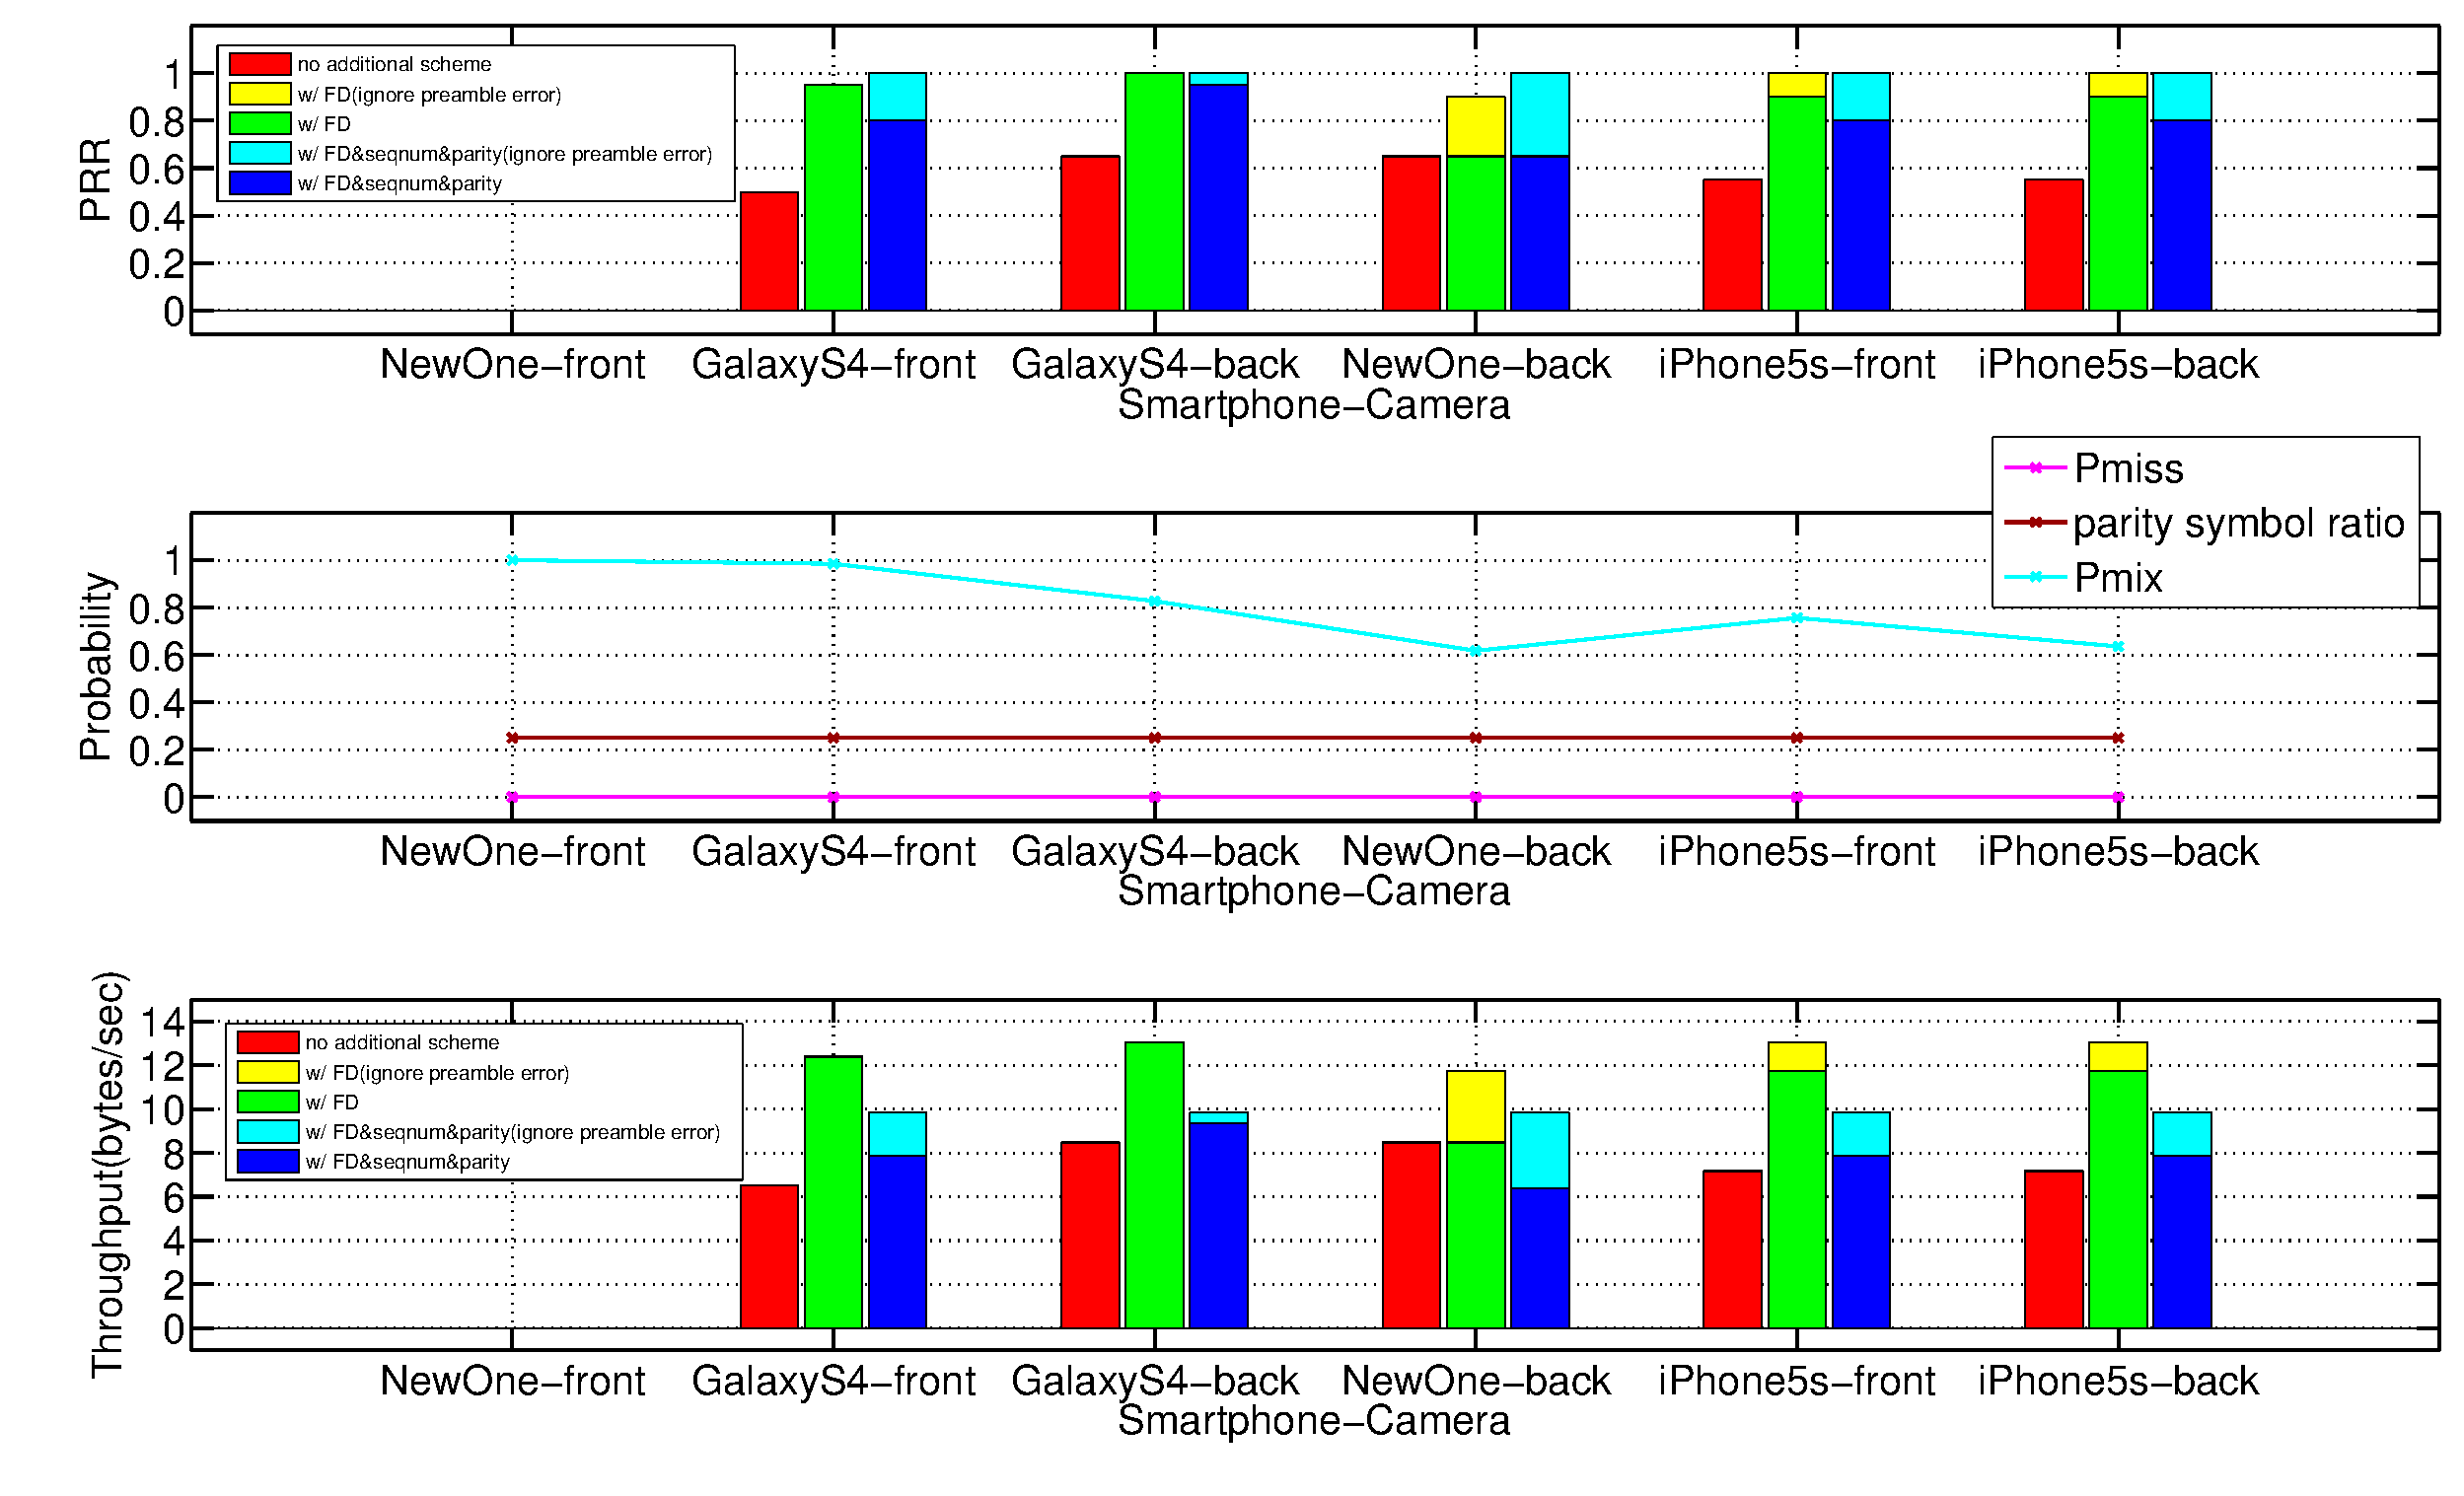
\includegraphics[width=\textwidth]{fig/exp2_refine.eps}
      \caption{}
      \label{fig:exp2_1}
    \end{subfigure}
    \caption{(a) Result under different rx fps. (b) Pixel width under different smartphone devices. (c) Result under different smartphone devices.}
    \label{}
\end{figure*}
According to~\cite{hu2013lightsync}, the receiving frame rate of smartphone cameras exhibit more variability for several reasons. Even when the average frame rate appears steady, the inter-frame interval still varies. 
In order to show the improvement with our new design scheme, we emulate this phenomena with a system with time varying inter-frame interval. 
However, it is hard to alter the receiving frame rate while receiving frames. We therefore use the Flea3 camera with fixed receiving frame rate and alter the transmitting frame rate before transmitting every symbol. 

To simulate the various of transmitting frame rate, we use a truncated normal distribution with the mean value of 36.9458 fps, the standard deviation of 3.94, the min value 31.03 fps and the max value 42.86 fps. The values are based on observations presented in~\cite{hu2013lightsync}, which states that the receiving frame rate fluctuates significantly between 21 to 29 fps for an entirely white foreground, with an average of around 25 fps. 

We again generate 20 random string sequences. The length of each string sequence is 20 bytes. For each transmitting symbol, we randomly pick a number from the truncated normal distribution and transmit the symbol with the generated frame rate.
We use the PointGrey Flea3 camera to record the video at fixed 30 fps. 

% \autoref{tab:norm_result} shows the result of PRR and throughput.
% First, we want to know how frequently mixed frame or lost symbol occur. Thus, we use the average transmitting frame rate 36.9458 fps to calculate the probability. We get $P_{miss}$ = 0.0501 and $P_{mix}$ = 0.5877.
% We can see that with no additional schemes, the PRR is 0 since there are a large number of mixed frames. With only the symbol delimiter setting, the PRR is still 0 because there is a non-zero probability to have missed symbol. With all three schemes, the PRR is 1. It is worth mentioning that we use a lower parity symbol ratio to increase the throughput in this experiment.

% \begin{table}[!htb]
% \centering
% \caption{PRR and Throughput under various inter-frame interval.}
%         %\tabcolsep=1cm
%         %\tabcolsep=0.08cm
%         \begin{tabular}{lcc}
%         \hline Setting & PRR & Throughput\\ 
%         \hline \hline
%         No additional schemes & 0 & 0 bytes per second\\
%         With only symbol delimiter   & 0 & 0 bytes per second \\
%         With symbol delimiter, sequence number and parity symbol ratio 0.125 & 1 & 13.94 bytes per second\\
%         With symbol delimiter, sequence number and parity symbol ratio 0.143 & 1 & 13.68 bytes per second\\
%         With symbol delimiter, sequence number and parity symbol ratio 0.167 & 0.95 & 11.89 bytes per second\\
%         With symbol delimiter, sequence number and parity symbol ratio 0.2 & 1 & 12.31 bytes per second\\
%         %With frame delimiter, sequence number and parity symbol ratio 0.25 & 1 & 12.1134\\
%         %With frame delimiter, sequence number and parity symbol ratio 0.33 & 1 & 10.8664 \\
%         %With frame delimiter, sequence number and parity symbol ratio 0.5 & 1 & 8.4933 \\
%         \hline
%         \end{tabular}
%         \label{tab:norm_result}
% \end{table}

\subsection{Different Smartphone Cameras}
Third, we use several smartphones to compare the decoding performance under the three previous mentioned settings. 
Note that the receiving frame rate of the smartphones are not fixed. Moreover, the read-out time and the resolution of the camera of smartphones are also different. These will affect the probabilities of symbol loss and mixed frame. We again generate 20 random string sequences. The length of each string sequence is 20 bytes. 

As the read-out time of the smartphones are not the same. This means different smartphone cameras may observe the different pixel width (signal period) under the same transmitting frequency. Therefore we use the preamble symbol to calibrate the $T_r$ to minimize the error of the period estimates of all subsequent symbols in the packet. \autoref{fig:exp2_tr} shows the pixel width of different smartphone cameras. %We use the pixel width of Flea3 as the base (the X-axis), and the Y-axis represents the observed pixel width. Generally, the pixel width grows linearly. What we need to do is to calibrate the lines to fit the top black line. 

\autoref{fig:exp2_1} shows the result. The X-axis shows different smartphone cameras. We first calculate $P_{miss}$ by averaging the frame rate of each smartphone camera. The obtained values are all zeros since the average fps are close to 30. However, we can see that $P_{mix}$ is high.

For the first setting, we can see the PRR is about 50\% to 60\%. The result also shows that when the $P_{mix}$ is higher, PRR of the first setting gets lower.
For the second and third settings, basically that PRRs are similar since no symbol miss take place. However, we can see that most of the devices show that the third setting gets lower PRR then the second setting. Some of the devices also show that the third setting gets lower PRR then the first setting. Furthermore, the overall PRR is on the low side. We think the problem is due to decoding error. Because of the instability of the smartphone cameras, if the received pixel width of the preamble has slightly error, it will affect the third setting very much because the pixel width range we use in the third setting is larger than the first two settings. The yellow and cyan bars in the figure represent the result ignoring the preamble error. We can see that PRRs of the second and third settings are very close to 1. (From this experiment, we can see that the second setting is good enough for the communications in spite of using different smartphones. However, the current setting uses regular video recording mode rather than preview mode, and the receiver is very close to the transmitter. That is, the are many factors not considered yet and these will be discussed in the following subsection.) Therefore, the error are mainly caused by the preamble calibration rather than the unsynchronized issues. To address the preamble calibration error, we can transmit more preamble symbols at the beginning of the packet and average them when receiving these symbols. This solution can minimize the error caused by calibration but will increase the packet overhead at the same time.

We also found that the front-facing camera of HTC NewOne cannot decode any packet in all three settings. We observed that the behavior of the camera records every frame twice. Even when we extract half of the frames in the video, it is still not able to decode.
Therefore, we think the problem is not related to our decoding method.
Our results indicate that, the second setting can obtain the maximum throughput in most settings.

% \begin{figure}[!t] 
%  %\centering
%   \hspace{-2em}
%   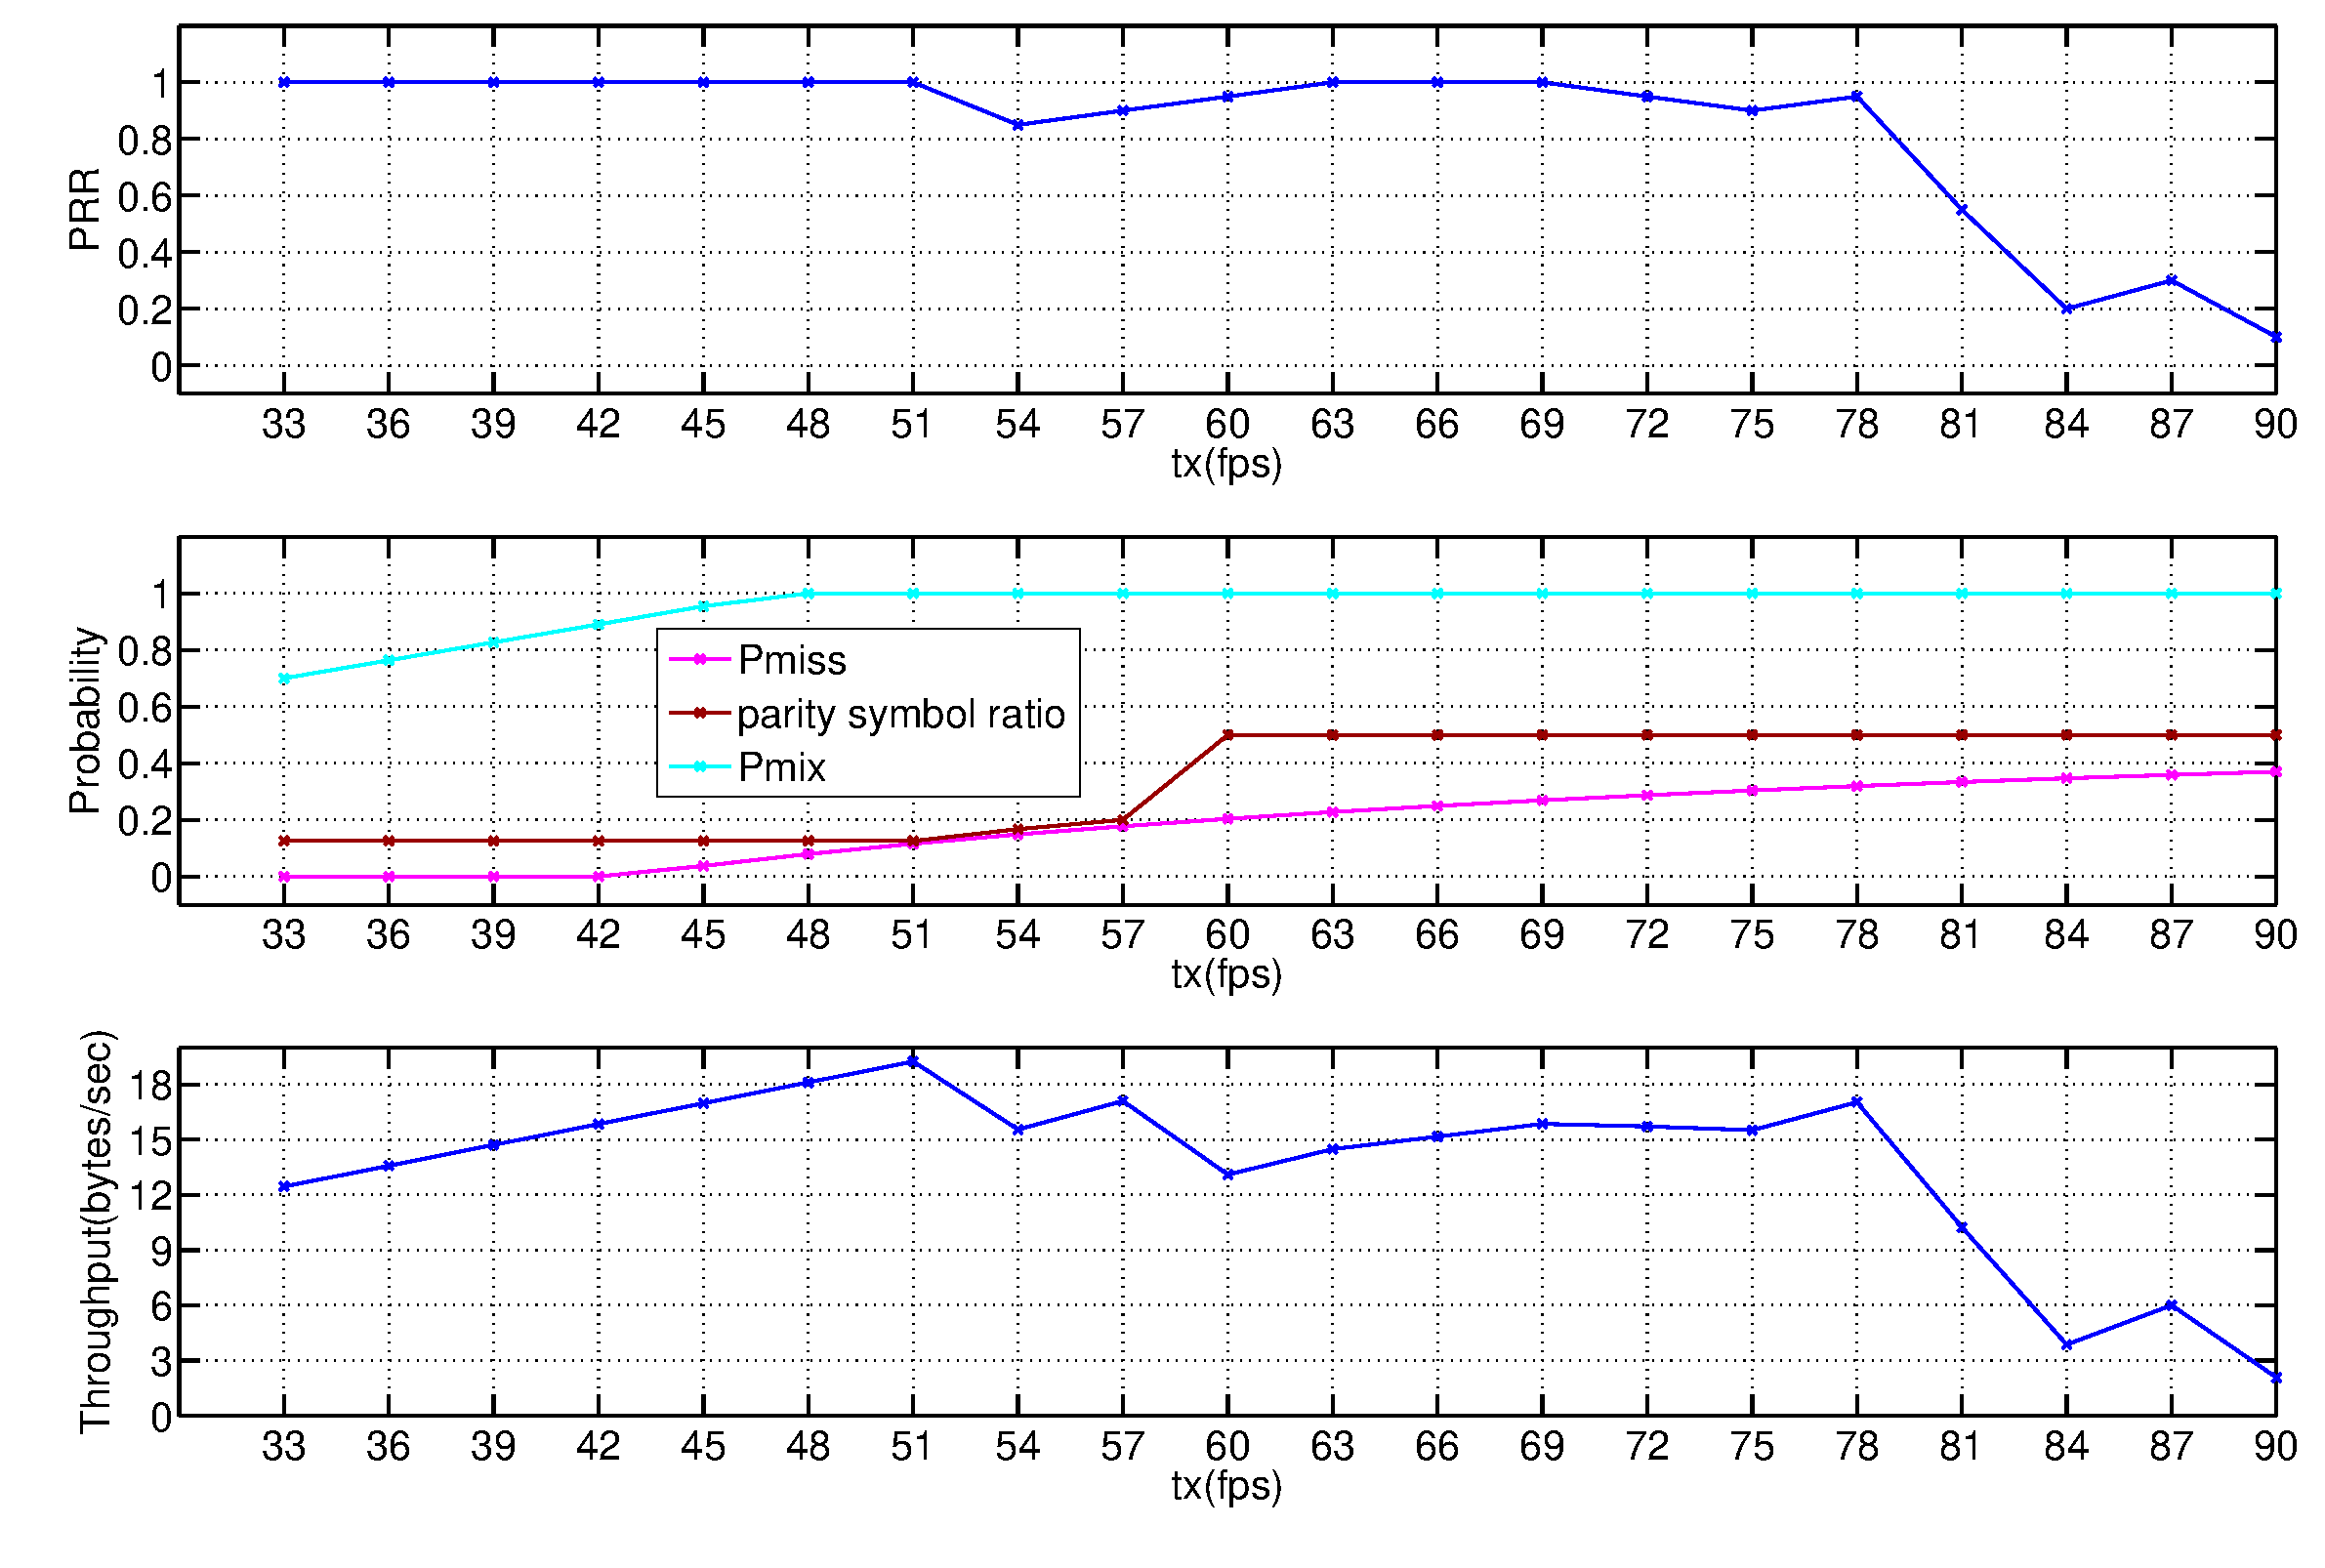
\includegraphics[scale=0.2]{fig/exp3_iphone5s_new_modify.eps}
%   \caption{Result of iPhone5s under different transmitting frame rate.}
%   \label{fig:exp3_3}
% \end{figure}
% \begin{figure}[!htb] 
%  %\centering
%   %\hspace{-3em}
%   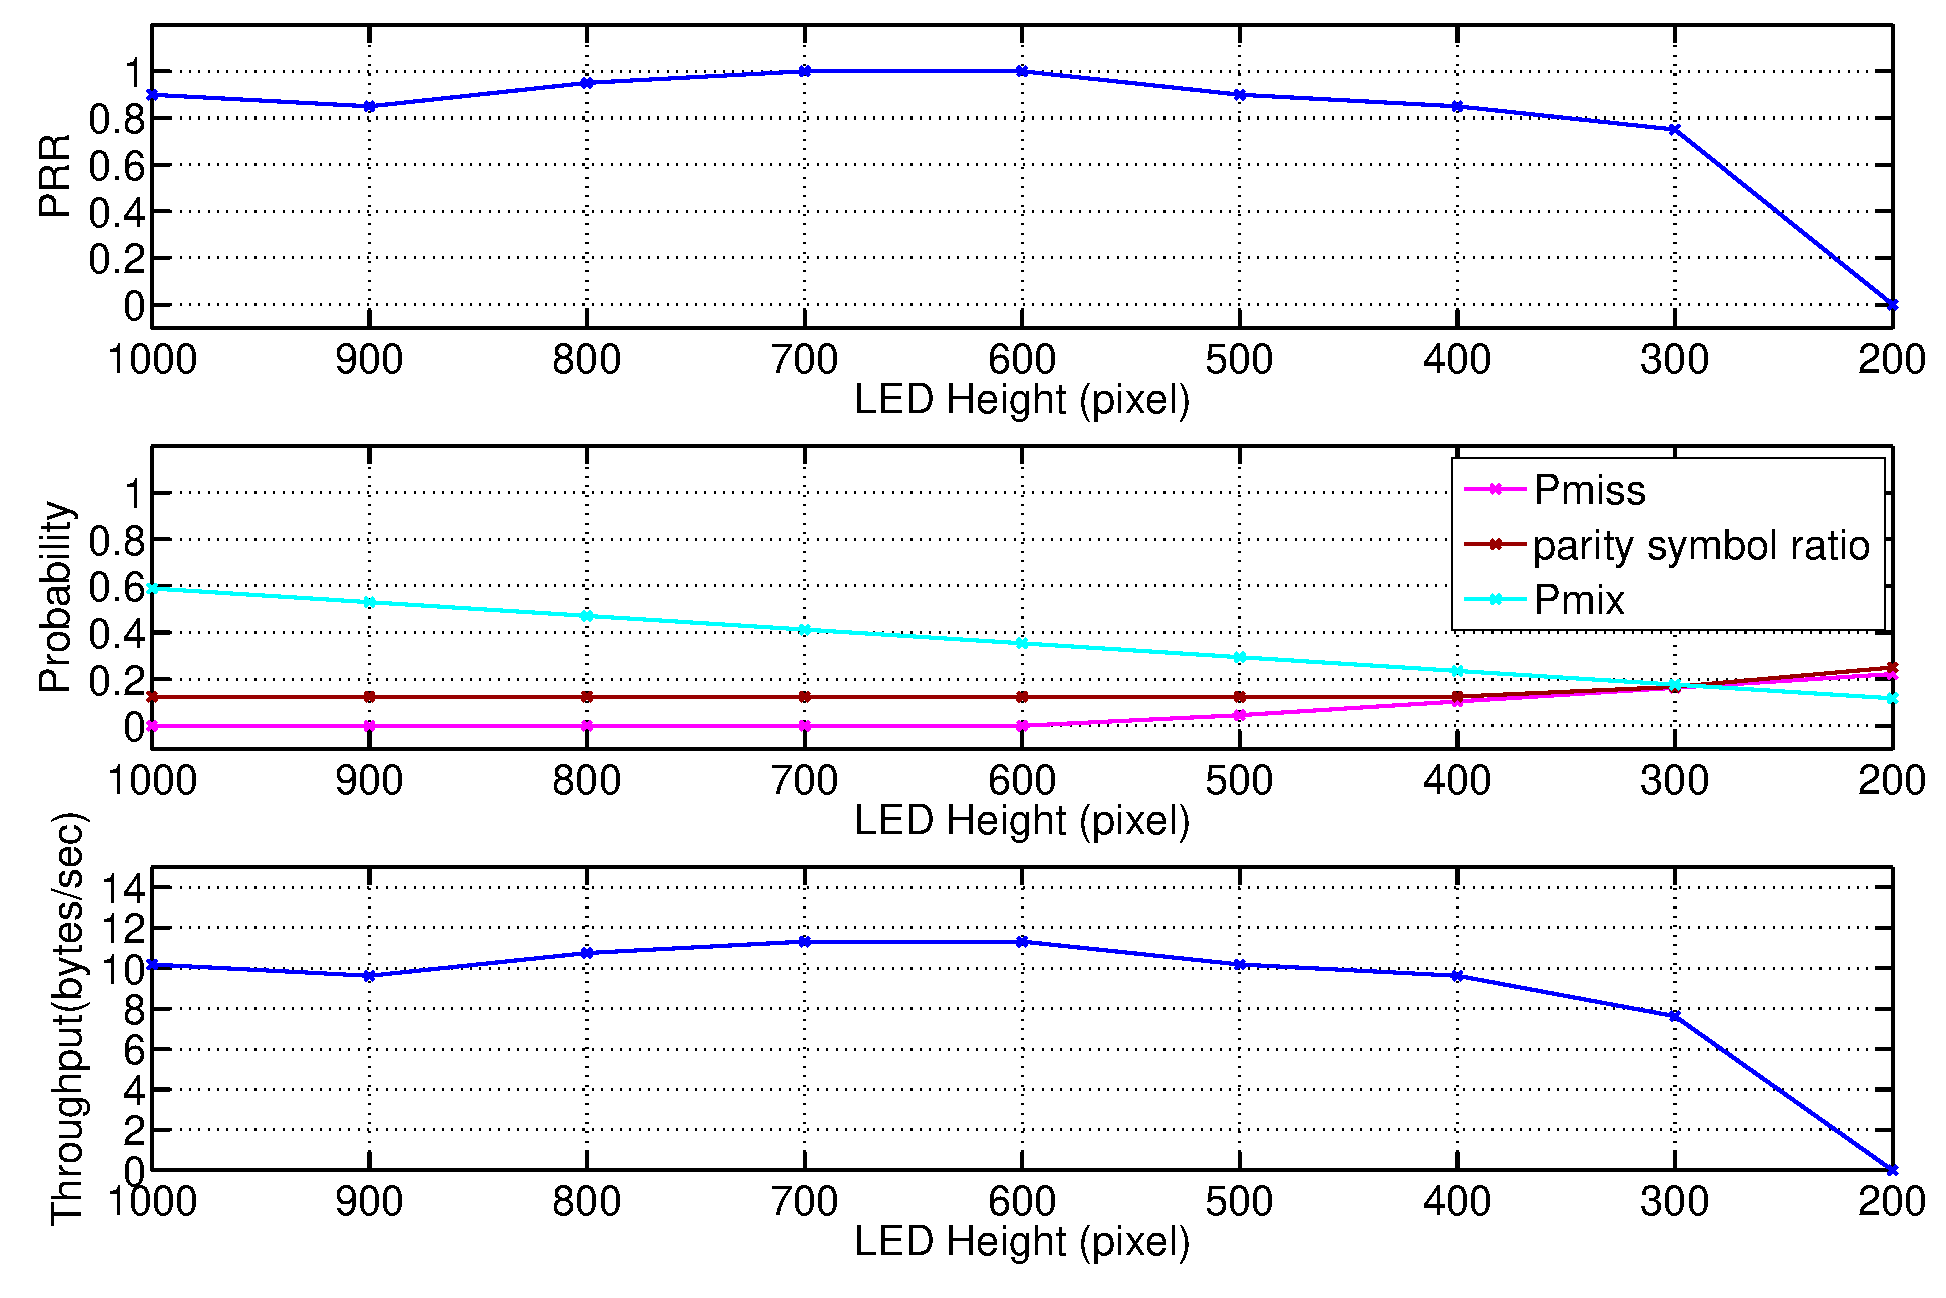
\includegraphics[scale=0.25]{fig/exp4_iphone5s_new.eps}
%   \caption{Result of iPhone5s under different LED height.}
%   \label{fig:exp4_2}
% \end{figure}
\begin{figure*}[!t]
  %\centering
	\begin{subfigure}[h]{0.3\textwidth}
	  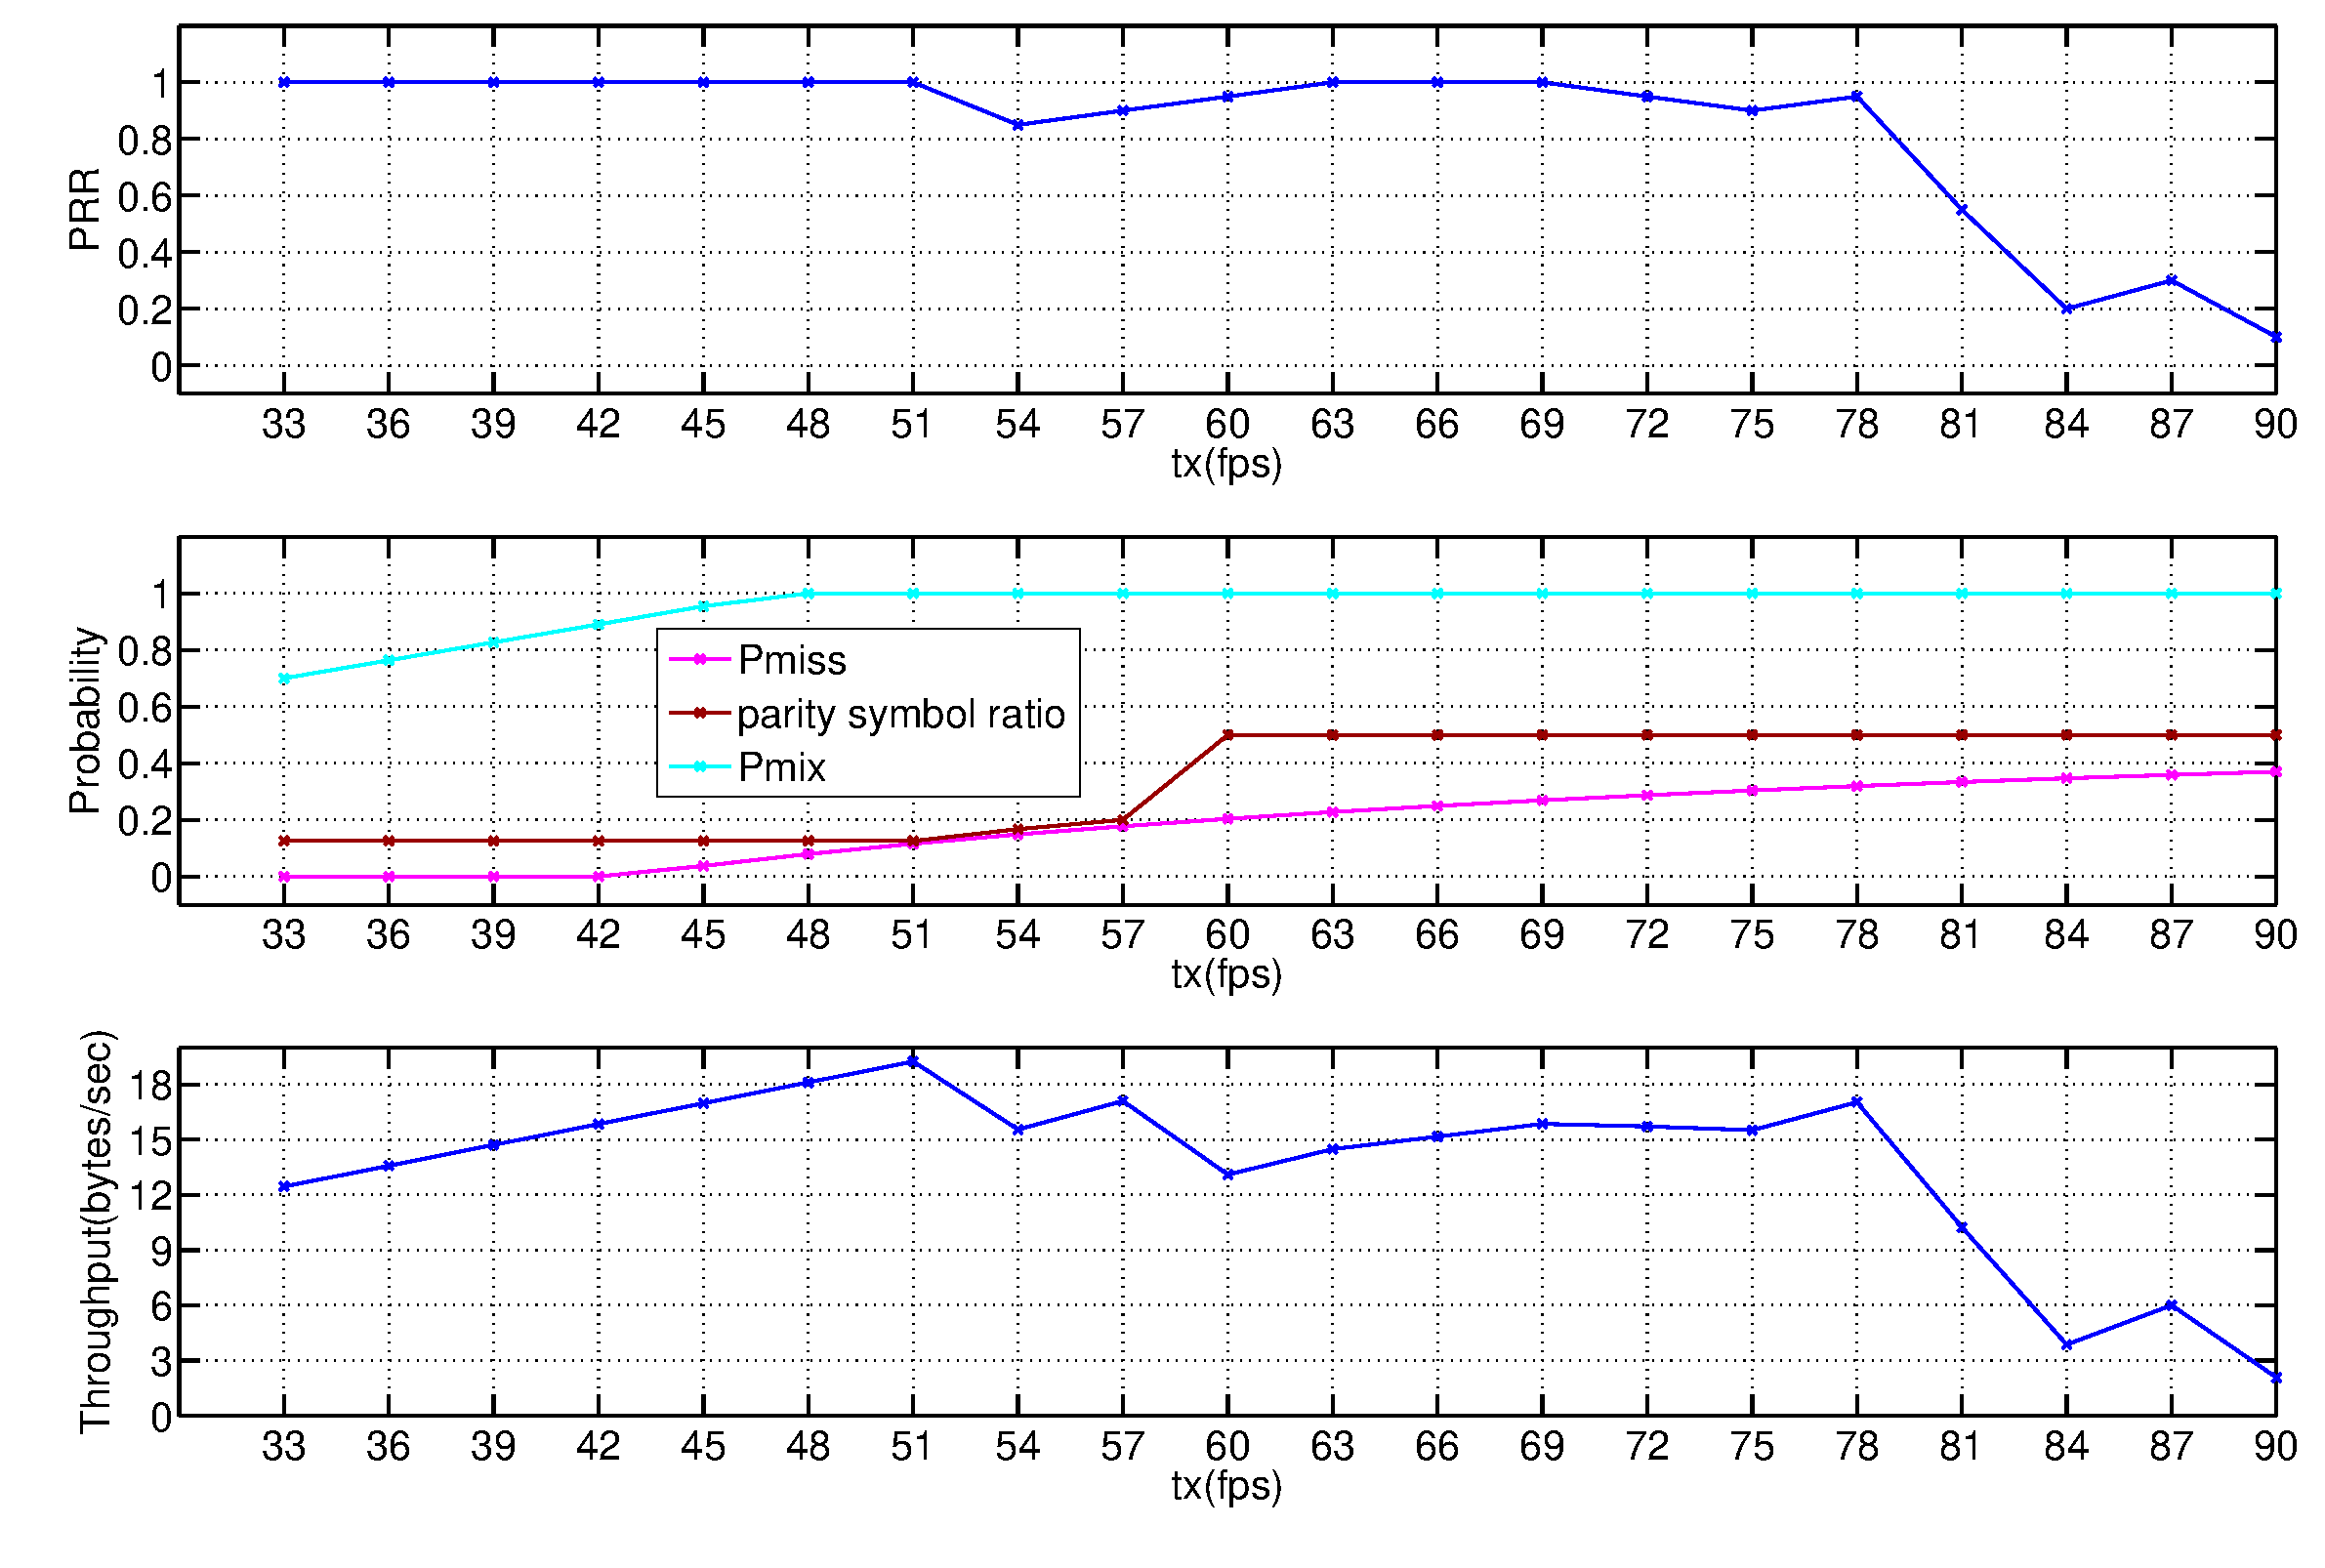
\includegraphics[width=\textwidth]{fig/exp3_iphone5s_new_modify.eps}
	  \caption{}
	  \label{fig:exp3_3}
	\end{subfigure}
	~
	\begin{subfigure}[h]{0.3\textwidth}
	  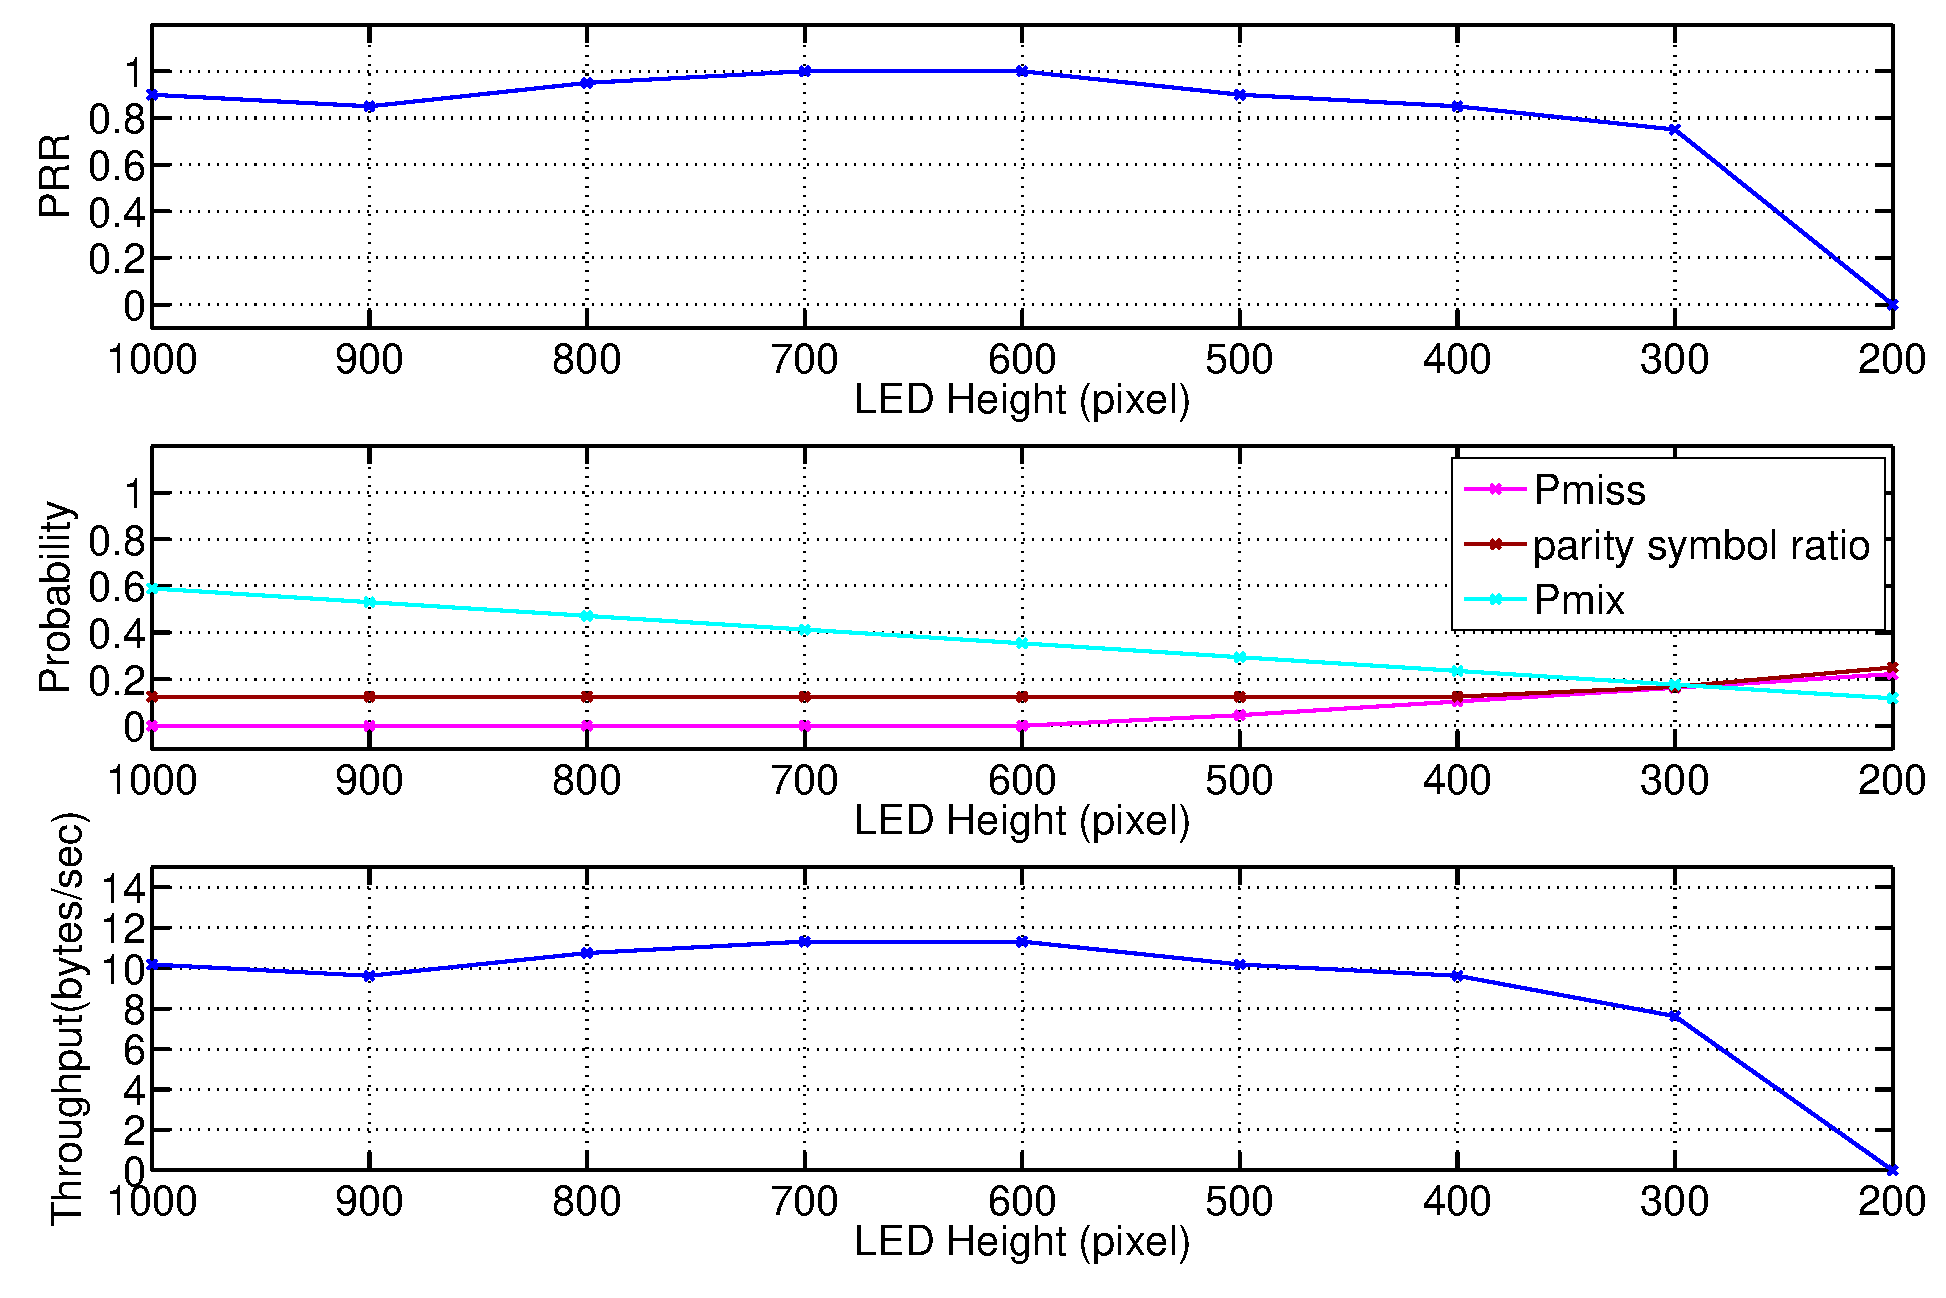
\includegraphics[width=\textwidth]{fig/exp4_iphone5s_new.eps}
	  \caption{}
  	  \label{fig:exp4_2}
	\end{subfigure}
	% ~
	% \begin{subfigure}[h]{0.3\textwidth}
 %  	  \includegraphics[width=\textwidth]{}
 %      \caption{}
 %      \label{}
 %    \end{subfigure}
    \caption{(a) Result of iPhone5s under different transmitting frame rate. (b) Result of iPhone5s under different LED height.}
    \label{}
\end{figure*}

\subsection{Max Throughput under Different Transmitting Frame Rate}
\label{sec:maxthroughput}
In this experiment, we fix the receiving frame rate and gradually increase the transmitting frame rate to determine the maximum achievable throughput, and when we can achieve it. As the transmitting frame rate gets higher, $P_{miss}$ increases, and thus we need to use a higher parity ratio to compensate. However, the transmitted data rate also increases. We would like to investigate at what transmitting frame rate the maximum throughput can be obtained.
In this experiment, we increase the transmitting frame rate from 33 fps to 90 fps. The iPhone5s is at 29.98 fps on average. We only use the third setting in this experiment.

\autoref{fig:exp3_3} shows the result of iPhone5s. We can see $P_{miss}$ grows from 0 to over 0.5, and the parity symbol ratio we select is just above the $P_{miss}$ line. Note that the parity symbol ratio we use is at most 0.5. Because we think the overhead costs too much if a symbol is transmitted over two times. We can see that PRR is more than 90\% until the transmitting frame rate reaches 81 fps. 
Theoretically, the upper limit of the transmitting frame rate is bounded by the case of having two symbols in a received frame, which is given by 
\begin{equation}
%Max\_tx\_fps = \frac{1}{(H - 2*FD\_width) T_r} \qquad \textrm{.}
FPS_{Max,tx}= \frac{1}{(H - 2H_{SD}) T_r} \qquad \textrm{.}
\end{equation}

The max transmitting frame rate for iPhone5s is about 53.39 fps, two symbols in a received frame rarely happens. At that time the parity symbol can be used to recover data. Therefore, we can get even higher transmitting frame rate in practice.

The PRR is above 80\% until reaches the transmitting frame rate of 81 fps. We can see that the iPhone5s can have high PRR when the transmitting frame rate is lower than 81 fps.
We can see the throughput line grows with a trend - at the time the parity symbol ratio increases, the throughput would stay the same or drop a little. The maximum throughput of iPhone5s happens at 51 fps, and the throughput has increased by 1.28 times and reaches 19.25 bytes per second.



\subsection{Different LED Size in the Image}

So far, we have considered the factors of transmitting frame rate, receiving frame rate and the read-out time of the camera. There is one more factor - the image height, which may affect $P_{miss}$ and $P_{mix}$. Thus, in this experiment, we try to change the height of the LED in the received image.
There are two methods to do so, one is use the same setting with the previous experiments (which let the LED light full of the image) and simply crop the image into the height we want. The other is to move the receiver from near to far. We choose the latter method. When we get far away from the LED, although the intensity of light and the detection of the LED boundary may also cause some decoding error, we think the latter method exhibits a setting closer to the real situation. 

We use the height (pixel) of the LED in the received image as our X-axis in \autoref{fig:exp4_2}. The transmitting frame rate is configured to 30 fps. The iPhone5s is at 29.98 fps on average. We only use the third setting in this experiment. As to how far away we can reach, it depends on the sensor size of the camera, the focal length of the lens, and the size of the LED. 
%\autoref{tab:camera_para} lists the parameters of the cameras we use in the experiment. 
If we know all the parameters of the camera and lens, the distance from the LED to the camera is proportional to:

\begin{multline}
	distance (cm) \propto \\
	\frac{focal\_length (mm) * LED\_height (mm) * image\_height (pixels)}{LED\_height (pixels) * sensor\_height (mm)} 
	\qquad \textrm{.}
\end{multline}

We also provide a comparison in ~\autoref{tab:comp_dis}, showing the relationship between the distance and LED height in the received image of Flea3 and iPhone5s. The real LED height we use in the experiment is 4.7 cm. In the table, we can see if the LED object in the image is around 500 pixel, the distance from the object to the Flea3 can be half a meter, while the iPhone5s can only be 15 centimeters. However, if the size of the image area illuminated by the light becomes bigger, (For transmitter-end, we can simply use the lampshade to enlarge the light range. For receiver-end, we can use the reflected light from surrounding areas, such as a wall.) we can further lift the distance limitation. 

% \begin{table}[!htb]
% \centering
% \caption{Camera parameters of Flea3 and iPhone5s.}
%   %large
%   \begin{tabular}{lcc}
%   \hline Parameters & Flea3 & iPhone5s \\
%   \hline 
%   \hline Camera Sensor Format & 1/2.5" & 1/3" \\
%   \hline Image Height(pixel) & 1080 & 1080\\
%   \hline Pixel Size($\mu$m) & 1.55 & 1.5 \\
%   \hline Focal Length(mm) & 16 & 4.21 \\
%   \end{tabular}
%   \label{tab:camera_para} 
% \end{table}

Note that we still have a limitation that the transmitting symbol in the received image need to occupy at least two black-white strips for detecting the signal period. For example, symbol with the largest strip width received from Flea3 is 58 pixel, so the image area need to have at least a height of 232 pixel. It means if the height of LED in the received image is smaller than 232 pixel, then the received symbol cannot be decoded.

\begin{table*}[!t]
\centering
\caption{Distance table of Flea3 and iPhone5s.}
  %\large
  \hspace{-2em}
  \tabcolsep=0.11cm
  \begin{tabular}{lcccccccccc}
  \hline LED height in image (pixel) & 1000 & 900 & 800 & 700 & 600 & 500 & 400 & 300 & 200 & 100 \\
  \hline 
  \hline Flea3 distance (cm) & 48.5 & 53.9 &60.6& 69.3 &80.9& 97.0& 121.3 &161.7 &242.6 &485.2\\
  \hline iPhone5s distance (cm) & 7.75& 8.61& 9.68& 11.07& 12.91& 15.49& 19.36& 25.82& 38.73& 77.46 \\
  \end{tabular}
  \label{tab:comp_dis} 
\end{table*}


\autoref{fig:exp4_2} shows the results of iPhone5s, due to its longer read-out time and shorter time gap between receiving frames, $P_{miss}$ is relatively smaller. Thus, when the LED has a height of around 300 pixel in the image, the transmission can still be received. The PRR is about 75\%.
 
 We can see the iPhone5s can achieve 9.5 $\sim$ 12 bytes per second when the LED height is above 500 pixel. As the LED object in the image becomes small, the throughput decreases significantly; due to both a smaller PRR and a large parity symbol ratio.


\subsection{Time Measurement of Real-time iOS Decoder App}
\label{sec:ios_eval}
%(needed if preview mode is not equal to video mode)
%(Figure: x:tx/rx ratio, y:PRR, color line:mode, for iphone5s app)

We have shown that our system work well for cameras on mobile devices. In this subsection, we want to know whether the decoding process can be executed in real-time with smartphone processors, we also implement an iOS decoding app, running on iPhone5s.

We use the AV Foundation framework, which provides an Objective-C interface for managing and playing audio-visual media in iOS applications. The application uses multiple threads. One thread obtains the frame buffers captured by the camera, and put the image buffers into the queue to be processed. The other thread takes the frame at the front of the queue and decodes it in real time without saving the image. Decoding results for the frame will be shown on the phone screen. \autoref{fig:ios_gui} shows the GUI of the iOS application; one can first touch the screen where the light locates to lock the focus and the exposure time. After pressing start button, the application will start to detect the LED location and decode the message.

% \begin{figure}[!t]
%   \centering
%   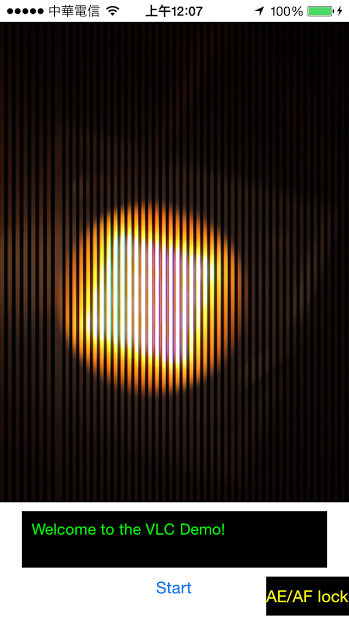
\includegraphics[scale=0.25]{fig/ios_gui3.png}
%   \caption{iOS application GUI}
%   \label{fig:ios_gui}
% \end{figure}

\begin{figure}[!t]
  \centering
  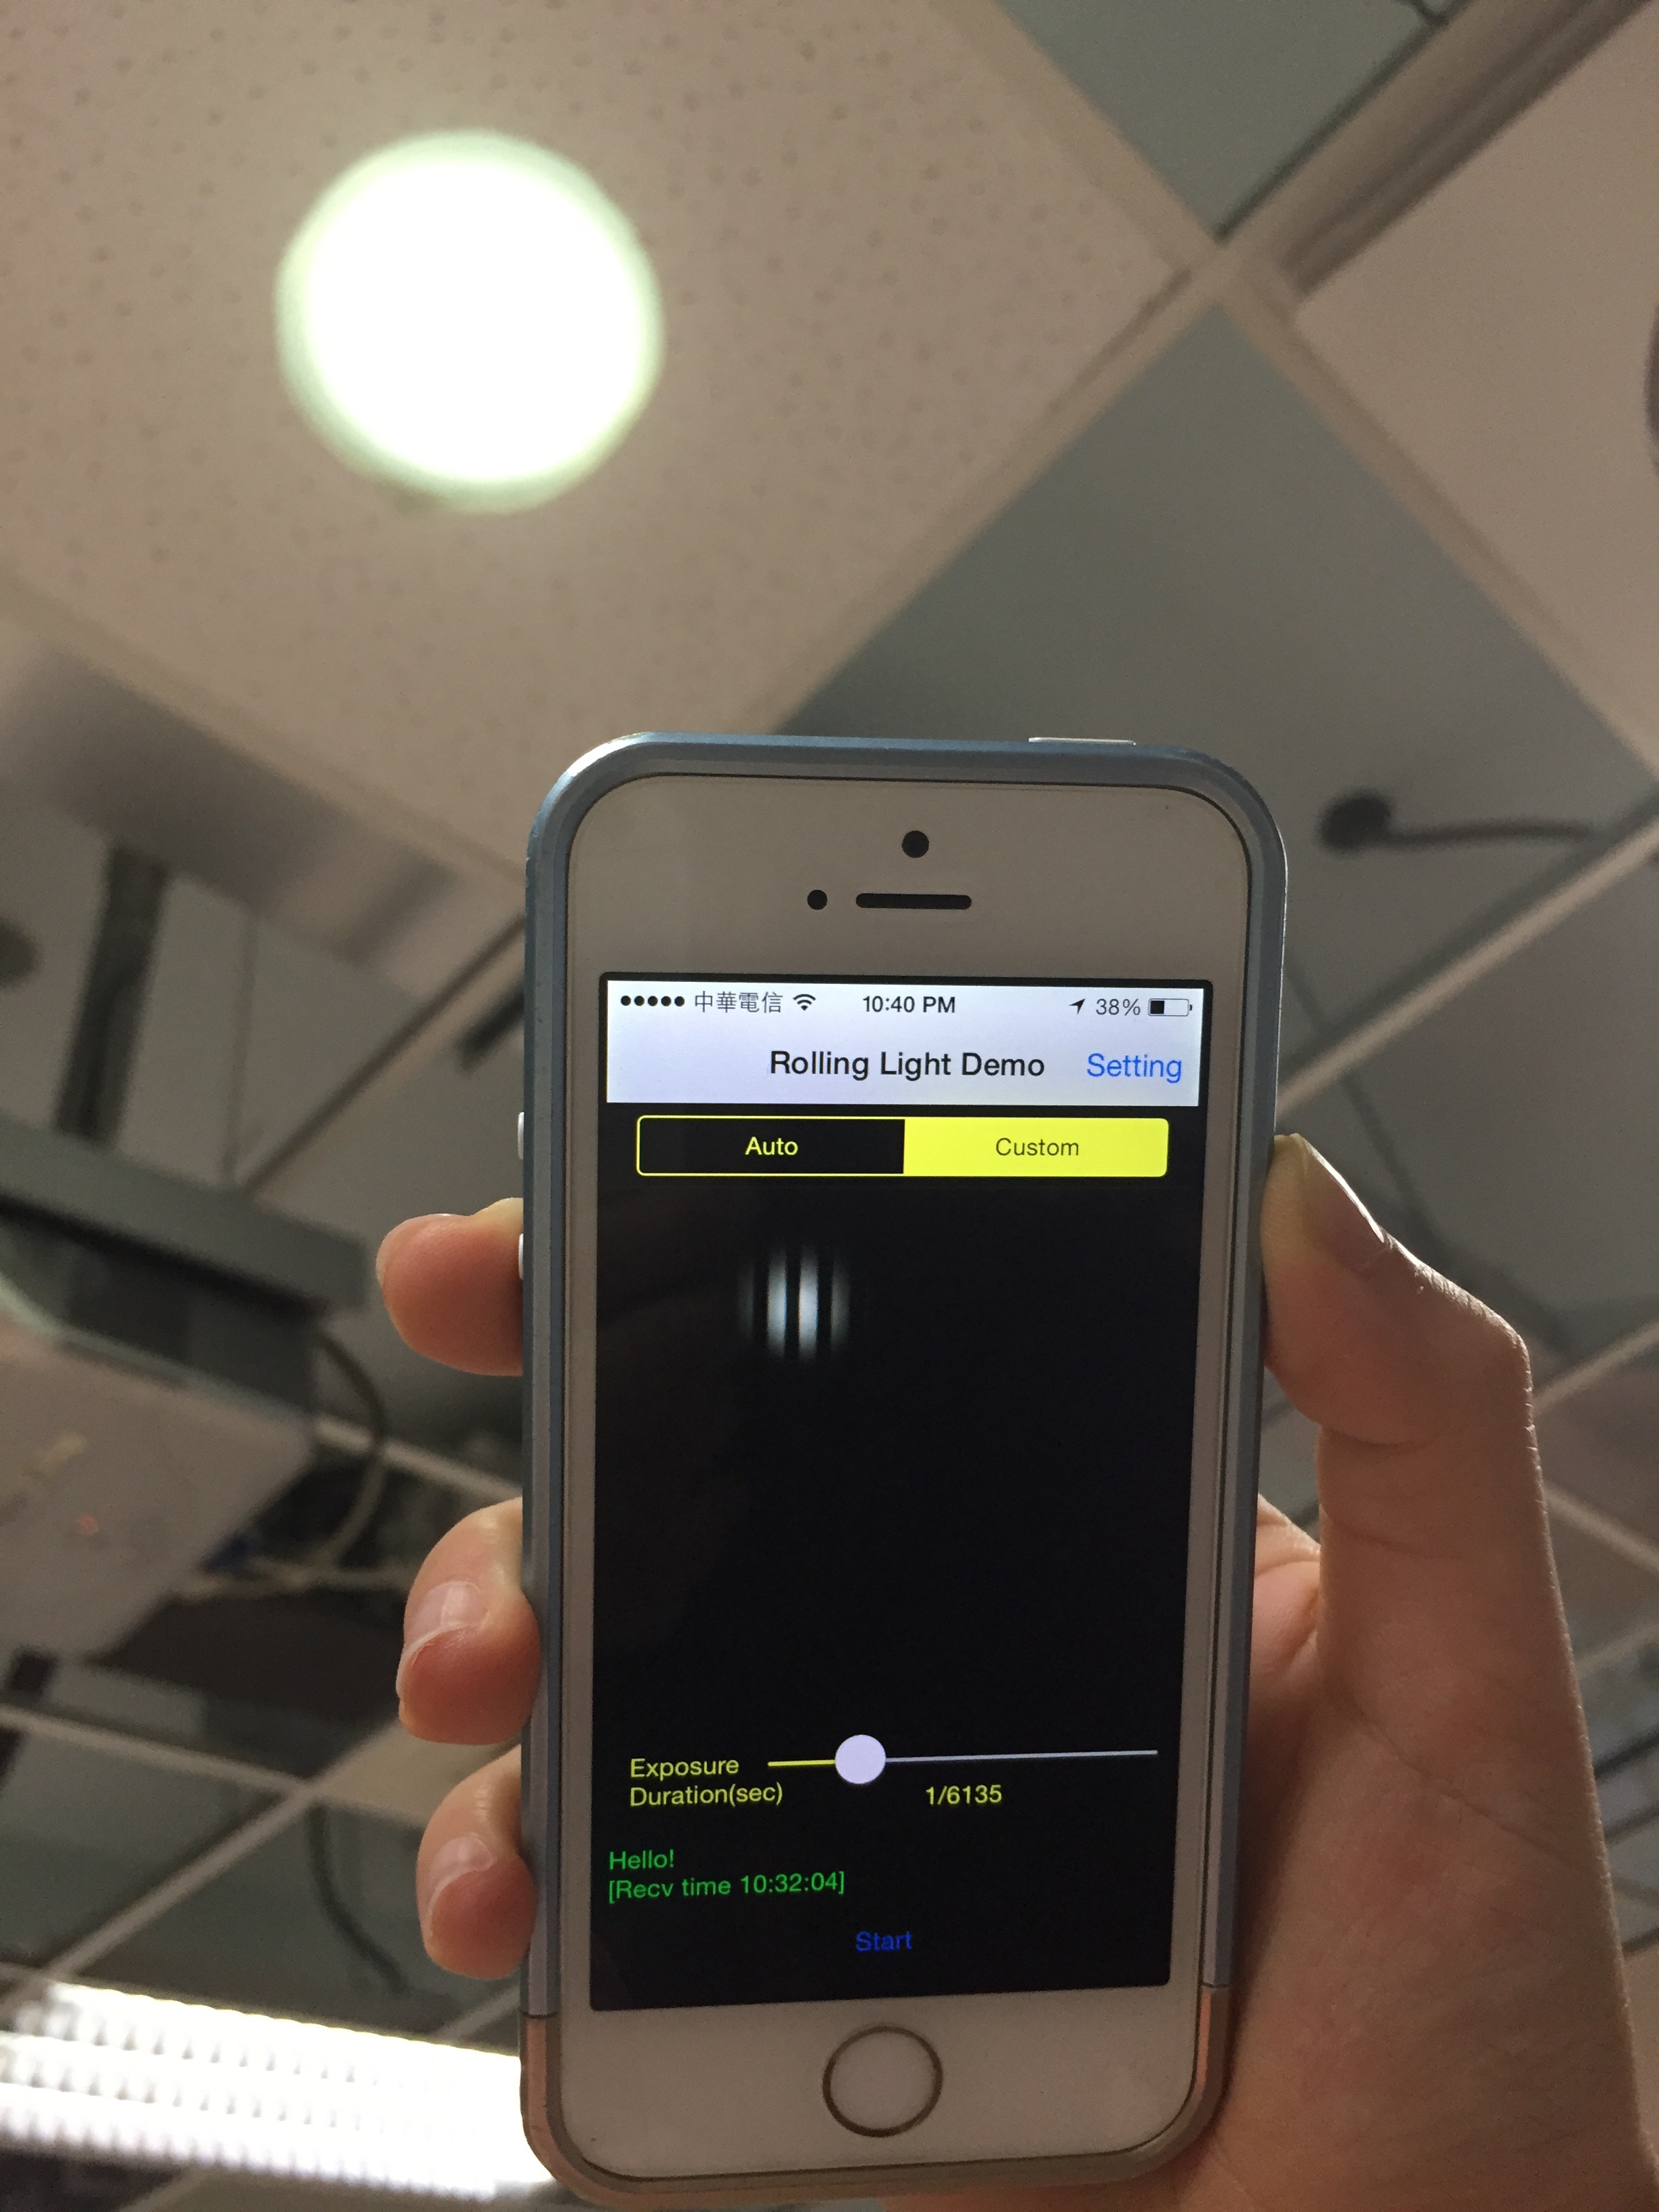
\includegraphics[scale=0.075]{pic/ios_using.JPG}
  \caption{iOS application GUI}
  \label{fig:ios_gui}
\end{figure}

%\subsection{Optimizations for real-time processing}
Since we have set the FrameDuration of the captured video data output (for example, we set the video to 30 fps), we need to make sure that we have enough time to process a frame within one FrameDuration.

To optimize the processing time, we first add the optimization level of Apple LLVM 5.1 compiler as "-Os", generating a faster and smaller executable.

Next, we time individual operations to assess their computational complexity. We found that the majority of the processing time happens when we try to get the frame buffer and convert it to the UIImage, then convert the UIImage to the OpenCV Mat type. This step takes about 0.04 sec, which is greater than a frame duration. To reduce the time, we directly get the pixel base address and put it into Mat. Surprisingly, the time reduces to 0.00003 sec.

Moreover, we found that when we convert RGB to gray scale, it also costs about 0.02 sec. To reduce the time, we change the video output pixel format to YUV color space, and use the luminance(Y) channel as the gray scale value. As a result, we save 0.02 sec.

After a series of optimizing steps, the total processing time of a frame is about 0.007 sec which is less than $1/30$ sec. Since our current implementation already meets the real-time target, we do not explore further optimizations, even though some operations could be sped up more.
 \autoref{tab:ios_time} lists the time taken for each operation.

\begin{table}[!t]
\centering
\caption{Processing time breakdown in ms}
        %\tabcolsep=1cm
        %\large
        \begin{tabular}{lc}
        \hline Operation & time(ms) \\ \hline \hline
        Image Buffer to Mat Conversion & 0.03 \\
        Symbol Delimiter Detection & 3.25 \\
        YIN Period Detection & 3.74 \\
        GUI Text Output & 0.04 \\
        \hline
        Total & 7.06 \\
        \hline
        \end{tabular}
        \label{tab:ios_time}
\end{table}
\section{Conclusion and future work}

\subsection{Conclusion}
In this thesis, we implemented a CamCom system that utilizes a \textbf{single LED} as the transmitter and a common \textbf{rolling shutter CMOS camera} as the receiver. We presented considerations for addressing issues caused by unsynchronized transmitter and receiver, including the introduction of \textbf{symbol delimiter, sequence number, and parity symbol} in the transmission. In each situation, we calculate the probability of symbol loss and mixed frame first, then decide which setting is suitable and adjust the parity symbol ratio by the probability. 

Experimental results confirm that the additional designs would significantly improve the packet reception rate (PRR) from 0.6 to 0.99 when the transmitting and receiving frame rates are close. We also can improve the PRR from 0.0 to 0.8$\sim$1.0 even when the transmitting and receiving frame rates have a large difference or when the the receiving frames have varying inter-frame intervals. A variety of front/ back-facing cameras of smartphones can be used in our system without any modification. One can increase the throughput by 1.2 times by increasing the transmitting frame rate. Data still can be received when the height of LED object in the image is more than 400 pixel. The overall throughput reaches 18 bytes per second. The decoding application proves that series of step can be processed in real-time, with each image frame completely demodulation in merely 7 milliseconds.

\subsection{Future Work}
\textbf{Improve the iOS real-time decoding app.} There are many things can be improved. First is the LED detection. For now, we just threshold the image to binary and find the bright part as the boundary. However, it is not an efficient way and is affected by the surrounding light noise. We want to adopt the characteristics of the strips and use some Digital Image Processing (DIP) techniques to figure out.
On the other hand, to get shorter exposure time, the current method is to move the camera to be very close to the LED light and lock the exposure time. It is not convenient in the real life scenarios since we are not able to get very close to the light. The Landmark paper~\cite{landmark} have proposed the algorithm which find the brightest part in the image then focus/ expose at it, which could be adapted to our system.

\textbf{Increase the data rate.} There are severals ways to increase the data rate, we have tried increasing the transmitting frame rate. We also can increase the number of bits represented by each symbol. We can obtain a higher data rate with more transmitting symbols to carry the bits.

\textbf{Consider more scenarios.} Currently we focus on the static environments. We still need to do more experiments in the moving scenario or dynamic environments to access the feasibility and reliability of our design.
\section{ACKNOWLEDGEMENTS}

This work is supported in part by National Science Council, National Taiwan University, and Intel Corporation under grants NSC-102-2911-I-002-001, NSC-102-2221-E-002-093-MY2, and NTU-103R7501.


%
% The following two commands are all you need in the
% initial runs of your .tex file to
% produce the bibliography for the citations in your paper.
\bibliographystyle{IEEEtran}
\bibliography{rollinglight}  % sigproc.bib is the name of the Bibliography in this case
% You must have a proper ".bib" file
%  and remember to run:
% latex bibtex latex latex
% to resolve all references
%
% ACM needs 'a single self-contained file'!
%
%APPENDICES are optional
%\balancecolumns

%\appendix

\end{document}
